%--------------------------------------------------------------------%
%
% Berkas utama templat LaTeX.
%
% author Petra Barus, Peb Ruswono Aryan, Faris Rizki Ekananda
%
%--------------------------------------------------------------------%
%
% Berkas ini berisi struktur utama dokumen LaTeX yang akan dibuat.
%
%--------------------------------------------------------------------%

\documentclass[bahasa, 12pt, a4paper, onecolumn, oneside, final]{report}

%-------------------------------------------------------------------%
%
% Konfigurasi dokumen LaTeX untuk laporan tesis IF ITB
%
% @author Petra Novandi
%
%-------------------------------------------------------------------%
%
% Berkas asli berasal dari Steven Lolong
%
%-------------------------------------------------------------------%

% Ukuran kertas
\special{papersize=210mm,297mm}

% Setting margin
\usepackage[top=3cm,bottom=3cm,left=4cm,right=3cm]{geometry}

\usepackage{mathptmx}

% Judul bahasa Indonesia
\usepackage[bahasa]{babel}

% Format citation
\usepackage[style=apa,backend=biber]{biblatex}

\usepackage[utf8]{inputenc}
\usepackage{graphicx}
\usepackage{titling}
\usepackage{blindtext}
\usepackage{sectsty}
\usepackage{chngcntr}
\usepackage{etoolbox}
\usepackage[hidelinks]{hyperref}       % Package untuk link di daftar isi. Ubah jadi \usepackage[hidelinks]{hyperref} apabila ingin menghilangkan kotak merah disekitar link
\usepackage{titlesec}       % Package Format judul
\usepackage{titletoc}       % Package Format judul di toc
\usepackage{tocbibind}      % Package untuk masukkan toc, lot, lof ke Daftar Isi
\usepackage{scrwfile}       % Package untuk membuat Daftar Lampiran dari toc
\usepackage{parskip}
\usepackage{afterpage}
\usepackage{relsize}
\usepackage{enumitem}
\usepackage[center]{caption}
\usepackage[none]{hyphenat}  % Package untuk matiin hypenation 
\usepackage{longtable}
\usepackage{url}
\usepackage{placeins}
\usepackage{ragged2e}
\usepackage[table,xcdraw]{xcolor}
\usepackage{array}
\usepackage{lscape}
\usepackage{hhline}
\usepackage{setspace}

%multi-row
\usepackage{multirow}

\graphicspath{{resources/}}   % letak direktori penyimpanan gambar

% Setting daftar lampiran
\newcommand*{\lopname}{DAFTAR LAMPIRAN}
\TOCclone[\lopname]{toc}{atoc}
\addtocontents{atoc}{\protect\value{tocdepth}=-1}
\newcommand\listofappendices{
  \cleardoublepage
  \phantomsection
  \listofatoc
  \addcontentsline{toc}{chapter}{\lopname}
}

\newcommand*\savedtocdepth{}
\AtBeginDocument{%
  \edef\savedtocdepth{\the\value{tocdepth}}%
}

\let\originalappendix\appendix
\renewcommand\appendix{%
  \originalappendix
  \cleardoublepage
  \addtocontents{toc}{\protect\value{tocdepth}=-1}%
  \addtocontents{atoc}{\protect\value{tocdepth}=\savedtocdepth}%

  \titlecontents{chapter}
    [0pt]
    {\bfseries}
    {Lampiran \thecontentslabel.\quad}
    {}
    {\dotfill\contentspage}

  \titleformat{\chapter}[block]
    {\bfseries}
    {\chaptertitlename\ \thechapter.\quad}{0pt}
    {\bfseries}
}

% Hilangkan titik pada toc
\makeatletter
\renewcommand{\@dotsep}{1} 
\makeatother

% Setel title pada chapter-chapter di toc, lof, lot
\titlecontents{chapter}
  [0pt]
  {\bfseries}
  {\MakeUppercase{Bab} \thecontentslabel\quad\uppercase}
  {}
  {\dotfill\contentspage}
\titlecontents{figure}
  [0pt]
  {}
  {Gambar \thecontentslabel.\quad}
  {}
  {\dotfill\contentspage}
\titlecontents{table}
  [0pt]
  {}
  {Tabel \thecontentslabel.\quad}
  {}
  {\dotfill\contentspage}

% Masukin Daftar Pustaka ke toc
\let\originalprintbibliography\printbibliography
\renewcommand\printbibliography{%
  \phantomsection
  \cleardoublepage
  \originalprintbibliography
  \addcontentsline{toc}{chapter}{\bibname}
}

% Line satu setengah spasi
\renewcommand{\baselinestretch}{1.5}

% Setting judul
\chapterfont{\centering \Large}
\titleformat{\chapter}[display]
  {\Large\centering\bfseries}
  {\chaptertitlename\ \thechapter}{0pt}
    {\Large\bfseries\uppercase}

% Setting nomor pada subbsubsubbab
\setcounter{secnumdepth}{3}

\makeatletter

\makeatother

% Counter untuk figure dan table.
\counterwithin{figure}{chapter}
\counterwithin{table}{chapter}

% Define blank page
\newcommand*{\blankpage}{\afterpage{\null\newpage}}

% Define list with less spacing
\setlist{noitemsep}

\makeatletter

\makeatother

\addbibresource{references.bib}

\begin{document}

\sloppy

%Basic configuration
\title{PERANCANGAN DESAIN INTERAKSI APLIKASI PENCEGAH DISTRAKSI \textit{DIGITAL WELLBEING} DENGAN PENDEKATAN \textit{USER-CENTERED DESIGN}}
\date{}
\author{
    GREGORIUS JOVAN KRESNADI \\
    NIM : 13518135
}

\pagenumbering{roman}
\setcounter{page}{1}

\clearpage
\pagestyle{empty}

\begin{center}
    \smallskip
    
    \Large \bfseries \MakeUppercase{\thetitle}
    \vfill
    
    \Large Laporan Tugas Akhir
    \vfill
    
    \large Disusun sebagai syarat kelulusan tingkat sarjana
    \vfill
    
    \large Oleh
    
    \Large \theauthor
    
    \vfill
    \begin{figure}[h]
        \centering
        
\includegraphics[width=0.15\textwidth]{cover-ganesha.jpg}
    \end{figure}
    \vfill
    
    \large
    \uppercase{
        Program Studi Teknik Informatika \\
        Sekolah Teknik Elektro \& Informatika \\
        Institut Teknologi Bandung
    }
    
    Agustus 2022
    
\end{center}

\clearpage

\clearpage
\pagestyle{empty}

\begin{center}
    \smallskip

    \Large \bfseries \MakeUppercase{\thetitle}
    \vfill

    \Large Laporan Tugas Akhir
    \vfill

    \large Oleh

    \Large \theauthor

    \large Program Studi Teknik Informatika \\

    \normalsize \normalfont
    Sekolah Teknik Elektro dan Informatika \\
    Institut Teknologi Bandung \\

    \vfill
    \normalsize \normalfont
    Telah disetujui dan disahkan sebagai draft Laporan Tugas Akhir \\
    di Bandung, 02 September 2022 \\
    Mengetahui,

    \vspace{0.5cm}
    Pembimbing,

    \vfill
    \underline{Adi Mulyanto, S.T, M.T.} \\
    NIP. 19631126 198803 1 002

\end{center}
\clearpage
 % 1 PEMBIMBING PAKAI INI
% \clearpage
\pagestyle{empty}

\begin{center}
    \smallskip

    \Large \bfseries \MakeUppercase{\thetitle}
    \vfill

    \Large Laporan Tugas Akhir
    \vfill

    \large Oleh

    \Large \theauthor

    \large Program Studi Teknik Informatika \\

    \normalsize \normalfont
    Sekolah Teknik Elektro dan Informatika \\
    Institut Teknologi Bandung

    \vfill
    \normalsize \normalfont
    Bandung, 15 November 2021 \\
    Mengetahui,

    \vspace{0.5cm}
    \setlength{\tabcolsep}{12pt}
    \begin{tabular}{c@{\hskip 0.5in}c}
        Pembimbing I,                           & Pembimbing II,                           \\
                                                &                                          \\
                                                &                                          \\
                                                &                                          \\
                                                &                                          \\
        \underline{Nama dan Gelar Pembimbing I} & \underline{Nama dan Gelar Pembimbing II} \\
        NIP. 123456789                          & NIP. 123456789                           \\
    \end{tabular}

\end{center}
\clearpage
 % 2 PEMBIMBING PAKAI INI
\chapter*{Lembar Pernyataan}

Dengan ini saya menyatakan bahwa:

\begin{enumerate}

    \item Pengerjaan dan penulisan Laporan Tugas Akhir ini dilakukan tanpa menggunakan bantuan yang tidak dibenarkan.
    \item Segala bentuk kutipan dan acuan terhadap tulisan orang lain yang digunakan di dalam penyusunan laporan tugas akhir ini telah dituliskan dengan baik dan benar.
    \item Laporan Tugas Akhir ini belum pernah diajukan pada program pendidikan di perguruan tinggi mana pun.

\end{enumerate}

Jika terbukti melanggar hal-hal di atas, saya bersedia dikenakan sanksi sesuai dengan Peraturan Akademik dan Kemahasiswaan Institut Teknologi Bandung bagian Penegakan Norma Akademik dan Kemahasiswaan khususnya Pasal 2.1 dan Pasal 2.2.
\vspace{15mm}

Bandung, 02 September 2022 
\vspace{2.5cm}
\\
\underline{Gregorius Jovan Kresnadi} \\
NIM. 13518135
\vfill

\pagestyle{plain}

% \clearpage
\chapter*{ABSTRAK}
\addcontentsline{toc}{chapter}{ABSTRAK}

\begin{center}
  \textbf{\MakeUppercase{\thetitle}} \\[1em]
  
  Oleh: \\
  \MakeUppercase{\theauthor} \\
\end{center}

\begin{singlespace}
  % $ latar belakang
  Penggunaan \textit{smartphone} yang semakin tinggi mempengaruhi kesejahteraan digital dari penggunanya secara negatif.
  Penggunaan \textit{smartphone} yang terlalu tinggi dapat membuat pengguna memiliki ketergantungan terhadap \textit{smartphone} hingga mencapai tingkat adiksi.
  Kasus ini memunculkan urgensi atas penelitian di bidang \textit{Human Computer Interaction} tentang kesengajaan untuk tidak menggunakan teknologi.
  Penelitian ini memunculkan konsep \textit{Digital Wellbeing} yang diadopsi Google untuk mengembangkan sebuah aplikasi berkonsep tersebut.
  Namun ditemukan bahwa aplikasi tersebut memiliki beberapa masalah yang tercerminkan pada banyaknya keluhan pada ulasan aplikasi tentang keterbatasan utilitas.
  
  % $ proses penelitian
  Oleh karena itu, diperlukan sebuah desain interaksi aplikasi yang dapat mengatasi masalah-masalah dari aplikasi Digital Wellbeing.
  Proses perancangan menggunakan metodologi \textit{User-Centered Design}.
  Pengumpulan data diawali dengan menganalisis ulasan dari aplikasi Digital Wellbeing, kemudian dilengkapi dengan wawancara kepada pengguna aplikasi.
  Hasil tugas akhir berupa prototipe \textit{high-fidelity} aplikasi untuk tampilan perangkat \textit{mobile} Android.
  Desain interaksi memprioritaskan \textit{usability goals utility} dan \textit{learnability}, serta mengarahkan kepada \textit{user experience goals helpful} dan \textit{motivating}.
  
  % $ hasil penelitian
  Pengujian dilakukan dengan \textit{usability testing} kepada target pengguna yang sesuai dengan persona yang ditentukan, menggunakan metrik pengukuran SUS, SEQ, dan IMI untuk subskala \textit{Value/Usefulness}, \textit{Interest/Enjoyment}, dan \textit{Pressure/Tension} untuk mengukur ketercapaian \textit{goals}.
  Hasil pengujian menunjukkan bahwa prototipe berhasil menyelesaikan masalah-masalah yang ditemukan, serta mencapai \textit{goals} yang diharapkan.
  Dari pengujian disimpulkan bahwa fitur Search bar, App Group, dan Daftar Jadwal Aktivasi dari prototipe berperan besar dalam meningkatkan utilitas aplikasi, serta fitur Daily Goal menjadi fitur unggulan dalam meningkatkan motivasi pengguna dalam memperbaiki kebiasaan digitalnya.

\noindent \textbf{Kata kunci:} \textit{Digital Wellbeing}, desain interaksi, \textit{user-centered design}, prototipe, \textit{widget}
\end{singlespace}
% \clearpage
\chapter*{Abstract}
\addcontentsline{toc}{chapter}{Abstract}

%put your abstract here
\blindtext

\clearpage
% \chapter*{\MakeUppercase{Kata Pengantar}}
\addcontentsline{toc}{chapter}{KATA PENGANTAR}

Puji syukur penulis ucapkan kepada Tuhan Yang Maha Esa atas berkat dan rahmat-Nya, sehingga penulis dapat menyelesaikan laporan penelitian tugas akhir ini yang berjudul "{\thetitle}". Keberhasilan penulis dalam menyelesaikan laporan ini tidak terlepas dari dukungan dan bantuan dari berbagai pihak. Untuk itu, penulis mengucapkan terima kasih kepada:

\begin{enumerate}
  \item Bapak Adi Mulyanto, S.T, M.T., selaku dosen pembimbing tugas akhir atas bimbingan dan masukan yang diberikan selama masa pengerjaan tugas akhir.
   
  % \item ... selaku dosen penguji tugas akhir yang telah memberikan saran, kritik, dan rekomendasi 
   
  \item Bapak Dicky Prima Satya, S.T., M.T., Bapak Adi Mulyanto, S.T., M.T., Ibu Latifa Dwiyanti, S.T., M.T., dan Bapak Nugraha Priya Utama, S.T., M.A., Ph.D., selaku koordinator tim tugas akhir yang memberikan arahan dalam pengerjaan tugas akhir ini,

  \item Ibu Dessi Puji Lestari, S.T., M.Eng., Ph.D., selaku Ketua Program Studi Teknik Informatika Institut Teknologi Bandung,
   
  \item Bapak Dr. Techn. Muhammad Zuhri Catur Candra, S.T, M.T. dan Ibu Ginar Santika Niwanputri, S.T, M.Sc., selaku dosen wali yang telah membimbing penulis selama berkuliah tiga tahun di Teknik Informatika,
  
  \item Bapak Yudistira Dwi Wardhana Asnar, S.T., Ph.D. yang telah memberikan ide dan inspirasi mengenai topik dari tugas akhir yang dikerjakan, 
  
  \item Para karyawan dan staff dari TU STEI yang telah membantu kebutuhan administrasi dalam menyelesaikan laporan Tugas Akhir,
  
  \item Orang tua, kakak, dan keluarga penulis yang senantiasa memberikan dukungan dan semangat selama menjalani perkuliahan di Teknik Informatika,

  \item Hollyana Puteri Haryono, selaku rekan terdekat penulis yang bersedia menemani serta memberikan semangat dan inspirasi dalam mengerjakan tugas akhir ini,
  
  % \item Teman-teman dari grup "Bunker": Naufal "Bapak" Prima, Michel "Peng" Fang, Junho Choi "Oppa" Hedyatmo, Jonathan "Jojo" Yudi, Matthew "Mek" Kevin, Kamal "Mastree" Shafi, Garry "Geri" Kuwanto, Morgen "Koh" Sudyanto, Muhammad "Euy" Hasan, Fabian "God" Zhafransyah, Reyvan "Berayfun" Rizky, Mario "Margun" Gunawan, Vincent "Lie" Lienardo, Faris "KissShot" Kautsar, Farras Hibban, Nafkhan "Camcam" Alzamzami, Fauzan "Kakek" Rafi, dan Naufal Dean yang telah memberi dukungan, bantuan, dan kata-kata pedas kepada penulis serta memberi hiburan  dengan menjadi teman-teman terbaik dalam masa perkuliahan.
  
  \item Teman-teman dari grup "Bunker": Naufal Prima, Michel Fang, Junho Choi, Jonathan Yudi, Matthew Kevin, Kamal Shafi, Garry Kuwanto, Morgen Sudyanto, Muhammad Hasan, Fabian Zhafransyah, Reyvan Rizky, Mario Gunawan, Vincentius Lienardo, Faris Kautsar, Farras Hibban, Camcam, Fauzan Rafi, dan Naufal Dean, yang telah memberi dukungan, bantuan, dan kata-kata pedas kepada penulis untuk mendorong penulis dalam mengerjakan tugas akhir, serta memberi hiburan dengan menjadi teman-teman terbaik dalam masa perkuliahan,
  
  \item Teman sebimbingan yang bersedia untuk saling menyemangati dan memberikan pendapat, kritik, saran terkait tugas akhir penulis,
  
  \item Teman-teman dari grup "Latex TA pipel", terutama Faris Rizki Ekananda, yang telah membantu penulis dalam mengatur format dokumen laporan tugas akhir,
  
  \item Gitta, Gian, dan teman-teman dari FNFBandung yang senantiasa menjadi penghibur dan penjaga kesehatan fisik maupun mental penulis selama pengerjaan tugas akhir,
  
  \item Para narasumber yang bersedia untuk membantu penulis sebagai partisipan pengumpulan data dan pengujian,

  \item Teman-teman mahasiswa Program Studi Teknik Informatika ITB 2018 yang senantiasa memberikan dukungan dan semangat dalam pengerjaan Tugas akhir,
   
  \item Pihak-pihak lain yang tidak dapat disebutkan satu per satu yang turut serta membantu penulis untuk menyelesaikan Tugas Akhir.
   
\end{enumerate}

Akhir kata, semoga penelitian tugas akhir ini dapat bermanfaat bagi semua pihak yang membutuhkannya

\vspace{15mm}

\begin{flushright}
  Bandung, 02 September 2022 \\
  \vspace{2.5cm}
  Penulis
\end{flushright}
\vfill


% Gunakan bagian ini untuk memberikan ucapan terima kasih kepada semua pihak yang secara langsung atau tidak langsung membantu penyelesaian tugas akhir, termasuk pemberi beasiswa jika ada. Utamakan untuk memberikan ucapan terima kasih kepada tim pembimbing tugas akhir dan staf pengajar atau pihak program studi, bahkan sebelum mengucapkan terima kasih kepada keluarga. Ucapan terima kasih sebaiknya bukan hanya menyebutkan nama orang saja, tetapi juga memberikan penjelasan bagaimana bentuk bantuan/dukungan yang diberikan. Gunakan bahasa yang baik dan sopan serta memberikan kesan yang enak untuk dibaca. Sebagai contoh: “Tidak lupa saya ucapkan terima kasih kepada teman dekat saya, Tito, yang sejak satu tahun terakhir ini selalu memberikan semangat dan mengingatkan saya apabila lengah dalam mengerjakan Tugas Akhir ini. Tito juga banyak membantu mengoreksi format dan layout tulisan. Apresiasi saya sampaikan kepada pemberi beasiswa, Yayasan Beasiswa, yang telah memberikan bantuan dana kuliah dan biaya hidup selama dua tahun. Bantuan dana tersebut sangat membantu saya untuk dapat lebih fokus dalam menyelesaikan pendidikan saya. ....”. Ucapan permintaan maaf karena kekurangsempurnaan hasil Tugas Akhir tidak perlu ditulis.


\titleformat*{\section}{\centering\bfseries\Large\MakeUpperCase}
\titlespacing*{\chapter}{0pt}{0pt}{1pc}

% Setting judul toc, lot, lof, bib
\renewcommand{\contentsname}{DAFTAR ISI}
\renewcommand{\listfigurename}{DAFTAR GAMBAR}
\renewcommand{\listtablename}{DAFTAR TABEL}
\renewcommand{\bibname}{DAFTAR PUSTAKA}

\tableofcontents
\listofappendices
\listoffigures
\listoftables

\newpage

\titleformat*{\section}{\bfseries\large}
\pagenumbering{arabic}

%----------------------------------------------------------------%
% Konfigurasi Bab
%----------------------------------------------------------------%
\setcounter{page}{1}
\renewcommand{\chaptername}{BAB}
\renewcommand{\thechapter}{\Roman{chapter}}
%----------------------------------------------------------------%

%----------------------------------------------------------------%
% Dafter Bab
% Untuk menambahkan daftar bab, buat berkas bab misalnya `chapter-6` di direktori `chapters`, dan masukkan ke sini.
%----------------------------------------------------------------%
% \pagenumbering{}
\chapter{Pendahuluan}

Bab Pendahuluan secara umum menceritakan landasan kerja dan arah kerja penulis tugas akhir, yang berfungsi untuk mengantar pembaca dalam memahami dan menganalisis laporan tugas akhir secara keseluruhan. Bab ini terdiri dari latar belakang, rumusan masalah, tujuan, batasan masalah, metodologi, dan jadwal pelaksanaan tugas akhir.

\section{Latar Belakang}
\label{sec:latarbelakang}

Teknologi dan internet adalah kebutuhan yang penting dalam kehidupan manusia di abad ke-21 ini. Salah satu bentuk teknologi modern paling berguna yang mudah diakses manusia adalah \emph{smartphone}, di mana akses internet sudah termasuk ke dalamnya. Berdasarkan penelitian yang dikumpulkan oleh \textcite{turner2022howmanysmartphones} pada bankmycell.com, pada tahun 2021 terdapat 6.37 miliar pengguna \emph{smartphone} di dunia atau sekitar 80.68\% dari populasi dunia, di antaranya 160.23 juta adalah penduduk Indonesia.

Banyak pekerjaan manusia yang dapat dilakukan dengan menggunakan berbagai jenis aplikasi yang dapat ditemukan dalam sebuah \emph{smartphone}. Menurut penelitian yang dilakukan oleh BusinessofApps, jumlah aplikasi pada iOS App Store ketika pertama kali diluncurkan pada tahun 2008 adalah 500, pada bulan November tahun 2021 angka tersebut melonjak menjadi 1.85 juta aplikasi. Pengguna Android memiliki lebih banyak pilihan dengan total 2.56 juta aplikasi di Google Play Store. Dengan banyaknya aplikasi tersebut, pada tahun 2020 pengguna \emph{smartphone} telah mengunduh aplikasi sebanyak 142.9 miliar kali, di antaranya 56.1 miliar unduhan adalah untuk aplikasi permainan \emph{mobile}.

Teknologi informasi yang semakin berkembang dapat meningkatkan kesejahteraaan digital, atau digital wellbeing, dari pengguna teknologi tersebut, beberapa caranya adalah meningkatkan koneksi sosial, mendukung kesehatan mental, dan mendukung kebiasaan sehat dengan fleksibilitas dalam praktik kerja. Namun teknologi informasi juga dapat menimbulkan akibat buruk yang memunculkan pola penggunaan teknologi yang tidak sehat. Beberapa contoh dampak buruk yang dimunculkan adalah mudahnya seseorang untuk kehilangan fokus, perasaan \emph{fear of missing out} (FoMO), serta kecanduan digital. Sifat-sifat buruk tersebut dapat lebih sering muncul ketika waktu yang dihabiskan pada dunia maya tidak diimbangi dengan waktu di dunia nyata. \parencite{ALMOURAD2021101778}

Pengaruh buruk seperti yang telah disebutkan di atas serta perilaku adiksi pada \textit{smartphone} telah memunculkan perhatian bagi peneliti di bidang \textit{Human Computer Interaction} (HCI) untuk melakukan studi terhadap kesengajaan untuk tidak menggunakan teknologi. Pada saat ini, terdapat banyak perangkat lunak pada \textit{smartphone} yang bertujuan untuk mengubah perilaku penggunanya, salah satunya dibuat oleh Google. \parencite{Roffarello2019} Untuk membantu penggunanya, Google memiliki aplikasi Digital Wellbeing agar pengguna dapat memanfaatkan teknologi untuk meningkatkan kualitas kehidupannya melainkan menjadi distraksi. Pada websitenya tentang Digital Wellbeing, \textcite{google2019digitalwellbeing} mengatakan: "We’re committed to giving everyone the tools they need to develop their own sense of digital wellbeing. So that life, not the technology in it, stays front and center." 


% Salah satu fitur yang terdapat pada aplikasi Digital Wellbeing adalah Focus Mode, sebuah fitur yang dapat membantu mengurangi distraksi dari \emph{smartphone} berbasis Android dengan cara memblokir sementara aplikasi yang dinilai sebagai distraksi. Focus Mode juga akan mendiamkan notifikasi yang masuk hingga waktu yang ditentukan. Waktu yang diterapkan untuk Focus Mode dapat diatur jadwalnya oleh pengguna. \parencite{android2019digitalwellbeing} Selama Focus Mode aktif, akan terdapat sebuah menu pada bagian notifikasi \emph{smartphone} dengan 2 buah fitur. Fitur "Take a break" yang berbentuk tombol ini dapat memberikan pengguna kembali akses untuk aplikasi yang diblok dengan pilihan waktu 5 menit, 15 menit, atau 30 menit. Tombol ini dapat digunakan jika pengguna ingin beristirahat dan menggunakan aplikasi yang diblok. Fitur "Turn off for now" yang juga berbentuk tombol dapat digunakan untuk memberhentikan Focus Mode hanya untuk hari tersebut. Tombol ini dapat digunakan jika pengguna merasa tugas yang perlu difokuskannya sudah selesai dan ingin menggunakan aplikasi yang diblok untuk sisa harinya. Masalah yang ditemukan dari Focus Mode terletak pada kedua fitur ini. Walau memerlukan interaksi lebih untuk "beristirahat", terdapat kemungkinan bagi pengguna untuk terus menerus mengakses aplikasi, dengan mengambil istirahat setiap beberapa menit sekali. Selain itu, fitur "Turn off for now" dapat disalahgunakan untuk menghindari Focus Mode secara keseluruhan.

\section{Rumusan Masalah}

Penggunaan tinggi \textit{smartphone} dapat mempengaruhi kesejahteraan digital dari penggunanya dalam cara yang negatif. Salah satu bentuk dari hubungan yang tidak baik antara \textit{smartphone} dan penggunanya adalah tingginya tingkat ketergantungan terhadap \textit{smartphone} hingga dapat mencapai tingkat adiksi. Penurunan kualitas hubungan tersebut dapat disebabkan oleh gangguan dari aplikasi pada \textit{smartphone} atau keinginan pengguna sendiri untuk menggunakannya. Dalam upaya memperbaiki hubungan tersebut, Google merilis aplikasi Digital Wellbeing yang bertugas untuk membantu pengguna \textit{smartphone} berbasis Android untuk mengatur kesehatan penggunaannya. Namun, dengan banyaknya aplikasi dengan tujuan serupa di \textit{marketplace} Google Play Store, dapat dilihat bahwa terdapat beberapa batasan pada aplikasi Digital Wellbeing. Maka dari itu, dapat disimpulkan rumusan masalah yang akan didalami dalam Tugas Akhir ini adalah sebagai berikut

\begin{enumerate}
  \item Bagaimana rancangan desain interaksi yang tepat untuk menyelesaikan masalah yang terdapat pada aplikasi pencegah distraksi Digital Wellbeing?
  \item Bagaimana prototipe aplikasi pencegah distraksi Digital Wellbeing dengan desain interaksi menggunakan pendekatan \emph{user-centered design}?
\end{enumerate}

\section{Tujuan}

Berdasarkan latar belakang dan rumusan masalah di atas, tujuan dari Tugas Akhir ini adalah untuk membuat sebuah prototipe aplikasi pencegah distraksi. Prototipe aplikasi tersebut memiliki desain interaksi yang dapat menyelesaikan masalah-masalah desain interaksi yang ditemukan pada alat Digital Wellbeing milik Google.


\section{Batasan Masalah}

Batasan masalah untuk implementasi solusi Tugas Akhir ini adalah sebagai berikut
\begin{enumerate}
  \item Hasil akhir dari studi adalah solusi dalam bentuk prototipe aplikasi untuk \textit{smartphone} berbasis Android dengan versi OS lebih besar sama dengan versi Android 9.0.
  \item Responden penelitian adalah masyarakat Indonesia, dengan rentang umur 18 hingga 30 tahun.
  \item Pengujian akan dilakukan dengan membandingkan penggunaan \textit{smartphone} yang disertai bantuan aplikasi Digital Wellbeing dengan prototipe aplikasi solusi.
\end{enumerate}

\section{Metodologi}
\label{sec:metodologi}

Metodologi dalam perancangan solusi Tugas Akhir menggunakan pendekatan \textit{user-centered design} (UCD) yang mengikuti standar alur kerja dari ISO (\textit{International Organization for Standardization}) 9241-210:2010. Berikut adalah penjelasan dari setiap tahap UCD


\begin{figure}[h]
  \centering
  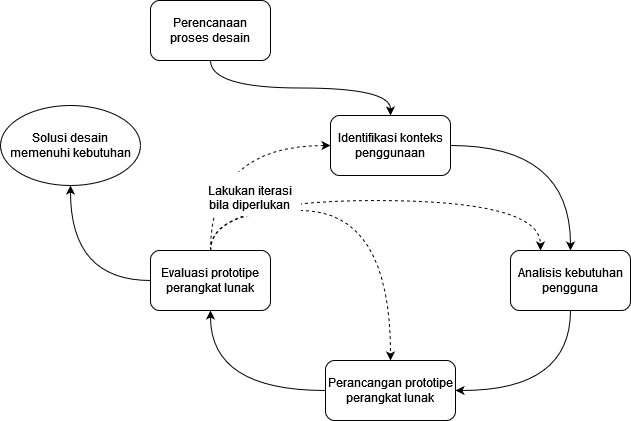
\includegraphics[width=0.9\textwidth]{chapter-1-method.png}
  \caption{Diagram alur pengerjaan \textit{User-Centered Design} (ISO 9241-210, 2010)}
  \label{fig:diagram_iso1}
\end{figure}

\begin{enumerate}
  \item Perencanaan proses desain
  \subitem Proses UCD diawali dengan tahap persiapan, yaitu proses perancangan terhadap lingkup aplikasi yang dibuat serta perencanaan untuk pengambilan data. Lingkup dari aplikasi termasuk jenis antarmuka dan \textit{platform} yang dipilih untuk implementasi, lingkup fungsionalitas aplikasi, serta target pengguna aplikasi. Sedangkan perencanaan pengambilan data dilakukan dengan cara survei dan wawancara.

  \item Identifikasi konteks penggunaan
  \subitem Pada tahap ini dilakukan pengumpulan data pengguna melalui survei dan wawancara sesuai dengan kebutuhan. Data yang didapatkan akan dianalisis untuk mengungkapkan permasalahan, kebutuhan, dan tujuan pengguna. Berdasarkan data riset tersebut akan dibentuk persona serta skenario penggunaan aplikasi, yang kemudian akan dianalisis untuk mendapatkan kebutuhan perangkat lunak.
   
  \item Analisis kebutuhan perangkat lunak
  \subitem Tahap ini terdiri dari analisis fitur perangkat lunak, analisis \textit{user experience goals}, dan analisis \textit{usability goals}. Fitur-fitur yang terkumpul akan menjadi bahan implementasi pada tahap selanjutnya.
  
  \item Perancangan prototipe perangkat lunak
  \subitem Rancangan kebutuhan perangkat lunak yang sudah dikumpulkan pada tahap sebelumnya akan kemudian diimplementasikan, mulai dari \textit{low-fidelity prototype}, \textit{high-fidelity prototype}, kemudian menjadi sebuah prototipe aplikasi. Hal ini dilakukan untuk meningkatkan kualitas data yang didapatkan selama tahap evaluasi karena keperluan prototipe aplikasi untuk digunakan sepanjang hari dalam jangka waktu lama. Proses ini dilakukan secara iteratif bersamaan dengan tahap evaluasi.
  
  \item Evaluasi prototipe perangkat lunak
  \subitem Tahap evaluasi dilakukan untuk menguji solusi desain yang telah dirancang, apakah solusi telah memenuhi kebutuhan pengguna dan \textit{user experience goals} serta \textit{usability goals} yang ditargetkan. Hasil evaluasi akan menentukan apakah desain yang diuji perlu diperbaiki dalam proses iterasi.
  
\end{enumerate}

% Secara garis besar akan terdiri dari perencanaan, analisis ruang lingkup, analisis kebutuhan pengguna, analisis desain solusi, dan pengujian desain solusi. Sebagai tambahan, aplikasi juga akan diimplementasi dalam tahap pengujian agar mendapatkan data untuk membuktikan efektifitas dari desain interaksinya.

\section{Sistematika Pembahasan}

Subbab ini berisi penjelasan ringkas isi per bab. Penjelasan ditulis satu paragraf per bab buku.

\chapter{Studi Literatur}


\newcommand{\cbnormspacing}{\baselineskip=12pt}

Bab Studi Literatur digunakan untuk membahas kajian literatur yang terkait dengan persoalan tugas akhir ini. Pembahasan meliputi Adiksi \textit{Smartphone}, Digital Wellbeing, dan Desain Interaksi.

\section{Adiksi \textit{Smartphone}}
Seperti yang telah disebutkan pada subbab \ref{sec:latarbelakang}, \textit{smartphone} yang telah menjadi bagian dari kehidupan sehari-hari manusia memiliki banyak fungsionalitas yang dapat meningkatkan kualitas hidup manusia, tapi di sisi lain dapat memberikan pengaruh buruk. Efek negatif yang timbul dari pengaruh-pengaruh buruk tersebut menunjukkan kemiripan pada pola-pola perilaku korban adiksi. Menurut penelitian tentang \textit{Smartphone Addiction Scale} oleh \textcite{10.1371/journal.pone.0083558}, walaupun \textit{smartphone addiction} belum terdaftar sebagai \textit{behavioral addiction} dalam DSM-5 (\textit{Diagnostic and Statistical Manual of Mental Disorders}), sebuah standar klasifikasi terhadap penyakit mental yang digunakan oleh ahli kesehatan mental di Amerika Serikat, adiksi untuk aktivitas yang dapat dilakukan pada internet melalui \textit{smartphone}, seperti bermain gim, \textit{chatting}, dan pornografi menujukkan tingkat adiksi yang sama dengan korban adiksi narkotika dan alkohol.

Menurut penelitian oleh \textcite{CHI2019SOCIALIZE}, penggunaan \textit{smartphone} yang berlebihan menimbulkan pengaruh negatif terhadap kesehatan mental dan interaksi sosial. Hal ini terlihat pada kualitas interaksi sesama secara langsung, yang biasanya membutuhkan usaha dan komitmen untuk menjalin hubungan baik, terpengaruh oleh konsep interaksi tidak langsung melalui \textit{smartphone}, di mana hubungan lebih menyebar dengan lebih sedikit interaksi.

Roffarello dan De Russis melanjutkan \textit{smartphone} juga sering berperan sebagai sumber distraksi yang mengalihkan perhatian dari kegiatan penting. Distraksi tersebut dapat berasal dari stimuli eksternal seperti notifikasi pada \textit{smartphone}, namun dapat juga dari stimuli internal seperti keinginan untuk memeriksa email atau bermain gim. Pengguna yang merasakan gangguan internal dan eksternal rutin dan tidak dapat diprediksi ini cenderung merasa tidak produktif dan lebih sering stress.

\section{Digital Wellbeing}
\label{sec:digital_wellbeing}

Untuk menanggapi permasalahan pada penggunaan \textit{smartphone} yang berlebihan, peneliti di bidang HCI mulai gencar untuk melakukan studi terhadap kesengajaan untuk tidak menggunakan teknologi. Sebagai jawabannya, peneliti, perusahaan, dan organisasi dunia muncul dengan istilah Digital Wellbeing untuk menyatakan kesehatan hubungan antara pengguna dan teknologinya. 

Menurut Forum for Well-being in Digital Media yang ada di bawah \textcite{unesco2015dwconference}, Digital Wellbeing adalah peningkatan kesejahteraan pengguna dalam pemakaian media digital. Kesejahteraan yang dimaksud adalah aset psikologis berharga seseorang untuk bertahan hidup dan merasakan pengalaman positif yang berkelanjutan. Sebuah lingkungan atau media digital untuk dapat memberikan pengembangan kesejahteraan jangka panjang bagi penggunannya perlu memenuhi syarat-syarat berikut:

\begin{enumerate}
  \item Membawakan rasa sambut dan empati di antara penggunanya,
  \item Mendorong pengembangan rasa kompetensi untuk penggunannya,
  \item Memungkinkan penggunanya untuk bertingkah sesuai hati nuraninya, dan
  \item Mendorong penggunanya untuk bereksplorasi pada bidang yang diminati untuk memicu pengembangan diri.
\end{enumerate}

Salah satu perusahaan yang memunculkan komitmen untuk menanggulangi permasalahan \textit{smartphone addiction} adalah Google. Pada bulan Mei tahun 2018 dalam konferensi Google I/O, Google meluncurkan langkah Digital Wellbeing, sebuah filosofi desain yang akan dipakai dalam produk-produknya yang bertujuan untuk memberikan hubungan yang lebih baik antara pengguna dan teknologi yang dipakainya. Dalam sebuah online course yang disediakan Google dijelaskan bahwa Digital Wellbeing adalah tentang membuat sebuah hubungan yang sehat dengan teknologi dan menjaga kesehatan hubungan tersebut. Google menyadari bahwa teknologi yang berkembang dengan pesat telah menjadi sebuah tantangan dalam menjaga keseimbangan waktu yang dihabiskan antara dunia nyata dan dunia maya. Maka dari itu konsep Digital Wellbeing yang dibawakan oleh Google mengajak penggunanya untuk mengambil kendali teknologi agar dapat memberikan manfaat dan potensial semaksimal mungkin serta membantu mencapai tujuan, melainkan menjadi pengganggu, distraksi, atau rintangan. \parencite{google2019dwcourse}

\subsection{Manfaat Digital Wellbeing}

Melalui bantuan konsep Digital Wellbeing, membuat sebuah kebiasaan yang sehat dalam menggunakan teknologi dapat memberikan penggunanya beberapa manfaat. Menurut Google, manfaat yang didapatkan adalah sebagai berikut:

\begin{enumerate}
  \item Meningkatkan fokus untuk digunakan pada kegiatan utama
  \item Menjaga atau memperbaiki hubungan sesama berkat tersedianya perhatian penuh untuk lawan bicara
  \item Meningkatkan produktifitas serta efektifitas dalam pekerjaan
  \item Meningkatkan keterlibatan serta kesadaran diri atas lingkungannya
\end{enumerate}

\subsection{Cara Penerapan Digital Wellbeing}

Untuk mencapai manfaat-manfaat yang telah disebutkan sebelumnya, berikut adalah beberapa cara yang perlu dilakukan menurut Google:

\begin{enumerate}
  \item Meningkatkan kesadaran diri terhadap kebiasaan digital di dunia maya
  \subitem Untuk mengubah pola pikir dan perilaku langkah pertama terbaik yang sebaiknya dilakukan dapat dimulai dari diri sendiri. Merefleksikan berapa banyak waktu yang dihabiskan di dunia maya dapat menyadarkan terhadap kebiasaan digital yang dilakukan sehari-hari. Dari sana, seseorang dapat menilai apakah mereka puas akan kebiasaan-kebiasaan tersebut. Hal ini juga perlu dilakukan sendiri karena penggunaan teknologi antarindividu dipastikan berbeda.
  
  \item Menyadari ulang tujuan utama dari pemakaian teknologi digital
  \subitem Terkadang seseorang dapat terjebak dalam kebiasaan digitalnya sehingga mereka hanya melakukan atau memakai teknologi tanpa menyadari apa yang ingin dicapai. Mengambil langkah mundur untuk berefleksi dapat menyadarkan diri akan tujuan utama dari pemakaian teknologi digital dan mengadakan kemungkinan untuk mengubah pola pemakaian tersebut.
  
  \item Meminta pertolongan eksternal untuk menilai kebiasaan digital diri
  \subitem Mendapatkan perspektif lain adalah cara yang baik dalam melakukan refleksi karena terkadang penilaian diri dapat bersifat subjektif atau terjadi estimasi yang kurang atau lebih dari nilai aslinya. Dengan meminta bantuan teman, rekan kerja, atau keluarga yang mengalami kebiasaan digital diri dapat membuka perspsektif baru untuk mengkonfirmasi penilaian diri sendiri.
  
  \item Memantau penggunaan teknologi digital dengan bantuan alat
  \subitem Keberadaan data yang jelas tentang penggunaan teknologi digital, seperti waktu penggunaan aplikasi dan jumlah notifikasi yang diterima dapat membantu memberi gambaran saat melakukan refleksi. Aplikasi-aplikasi untuk memantau aktivitas tersebut dapat didapatkan dengan mudah di \textit{mobile appstore} pada masing-masing platform atau di \textit{website} untuk PC.
  
  \item Membuat perubahan kecil untuk membentuk kebiasaan baru
  \subitem Setelah mendapatkan tujuan dan bayangan akan bagaimana kebiasaan yang ingin dicapai, langkah-langkah dapat diambil untuk membentuk kebiasan lama menjadi yang lebih sehat dan bermanfaat. Langkah-langkah yang diambil dapat bertahap dan tidak terlalu besar, hal ini ditujukan agar tidak memaksa diri terlalu jauh dan memicu stress yang tidak diinginkan dari perubahan yang terlalu besar.
  
\end{enumerate}

  \subsection{Panduan Penerapan Digital Wellbeing}
  
  Google menyadari bahwa untuk mendapatkan manfaat-manfaat dari Digital Wellbeing tidak dapat dicapai dengan cara yang sama untuk semua orang. Oleh karena itu, terdapat beberapa opsi yang disarankan oleh Google untuk menerapkan Digital Wellbeing yang terbagi ke dalam 2 kategori panduan, yaitu panduan digital dan panduan fisik.
  
  \subsubsection{Panduan Digital}
  
  Panduan digital adalah kumpulan aplikasi serta teknologi yang didesain untuk membantu pengguna teknologi digital untuk mengambil alih kendali terhadap teknologi yang dipakai. Berikut adalah beberapa panduan digital yang disarankan oleh Google:
  
  \begin{enumerate}
    \item Meminimalisir masuknya notifikasi
    \item Mengubah warna tampilan smartphone menjadi berskala abu-abu
    \item Mengatur \textit{smartphone} ke dalam mode Do Not Disturb
    \item Membatasi jumlah aplikasi atau alat pada layar utama
  \end{enumerate}

  \subsubsection{Panduan Fisik}

  Panduan fisik adalah panduan penerapan Digital Wellbeing yang memandang dari segi lingkungan atau ruang personal di sekitar diri. Panduan ini dapat dilakukan dengan atau tanpa bantuan tekonologi, namun diutamakan untuk kondisi ketidakberadaannya teknologi atau untuk menyingkirkan teknologi sama sekali. Berikut adalah bebereapa panduan fisik yang disarankan oleh Google:

  \begin{enumerate}
    \item Menghabiskan waktu sebanyak mungkin di luar ruangan
    \item Memulai dan mengakhiri hari tanpa menggunakan smartphone
    \item Melakukan pertemuan atau percakapan tanpa melibatkan perangkat digital
    \item Membedakan perangkat yang digunakan untuk keperluan pekerjaan dengan keperluan hidup sehari-hari
    \item Meletakkan smartphone di lokasi yang berbeda dari tempat bekerja
    \item Menjadwalkan akses terhadap email 
  \end{enumerate}


\subsection{Aplikasi Digital Wellbeing}

Aplikasi Digital Wellbeing yang telah disebutkan pada awal subbab \ref{sec:digital_wellbeing} adalah bagian dari langkah Digital Wellbeing yang diluncurkan pada konferensi Google I/O. Aplikasi ini sudah terintegrasi pada sistem operasi Android sejak versi Android 9.0. \parencite{google2021dwsupport} Menurut \textcite{8976353}, aplikasi ini berperan sebagai alat untuk membantu mengoptimisasi penggunaan \textit{smartphone}, didesain untuk membantu penggunanya hidup berdampingan dengan teknologi digital yang selalu menarik perhatian dan menyita waktu.

Fitur-fitur yang terdapat di aplikasi ini didesain untuk membantu penggunanya menerapkan konsep Digital Wellbeing dengan menggunakan panduan penerapan konsep tersebut dalam desain aplikasinya. Berikut adalah fitur-fitur yang tersedia.


% https://lup.lub.lu.se/luur/download?func=downloadFile&recordOId=8976353&fileOId=8981518
% https://static.googleusercontent.com/media/wellbeing.google/en//static/pdf/digital-wellbeing-product-experience-toolkit.pdf
% https://experiments.withgoogle.com/collection/digitalwellbeing
% Cold Turkey
% Socialize

\subsubsection{Dashboard}
Dashboard adalah fitur yang berperan seperti kendali pusat dari aplikasi Digital Wellbeing. Dashboard dapat menampilkan jumlah waktu yang dihabiskan untuk membuka aplikasi, jumlah berapa kali pengguna membuka \textit{smartphone}, dan jumlah notifikasi yang diterima pada hari tersebut dalam sebuah grafik. \parencite{android2019digitalwellbeing} Dashboard juga memiliki kemampuan untuk menampilkan ringkasan dari data pada hari-hari sebelumnya, memungkinkan pengguna untuk memantau dan menganalisis kebiasaannya. Gambar fitur pada aplikasi dapat dilihat pada Lampiran \ref{chpt:gambar_dw}.

\subsubsection{App Timers}
App Timers adalah fitur yang memungkinkan pengguna untuk memberikan batas waktu akses pada aplikasi tertentu. Fitur ini berperan sebagai pelengkap dari fitur Dashboard yang telah disebutkan. Jika pengguna telah mengakses aplikasi yang diatur melebihi dari batas waktu yang ditentukan, maka semua notifikasinya akan diheningkan dan pengguna tidak dapat mengakses aplikasinya lagi untuk hari tersebut. \parencite{android2019digitalwellbeing} Ikon aplikasi yang diblokir akan memiliki warna berskala abu-abu, serta jika ditekan akan ada pengingat bahwa penggunaan aplikasi tersebut telah mencapai batas waktu sehingga dapat dilanjutkan esok hari. Gambar fitur pada aplikasi dapat dilihat pada Lampiran \ref{chpt:gambar_dw}.

\subsubsection{Bedtime Mode}
Bedtime Mode adalah fitur yang bertujuan untuk membantu penggunanya menjaga jam tidur yang sehat. Fitur Bedtime Mode akan mengubah warna tampilan smartphone menjadi berskala abu-abu, dan menghambat notifikasi yang masuk dengan bantuan fitur Do Not Disturb. Bedtime Mode memungkinkan pengguna untuk mengatur jadwal tidurnya dari jam mulai tidur, jam bangun, serta hari apa saja fitur tersebut akan menyala. Bedtime Mode juga dapat diatur untuk menyala hanya saat pengisian baterai smartphone. \parencite{android2019digitalwellbeing} Bedtime Mode juga memiliki kemampuan untuk memberikan notifikasi kepada pengguna untuk mengingatkan bahwa mode akan segera aktif. Gambar fitur pada aplikasi dapat dilihat pada Lampiran \ref{chpt:gambar_dw}.

\subsubsection{Focus Mode}
Focus Mode adalah fitur yang bertujuan untuk membantu penggunanya memblokir distraksi dari \textit{smartphone} dan memfokuskan diri untuk bekerja. Focus Mode memungkinkan pengguna untuk memilih aplikasi yang dinilai dapat menjadi distraksi, kemudian memblokir notifikasi dari aplikasi tersebut serta memblokir akses untuk membuka aplikasi tersebut. Pengguna juga dapat mengatur jadwal menyalanya fitur Focus Mode. \parencite{android2019digitalwellbeing}

Pada saat Focus Mode aktif, ikon aplikasi pada halaman utama serta \textit{app drawer} akan berskala abu-abu. Ketika ikon diklik maka akan muncul sebuah pesan yang mengingatkan bahwa aplikasi tersebut dinilai sebagai distraksi dan sedang diblokir sementara. Kemudian pengguna memiliki pilihan untuk menutupnya atau menggunakan aplikasi tersebut selama 5 menit, hal ini bertujuan agar pengguna dapat menggunakan aplikasi tersebut dalam kondisi darurat. Selain itu, status aktif Focus Mode akan ditampilkan pada bar notifikasi disertai 2 tombol, "Take a break" dan "Turn off for now". Tombol "Take a break" dapat memberikan pilihan kepada pengguna untuk mematikan Focus Mode selama 5 menit, 15 menit, atau 30 menit. Tombol ini bertujuan agar pengguna dapat beristirahat sejenak dari sesi pekerjaannya dan menggunakan aplikasi-aplikasi yang dinilai sebagai distraksi. Tombol "Turn off for now" dapat mematikan Focus Mode pada hari tersebut walaupun jadwal yang ditentukan belum terpenuhi. Gambar fitur pada aplikasi dapat dilihat pada Lampiran \ref{chpt:gambar_dw}.

\subsubsection{Night Light}
Night Light adalah fitur yang bertujuan untuk membantu mengurangi kadar \textit{blue light} yang dipancarkan oleh \textit{smartphone}, yang pancarannya dinilai dapat mempengaruhi rasio tidur lelap pengguna yang terkena sebelum tidur \parencite{ISHIZAWA2021303}. Fitur ini bekerja dengan memberikan warna hangat pada tampilan smartphone saat waktu sore menjelang malam, atau pada waktu yang dijadwalkan pengguna. \parencite{android2019digitalwellbeing}

\subsubsection{Do Not Disturb}
Do Not Disturb adalah fitur yang bertujuan untuk membantu penggunanya memblokir gangguan dari notifikasi pada \textit{smartphone}. Fitur Do Not Disturb akan mematikan suara dari \textit{smartphone} sehingga notifikasi atau panggilan yang masuk tidak mampu mengeluarkan suara. Selain itu, saat Do Not Disturb aktif maka layar \textit{smartphone} tidak akan menyala saat adanya notifikasi atau panggilan yang masuk. \parencite{android2019digitalwellbeing} Selain dari aplikasi Digital Wellbeing, fitur ini juga dapat diaktifkan dari \textit{control center}.

\subsubsection{Customize Notifications}
Customize Notifications adalah fitur yang memungkinkan penggunanya untuk mengatur notifikasi yang diterima. Pengguna dapat mengatur notifikasi dari aplikasi apa saja yang dapat diterima oleh \textit{smartphone} serta bagaimana bentuk notifikasi yang ingin diterima. Pengaturan notifikasi juga dapat diatur untuk fitur spesifik dari sebuah aplikasi, jika aplikasi tersebut memberikan izin bagi pengguna untuk melakukan pengaturan tersebut. 


\section{Desain Interaksi}
% Menurut \textcite{lowgren2007thoughtful}, Desain Interaksi adalah pembentukan dari kualitas yang berorientasikan kegunaan dari sebuah artefak digital yang akan digunakan oleh satu atau lebih pengguna. Dalam membuat sebuah desain interaksi yang kompleks, dibutuhkan pertimbangan tinggi seorang desainer yang mengerti tentang proses desain, kemampuan desain, produk yang didesain, dan desain sendiri sebagai konteks yang lebih besar.

% Menurut \textcite{kolko2011thoughts}, Desain Interaksi adalah pembuatan dialog antara seorang pengguna dengan sebuah produk, layanan, atau sistem. Dialog ini bersifat fisik dan emosional serta akan tampak dalam bentuk, kegunaan, dan teknologi seiring dirasakannya.

Menurut \textcite{PreeceRogersSharp15}, desain interaksi adalah proses mendesain suatu produk yang interaktif untuk menciptakan sebuah pengalaman yang meningkatkan kualitas dari cara kerja, komunikasi, dan interaksi dari pengguna produk. Untuk memberi konteks tentang apa yang didesain, beberapa aspek yang seringkali ditegaskan adalah user interface (UI), rekayasa perangkat lunak, \textit{user-centered design}, desain produk, dan desain sistem interaktif. Desain interaksi juga dapat dilihat sebagai basis yang fundamental dalam beberapa displin, bidang, dan pendekatan yang berhubungan dengan proses penelitian dan desain sistem berbasis komputer. Maka dari itu, seringkali beberapa aspek dari pendekatan-pendekatan yang memakai pedoman desain interaksi seringkali bertumpang tindih. Sharp mengilustrasikannya pada Gambar \ref{fig:desain_interaksi}.


\begin{figure}[h]
  \centering
  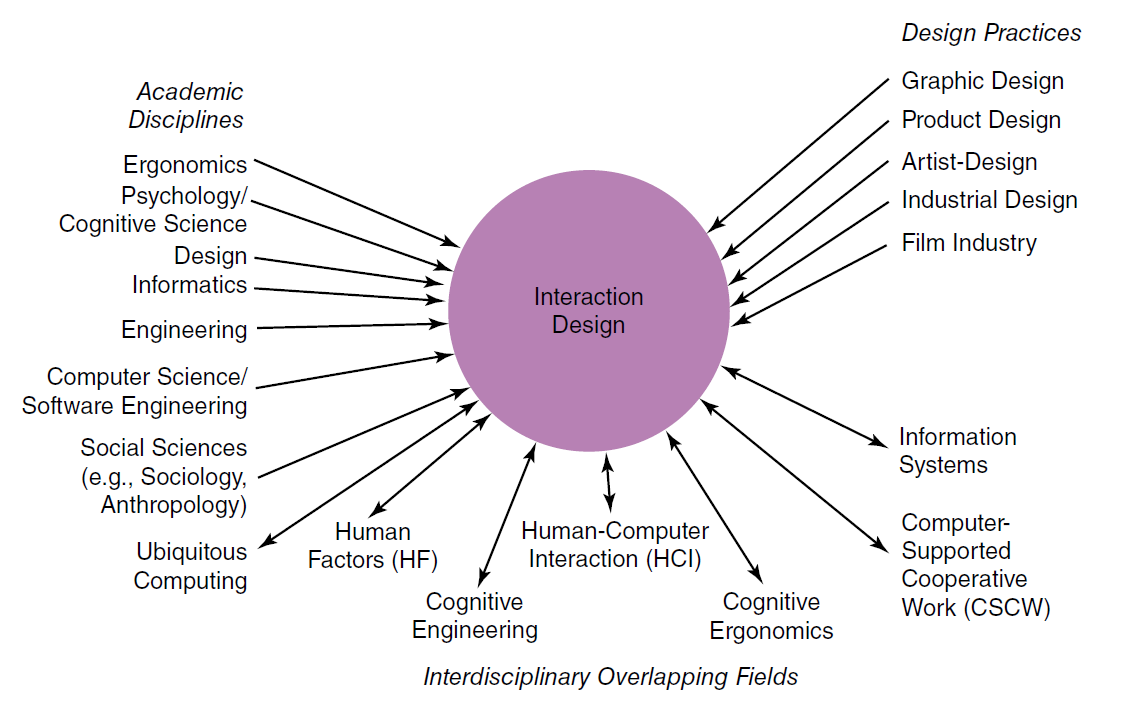
\includegraphics[width=\textwidth]{chapter-2-interaction-design.png}
  \caption{Hubungan studi antardisiplin terkait desain interaksi (Panah dua arah berarti saling tumpang tindih) (Sharp, dkk., 2019)}
  \label{fig:desain_interaksi}
\end{figure}

\subsection{Pendekatan Desain Interaksi}
\label{subsec:pendekatan_id}

Dalam desain interaksi terdapat beberapa pendekatan utama yang dapat digunakan untuk menyusun solusi permasalahan, yaitu \textit{user-centered design} (UCD), \textit{activity-centered design}, \textit{systems design}, dan \textit{genius design}. \parencite{saffer2010designing}

\begin{enumerate}
  \item \textit{User-Centered Design} (UCD)
  \subitem Konsep utama dari UCD adalah mendesain seputar kebutuhan penggunanya. Seorang desainer perlu mendefinisikan tujuan utama dari produk yang dibuat seputar apa yang ingin dicapai oleh penggunanya. Seringkali pengguna pun dilibatkan dalam tahap-tahap pengembangan, seperti pembuatan konsep, pengumpulan data, serta proses pengujian. Hal ini bertujuan untuk menjauhkan produk akhir dari preferensi desainer dan mendekatkan pada preferensi penggunanya sendiri.
   
  \item \textit{Activity-Centered Design}
  \subitem Berbeda dari UCD, pendekatan dengan \textit{activity-centered design} akan memfokuskan seputar kegiatan tertentu. Kegiatan yang dimaksud dapat didefinisikan sebagai kumpulan tugas yang dilakukan untuk mencapai tujuan tertentu. \textit{Activity-centered design} mengharuskan desainer untuk membuat solusi di seputar kegiatan dan menopang kegiatan tersebut, melainkan tujuan dari kegiatan tersebut. Desainer juga harus membedakan maksud dari sebuah aktivitas dengan tujuannya, di mana mereka harus menitikberatkan fokus desain pada maksud dari aktivitas.
 
  \item \textit{Systems Design}
  \subitem \textit{Systems design} adalah pendekatan yang memfokuskan permasalahan pada keseluruhan sebuah sistem dalam proses desainnya. Sistem yang dimaksud bisa terdiri dari banyak komponen pendukung seperti manusia, perangkat keras dan lunak, mesin, dan objek lain sehingga permasalahan yang dihadapi cenderung lebih kompleks.
 
  \item \textit{Genius Design}
  \subitem Pendekatan dengan \textit{Genius Design} mengandalkan sepenuhnya terhadap pengalaman, keahlian, serta preferensi dari desainernya sendiri dalam membuat keputusan desain. Keterlibatan pengguna sangat jarang dan biasanya hanya ada untuk memvalidasi apakah desain yang diprediksi sesuai dengan yang desainer inginkan. Pendekatan ini dinilai memiliki resiko-resiko yang cukup besar namun terkadang dilakukan karena alasan yang lebih kuat daripada resiko tersebut.
 
\end{enumerate}

\subsection{\textit{User-Centered Design} (UCD)}
Seperti yang telah dijelaskan pada subsubbab \ref{subsec:pendekatan_id}, pendekatan UCD memusatkan perhatian proses desain pada pengguna. UCD sendiri merupakan turunan dari cabang ilmu HCI (\textit{Human-Computer Interaction}), yaitu metodologi rekayasa perangkat lunak bagi pengembang yang ditujukan agar perangkat lunak dapat memenuhi kebutuhan penggunanya. \parencite{lowdermilk2013user} Namun pendekatan ini tidak semerta-merta menanyakan langsung keingingan pengguna untuk produknya, karena hal ini dapat membuat produk yang dibuat bias ke pihak tertentu. UCD memiliki tahap dan panduan di mana seorang desainer atau ahli UCD akan mengidentifikasi profil dari penggunanya serta perilaku dan preferensi terhadap aspek-aspek sebuah produk. Informasi yang didapat akan kemudian digunakan dalam proses desain. \parencite{10.1145/1621995.1621997}.

Dalam pendekatan UCD, seorang desainer juga tidak hanya membuat desain dengan tampilan antarmuka yang bagus. Desainer harus memastikan agar desain yang dibuatnya menyelesaikan permasalahan awal sesuai dengan riset yang telah dilakukan dan data yang telah diambil dari pengguna. Desainer bertanggung jawab untuk melakukan evaluasi dengan user untuk memastikan desain yang telah dibuatnya tepat sasaran. \parencite{lowdermilk2013user}

Dalam penerapannya, pendekatan UCD harus mengikuti prinsip-prinsip tertentu. Menurut \textcite{iso9241-210:2010}, berikut adalah prinsip-prinsip standar yang perlu diikuti:

\begin{enumerate}
  \item Desain dibuat berdasarkan pemahaman jelas atas pengguna, tugas-tugas, dan lingkungannya.
  \item Pengguna dilibatkan keseluruhan proses desain dan perkembangannya.
  \item Desain akan diubah dan diperbaiki secara terus-menerus sesuai dengan evaluasi dari pengguna.
  \item Proses UCD dilakukan secara berulang (iteratif).
  \item Desain meliputi keseluruhan \textit{user experience}.
  \item Pembuatan desain melibatkan berbagai perspektif dan kemampuan multidisipliner.
\end{enumerate}

\subsubsection{Proses-Proses dalam UCD}

Dalam melakukan perancangan desain dengan menerapkan pendekatan UCD, terdapat beberapa standar alur pekerjaan yang dapat diikuti. Salah satu yang umum digunakan adalah alur kerja standar ISO 9241-210. Berikut adalah alur kerja UCD sesuai dengan standar ISO 9241-210 yang tercantum pada Gambar II.2.

\begin{figure}[h]
  \centering
  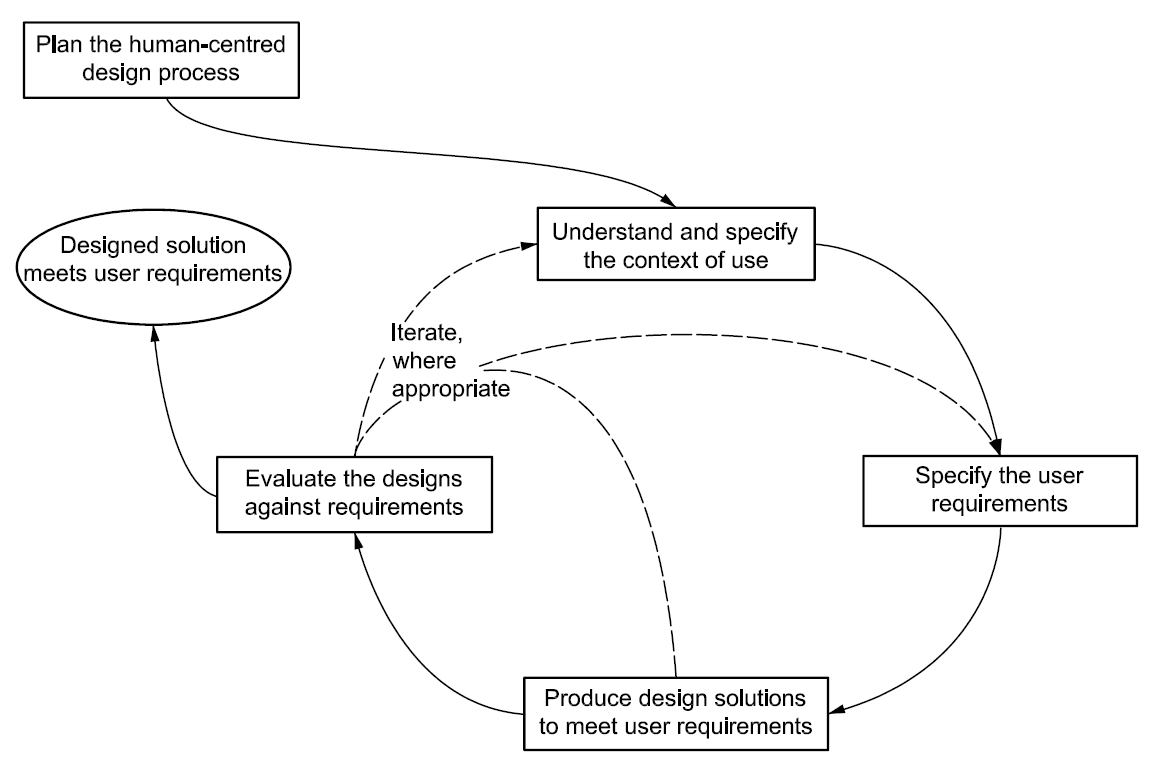
\includegraphics[width=0.9\textwidth]{chapter-2-ucd-figure.png}
  \caption{Alur kerja \textit{User-Centered Design} (\parencite{iso9241-210:2010})}
  \label{fig:diagram_iso2}
\end{figure}

Terlihat pada diagram alur kerja pada Gambar \ref{fig:diagram_iso2}, terdapat beberapa kegiatan yang dilakukan secara iteratif. Kegiatan-kegiatan yang dilakukan secara iteratif tersebut merupakan komponen utama dalam kerangka UCD. Berikut adalah penjelasan mengenai kegiatan-kegiatan tersebut:

\begin{enumerate}
  \item Memahami dan merincikan konteks penggunaan produk
  \subitem Pada tahap ini dilakukan pengumpulan dan analisa informasi mengenai konteks pemakaian produk. Hal ini bertujuan untuk mengungkapkan adanya kebutuhan, permasalahan, serta batasan dari produk yang penting untuk pengembangan solusi yang akan dibuat. Konteks pemakaian ini perlu mencakup informasi mengenai keseluruhan \textit{stakeholder}, karakteristik target pengguna, tujuan dan kegiatan dari pengguna, serta lingkungan di mana sistem akan dibuat atau dikembangkan. Jika UCD diterapkan pada produk yang sudah dibuat, maka beberapa informasi yang sudah tersedia dapat digunakan untuk melakukan modifikasi atau meningkatkan kualitas produk.
   
  \item Merincikan kebutuhan pengguna
  \subitem Pada tahap ini dilakukan identifikasi dan analisa lebih lanjut terhadap data-data yang telah dikumpulkan pada tahap sebelumnya. Dari hasil analisa akan didapatkan kebutuhan pengguna yang perlu dipenuhi dalam desain yang akan dibuat nanti. Kebutuhan pengguna yang didapat juga perlu mempertimbangkan batasan yang perlu diikuti sesuai dengan konteks pemakaian produk.
  
  \item Membuat solusi desain yang memenuhi kebutuhan pengguna
  \subitem Tahap selanjutnya adalah membuat prototipe desain sesuai dengan kebutuhan pengguna yang telah diidentifikasi pada fase sebelumnya. Prototipe desain yang dimaksud adalah produk implementasi desain aplikasi yang sudah menyerupai produk akhir, tanpa adanya implementasi unsur-unsur teknikal aplikasi tersebut. Hal ini bertujuan agar pengguna dapat memahami interaksi dan antarmuka dari desain aplikasi untuk dievaluasi pada tahap selanjutnya sebelum menjalani implementasi akhir.
  
  \item Mengevaluasi desain yang dibuat terhadap kebutuhan
  \subitem Proses evaluasi adalah proses untuk menentukan apakah desain aplikasi yang dibuat telah menyelesaikan permasalahan atau memenuhi kebutuhan yang diidentifikasi pada tahap-tahap sebelumnya. Proses evaluasi juga dilakukan untuk mengetahui apakah desain aplikasi sesuai dengan \textit{user experience goals} dan \textit{usability goals} yang diharapkan. Proses evaluasi tidak menutup kemungkinan adanya wawasan baru mengenai kebutuhan pengguna atau desain aplikasinya sendiri. Hasil dari evaluasi akan menentukan apakah desain tersebut layak dilanjutkan ke tahap implementasi atau diperlukan iterasi untuk menjalani perbaikan.

\end{enumerate}



\subsection{\textit{Usability Goals} dan \textit{User Experience Goals}}
Untuk mendesain produk yang tepat bagi pengguna, seorang desainer perlu mengerti kebutuhan pengguna dengan menentukan tujuan yang jelas dari pengembangan produk interaktif tersebut. \textcite{PreeceRogersSharp15} menyebutkan bahwa untuk mencapainya, tujuan dapat diklasifikasikan sesuai dengan \textit{usability goals} dan \textit{user experience goals}.

% http://bpm.umg.ac.id/aset/images/download/M4-Standar-Rujuka-BA(1-8-2017).pdf


\textit{Usability goals} mengarahkan produk untuk mencapai kriteria \textit{usability} tertentu. \textit{Usability goals} mencakup bagaimana cara untuk mengoptimalisasi interaksi pengguna dengan produk untuk melakukan kegiatannya. \textit{Usability goals} dapat diuraikan menjadi 6 tujuan berikut:
\begin{enumerate}
  \item Efektif untuk digunakan (\textit{effectiveness}) adalah tujuan yang menunjukkan apakah suatu produk sukses dalam menjalankan tugasnya.
  \item Efisien untuk digunakan (\textit{efficiency}) adalah tujuan yang menunjukkan bagaimana sebuah produk dapat membantu pengguna dalam mencapai tujuannya. Sebuah produk dapat dikatakan efisien jika penggunanya dapat melakukan suatu kegiatan dalam langkah-langkah yang sederhana dan tidak menuntut pengguna untuk mempelajari langkah-langkah tersebut terlalu lama.
  \item Aman untuk digunakan (\textit{safety}) adalah tujuan yang menunjukkan bagaimana sebuah produk dapat melindungi penggunanya dari situasi yang berbahaya atau tidak diinginkan, atau melakukan hal-hal yang bersifat destruktif. Tujuan ini dapat dicapai dengan meminimalisir resiko yang dapat ditemui pengguna atau memberikan opsi untuk membatalkan aksinya. Tujuan ini juga menunjukkan bagaimana sebuah produk membantu penggunanya mengeksplorasi produk secara percaya diri.
  \item Memiliki utilitas yang baik (\textit{utility}) adalah tujuan yang menunjukkan bagaimana sebuah produk menyediakan fungsionalitas yang baik untuk membantu pengguna melakukan hal yang dibutuhkan atau diinginkan.
  \item Mudah untuk dipelajari (\textit{learnability}) adalah tujuan yang menunjukkan seberapa mudah sebuah produk untuk dipelajari hingga pengguna dapat menggunakannya dengan benar.
  \item Mudah untuk mengingat penggunaan (\textit{memorability}) adalah tujuan yang menunjukkan seberapa mudah bagi pengguna untuk mengingat bagaimana cara menggunakan sebuah produk setelah mempelajarinya.
\end{enumerate}


\textit{User experience goals} lebih bersifat subjektif dibandingkan \textit{usability goals} karena mencakup berbagai jenis emosi dan pengalaman yang dirasakan oleh pengguna saat berinteraksi dengan produk. \textit{User experience goals} juga berhubungan erat dengan estetika dari produk. \textit{User experience goals} terdiri dari 2 jenis, yaitu tujuan yang diharapkan dan tujuan yang tidak diharapkan. \parencite{PreeceRogersSharp15} Pembagiannya dapat dilihat pada Tabel \ref{tab:ux_goals}.

\subsection{Tipe Interaksi}
\label{subsec:tipe_interaksi}

Dalam menyusun konsep desain, penentuan cara pengguna berinteraksi dengan produk / aplikasi akan didasarkan pada tipe interaksi dari desainnya. Menurut \textcite{PreeceRogersSharp15}, ada 5 tipe utama, yaitu \textit{instructing}, \textit{conversing}, \textit{manipulating}, \textit{exploring}, dan \textit{responding}. Menentukan tipe interaksi dari desain dapat membantu untuk menyusun model konseptual sebelum menentukan tipe antarmuka dari desainnya. Suatu sistem tidak terkekang dalam memiliki satu jenis tipe interaksi, pengguna dapat merasakan pengalaman yang berbeda di bagian-bagian sistem dengan tipe interaksinya masing-masing. Berikut adalah penjelasan tentang tipe-tipe interaksi.

\begin{enumerate}
  \item \textit{Instructing}
  \subitem Pada desain yang menerapkan tipe interaksi \textit{instructing} pengguna akan melakukan aktivitasnya dengan cara memberikan instruksi kepada sistem. Pengguna dapat memberikan instruksi dengan mengetikan perintah, memilih opsi dari menu, mengatakan perintahnya ke mikrofon, memberikan gestur, atau sesederhana menekan satu atau kombinasi tombol. Keuntungan dalam memilih tipe interaksi ini adalah kecepatan dan efisiensi interaksi, cocok untuk aksi yang perlu dilakukan berulang kali. Contoh kasus yang menggunakan tipe interaksi \textit{instructing} adalah sebuah \textit{vending machine}, di mana konsumen memilih makanan yang ingin dibeli baik dengan mengetikkan nomor label makanan.

  \item \textit{Conversing}
  \subitem Tipe interaksi \textit{conversing} berdasar pada konsep di mana pengguna akan melakukan percakapan dengan sistem. Sistem didesain untuk membalas pengguna sebagaimana manusia biasa akan menjawab, berbeda dengan tipe interaksi \textit{instructing} di mana sistem hanya menuruti perintah yang diberikan. Pengguna mampu mendapatkan saran, jawaban lebih pribadi, atau berdiskusi dengan sistem. Pada umumnya, sistem akan memanfaatkan teknologi voice-recognition, AI, atau teknologi berbasis natural-language lainnya dalam menerima input, dan menggunakan pembangkitan suara atau cukup kalimat tertulis untuk memberikan balasan. Tipe interaksi ini dapat ditemukan pada sistem penasehat, fasilitas bantuan, serta chatbot.
  
  \item \textit{Manipulating}
  \subitem Tipe interaksi \textit{manipulating} melibatkan tindakan memanipulasi sebuah objek layaknya di dunia nyata, seperti menggerakan (dragging), membuka, dan menutup. Pengguna juga dapat melakukan aksi yang mungkin tidak dapat dilakukan di dunia nyata, seperti stretching, shrinking, memperbesar, dan memperkecil objek. Tujuan yang ingin dicapai adalah untuk memberikan penguna perasaan senyata mungkin bahwa mereka sedang beinteraksi langsung dengan objek digital. Prinsip dari tipe interaksi ini adalah objek yang ada di layar tetap tampak selama pengguna memanipulasinya, dan memberikan feedback yang langsung ketika dimanipulasi untuk mempertahankan perasaan nyatanya. Walaupun tipe interaksi ini dapat membuat pengguna mudah berinteraksi dengan objek, terdapat beberapa aksi yang sebaiknya menggunakan tipe interaksi lain seperti \textit{instructing}. Contohnya adalah ketika memperbaiki typo yang berulang di suatu dokumen, melainkan mengubahnya dengan mencari dan menggantinya satu per satu, lebih baik untuk memberikan instruksi kepada sistem untuk mencari typo tersebut di seluruh dokumen dan langsung mengganti semuanya.
  
  \item \textit{Exploring}
  \subitem Sistem yang menggunakan tipe interaksi \textit{exploring} melibatkan penggunanya untuk bergerak di sebuah lingkungan baik virtual maupun fisik. Lingkungan sistem dapat mendeteksi ketika pengguna melakukan aksi tertentu dan memicu suatu peristiwa yang dapat dirasakan dan diinteraksi oleh pengguna. Lingkungan sistem tidak selalu harus berbentuk dunia virtual 3D, tetapi kebanyakan sistem yang mengadopsi tipe interaksi \textit{exploring} memiliki, seperti eksibisi virtual yang diakses menggunakan perangkat VR atau sebuah game.
  
  \item \textit{Responding}
  \subitem Sistem dengan tipe interaksi \textit{responding} akan menginisiasi interaksinya dengan memberikan, menunjukkan, atau mendeskripsikan sesuatu kepada pengguna, dan menunggu sebuah tanggapan. Interaksi yang diberikan sistem bergantung pada konteks yang sedang dialami pengguna atau dideteksi sistem.  Contohnya sebuah aplikasi dapat memberikan rekomendasi restoran yang berada di dekat pengguna ketika melewati suatu jalan, atau sebuah \textit{smartwatch} memberi notifikasi penggunanya sudah berhasil berjalan sebanyak 10.000 langkah. Tantangan desain yang menggunakan tipe interaksi ini adalah mengetahui kapan pengguna merasa informasi yang diberikan akan merasa berguna, dan menghindari interaksi yang dirasa dapat mengganggu pengguna.

\end{enumerate}

\RaggedLeft
\begin{footnotesize}
\begin{longtable}[c]{|>{\cbnormspacing}m{0.44\textwidth}|>{\cbnormspacing}m{0.49\textwidth}|}
  \caption{\textit{User experience goals} yang diharapkan dan tidak diharapkan}
  \label{tab:ux_goals} \\
  \hline \centering\textbf{\textit{User experience goals} yang diharapkan} & \textbf{\textit{User experience goals} yang tidak diharapkan} \\ \hline \endfirsthead
  \hline \centering\textbf{\textit{User experience goals} yang diharapkan} & \textbf{\textit{User experience goals} yang tidak diharapkan} \\ \hline \endhead
  
  \hline \endfoot
  
  1.	Satisfying              & 1.  Boring                  \\
  2.	Helpful                 & 2.  Unpleasant              \\
  3.	Fun                     & 3.  Frustrating             \\
  4.	Enjoyable               & 4.  Patronizing             \\
  5.	Motivating              & 5.  Making one feel guilty  \\
  6.	Provocative             & 6.  Making one feel stupid  \\
  7.	Engaging                & 7.  Annoying                \\
  8.	Challenging             & 8.  Cutesy                  \\
  9.	Surprising              & 9.  Childish                \\
  10.	Pleasurable             & 10. Gimmicky                \\
  11.	Enhancing sociability   &                             \\
  12.	Rewarding               &                             \\
  13.	Exciting                &                             \\
  14.	Supporting creativity   &                             \\
  15.	Emotionally fulfilling  &                             \\
  16.	Entertaining            &                             \\
  17.	Cognitively stimulating &                             \\
  18.	Experiencing flow       &                             \\
\end{longtable}
\end{footnotesize}
\justifying
\FloatBarrier


\section{Penelitian Terkait}
\label{sec:penelitian_terkait}

Untuk membantu menyusun Tugas Akhir ini, digunakan beberapa penelitian yang pernah dilakukan sebagai sumber referensi. Referensi berikut digunakan sebagai pertimbangan dalam penyusunan desain solusi, atau untuk mengerti konteks dari tema yang dibahas.

\subsection{Socialize}

Socialize adalah sebuah aplikasi yang dibuat untuk membantu penelitian tentang aplikasi yang menerapkan konsep-konsep dari Digital Wellbeing. Dalam penelitian yang berjudul “The Race Towards Digital Wellbeing: Issues and Opportunities”, \textcite{CHI2019SOCIALIZE} meneliti aplikasi-aplikasi berbeda yang berkaitan dengan konsep Digital Wellbeing untuk menemukan fitur-fitur yang umum ditemukan.

Dari 42 aplikasi yang diteliti, ditemukan dua fungsi paling utama dari aplikasi berkonsep Digital Wellbeing adalah melacak dan memvisualisasi data penggunaan serta melakukan intervensi untuk mengurangi ketergantungan. Dalam upaya pelacakan data, 57\% aplikasi memiliki fitur menampilkan semacam visualisasi ringkasan dari penggunaan \textit{smartphone} pengguna, dan 50\% dapat menampilkan penggunaan per aplikasi. Dalam menampilkan ringkasan, aplikasi biasanya menggunakan grafik untuk memberikan visualisasi data (60\% aplikasi) atau \textit{widgets} yang lebih mudah diakses pengguna dari homescreen \textit{smartphone} (38\%).

Untuk melakukan intervensi, aplikasi-aplikasi menyediakan fitur untuk memberikan batas waktu penggunaan pada aplikasi atau disebut app timer (31\%), fitur yang memblokir akses ke aplikasi (26\%) atau masuknya notifikasi (19\%), fitur yang membatasi waktu penggunaan \textit{smartphone} (26\%) atau memblokirnya secara keseluruhan (15\%), atau fitur untuk beristirahat dari \textit{smartphone}-nya secara sementara (15\%). Sebagai fitur tambahan, beberapa aplikasi membantu pengguna dengan memberikan kutipan motivasi (12\%) atau suatu jenis penghargaan jika berhasil menyelesaikan suatu tantangan terkait Digital Wellbeing. Informasi lebih lengkap dari penemuan Roffarello dan De Russis dapat dilihat pada Gambar \ref{img:ruf_table} dan Gambar \ref{img:ruf_chart}.

\begin{figure}[h]
  \centering
  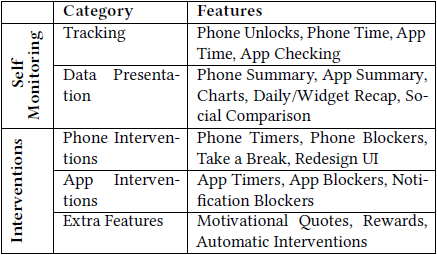
\includegraphics[width=0.5\textwidth]{chapter-2-ruf_table.png}
  \caption{Fitur-fitur umum pada aplikasi-aplikasi berkonsep Digital Wellbeing \parencite{CHI2019SOCIALIZE}}
  \label{img:ruf_table}
\end{figure}

\begin{figure}[h]
  \centering
  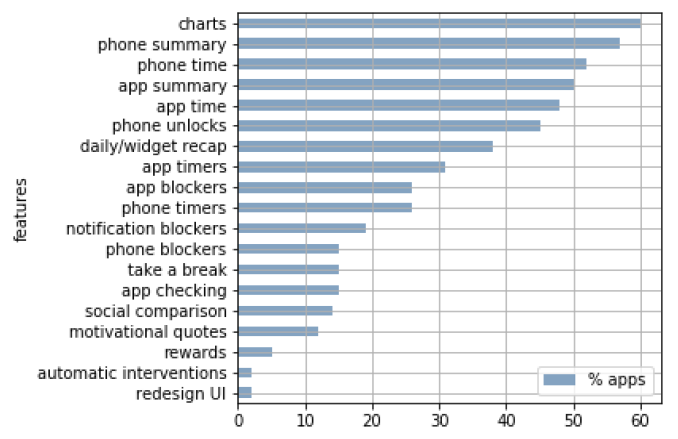
\includegraphics[width=0.7\textwidth]{chapter-2-ruf_chart.png}
  \caption{Distribusi fitur pada aplikasi-aplikasi berkonsep Digital Wellbeing \parencite{CHI2019SOCIALIZE}}
  \label{img:ruf_chart}
\end{figure}

Setelah melakukan penelitian terhadap fitur-fitur aplikasi, dilakukan pula analisis tematik terhadap 1.128 ulasan pengguna untuk aplikasi-aplikasi tersebut yang mencakup ulasan antara tahun 2015 dan 2018, baik ulasan positif maupun negatif. Hal ini dilakukan untuk mengetahui fitur apa saja yang disukai atau tidak oleh penggunanya. Roffarello dan De Russis menemukan bahwa banyak pengguna yang memang menyukai ide dari konsep Digital Wellbeing untuk memonitor dan memperbaiki kebiasaan penggunaan \textit{smartphone}, terbantu dengan mudahnya menggunakan aplikasinya. Pengguna menyukai banyaknya fitur yang tersedia, seperti pembatasan waktu dan pemblokiran akses, pelacakan dan statistik data, serta pemberian motivasi melalui penghargaan dan kutipan motivasi, dapat membantu memperbaiki kebiasaan penggunaan \textit{smartphone} atau kebiasaan lainnya secara efektif. Tak hanya itu, pengguna juga menemukan bahwa aplikasi sangat berguna untuk kasus penggunaan seperti pembatasan penggunaan \textit{smartphone} di saat belajar atau bekerja, pemantauan dan pengendalian perangkat milik anak kecil oleh orang tua, serta bantuan untuk memperbaiki jadwal tidur.

Di sisi lain, banyak pengguna yang mengeluhkan aplikasi-aplikasi kurang bersifat membatasi dan mudah untuk dikelabui, membuatnya tidak efektif dalam membatasi orang-orang yang kecanduan. Ada juga pengguna yang mengkhawatirkan tentang privasinya selama menggunakan fitur pelacakan, menilai aplikasi terasa intrusif. Selain itu, banyak ulasan pengguna yang mengeluhkan bug dan kecacatan desain hingga membuat aplikasi tidak berguna. Seluruh penemuan dirangkum menjadi kumpulan kata kunci yang dapat dilihat pada Gambar \ref{img:ruf_review}.

\begin{figure}[h]
  \centering
  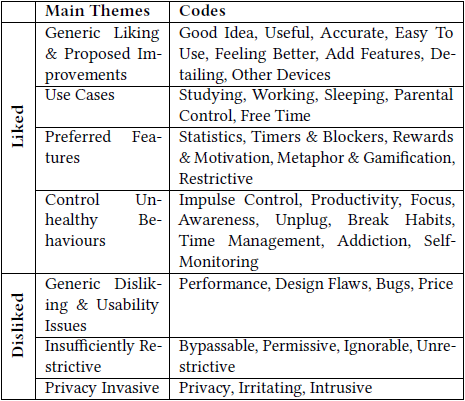
\includegraphics[width=0.5\textwidth]{chapter-2-ruf_review.png}
  \caption{Kata kunci pada analisis ulasan aplikasi-aplikasi berkonsep Digital Wellbeing \parencite{CHI2019SOCIALIZE}}
  \label{img:ruf_review}
\end{figure}

Dari analisis fitur umum dan ulasan, Roffarello dan De Russis membuat sebuah aplikasi Android bernama Socialize yang mencakup fitur-fitur paling umum dari aplikasi-aplikasi tersebut, yaitu fitur yang muncul pada setidaknya 15\% dari aplikasi-aplikasi yang dieksplorasi. Fitur-fitur yang diimplementasi dapat ditemukan pada Gambar \ref{img:ruf_fitur}, sedangkan tampilannya dapat dilihat pada Gambar \ref{img:ruf_app}. Lalu dilakukan pengujian aplikasi Socialize terhadap 38 orang untuk membandingkan penggunaan \textit{smartphone} sebelum dan sesudah memakai aplikasi. Secara kualitatif, ditemukan bahwa seluruh partisipan bersedia untuk menggunakan aplikasi Socialize lagi jika dirilis menjadi aplikasi sesungguhnya, dan memberikan masukan konstruktif tentang fitur-fiturnya. Beberapa partisipan juga antusias saat melihat statistik penggunaan \textit{smartphone}-nya. Partisipan juga mampu meningkatkan kualitas dari kebiasaan penggunaan \textit{smartphone}-nya dengan menggunakan fitur pembatasan dari Socialize. Namun di sisi lain, beberapa pengguna mengeluhkan bahwa Socialize membuat \textit{smartphone} mereka lebih boros dalam penggunaan baterai, atau mengganggu performa dari \textit{smartphone} mereka.

\begin{figure}[h]
  \centering
  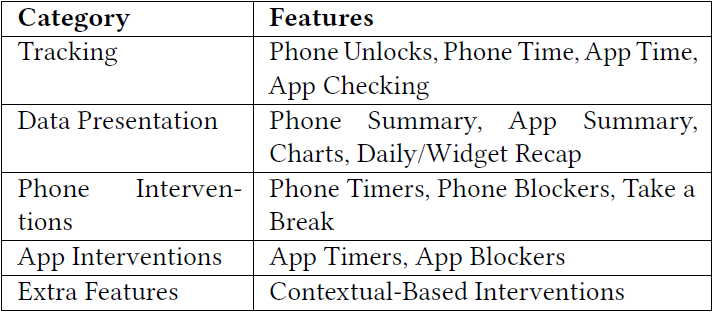
\includegraphics[width=0.55\textwidth]{chapter-2-ruf_fitur.png}
  \caption{Fitur-fitur yang diimplementasi pada aplikasi Socialize \parencite{CHI2019SOCIALIZE}}
  \label{img:ruf_fitur}
\end{figure}

\begin{figure}[h]
  \centering
  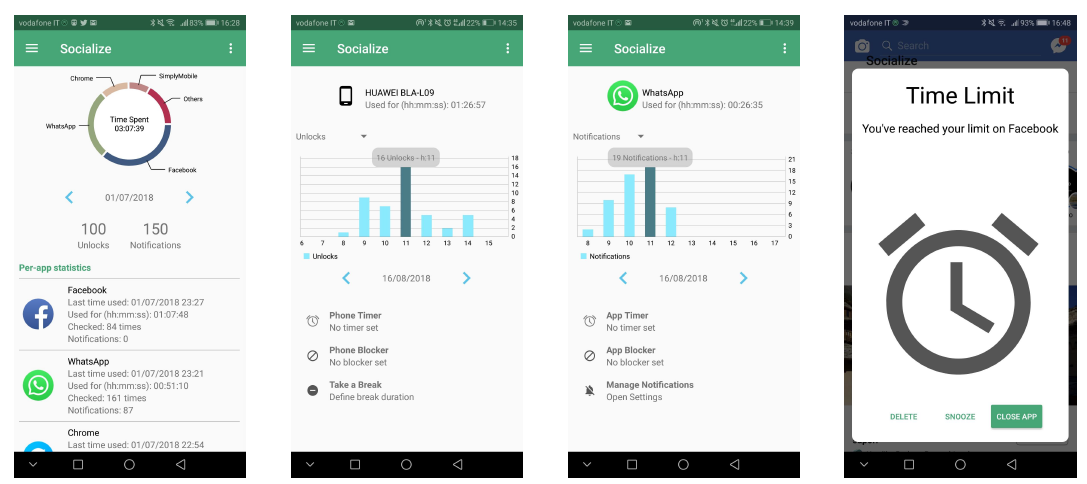
\includegraphics[width=\textwidth]{chapter-2-ruf_app.png}
  \caption{Tampilan aplikasi Socialize \parencite{CHI2019SOCIALIZE}}
  \label{img:ruf_app}
\end{figure}

Secara keseluruhan pada penelitian aplikasi Socialize, pengguna menyukai ide dari sebuah aplikasi Digital Wellbeing untuk membantu meningkatkan kualitas dari kebiasaan digitalnya. Namun solusi yang diberikan terkadang tidak cukup untuk menyelesaikan masalah yang ada. Masih perlu dibutuhkan tekad dari penggunanya untuk memanfaatkan fitur-fitur yang ada. Adapun beberapa masukan dari pengguna seperti kurang ketatnya pembatasan yang diberikan, dan diperlukannya interaksi sosial untuk membantu pengguna dalam mendapat bayangan dari kebiasaan digital yang baik. Penemuan yang cukup besar juga mengungkapkan bahwa aplikasi-aplikasi berkonsep Digital Wellbeing hanya membantu penggunanya dalam melakukan pemantauan mandiri dan menghentikan kebiasaan lama, tanpa membantu penggunanya mengembangkan kebiasaan baru yang lebih baik. Fitur yang dapat membantu hal tersebut, seperti pemberian kutipan motivasi dan penghargaan serta adanya interaksi sosial antarpengguna, cukup jarang ditemukan dari aplikasi-aplikasi Digital Wellbeing yang ada.

% \section{Usability Testing}
% Usability Testing adalah sebuah proses pengujian produk yang sedang dikembangkan untuk mengetahui apakah produk tersebut dapat digunakan dengan benar oleh pengguna yang terpilih, serta untuk menguji kepuasan pengguna dalam menggunakan produk. Dengan melakukan usability testing di sebuah lingkungan yang terkendali, desainer atau peneliti dapat mengendalikan pengaruh lingkungan yang dapat mempengaruhi performa pengguna. \parencite{PreeceRogersSharp15}

% Menurut \textcite{moran2019usabilitytest}, \textit{usability testing}, yang seringkali disebut juga \textit{user testing}, adalah suatu metodologi riset yang digunakan untuk mengidentifikasi masalah dalam sebuah desain produk atau layanan, menemukan celah atau ruang untuk perbaikan, serta mempelajari perilaku dan preferensi dari pengguna target produk. Dalam proses \textit{usability testing}, terdapat 3 elemen utama:
% \begin{enumerate}
%   \item Fasilitator
%   \subitem
%   Seorang fasilitator akan membimbing partisipan melalui proses pengujian, di mana dia akan memberikan instruksi-instruksi, menjawab pertanyaan partisipan, dan memberikan pertanyaan kepada partisipan. Fasilitator bertugas untuk memastikan bahwa data yang didapat dari pengujian memilki kualitas yang tinggi dan bersifat sah, tanpa mempengaruhi sikap dan tindakan pengguna saat mengerjakan pengujian.
  
%   \item Tugas
%   \subitem
%   Dalam melakukan pengujian, partisipan akan diberikan tugas-tugas realistis yang dapat dilakukan pada produk akhir di dunia nyata. Susunan kata pada tugas ini sangat penting, kesalahan penulisan atau pengguna frase dapat memberikan pengertian yang salah kepada pengguna dan dapat mempengaruhi sikap pengguna dalam menguji produk. 

%   \item	Partisipan
%   \subitem
%   Partisipan dari pengujian ini bermaksud sebagai pengguna realisitis yang masuk ke dalam target pemasaran produk, hal ini dapat berarti para partisipan memiliki latar belakang yang sama atau kebutuhan yang sama. Partisipan kemungkinan pernah memakai produknya, atau belum pernah sama sekali. Selama mengerjakan tugas, partisipan seringkali diperintahkan untuk mengatakan apa langkah yang sedang dilakukan untuk membantu penguji dalam mencatat data dan memastikan bahwa partisipan melakukan tugasnya sesuai dengan maksud penguji.
% \end{enumerate}

% \subsection{Sifat Usability Testing}
% Moran melanjutkan bahwa \textit{usability testing} memiliki sifat-sifat yang terbagi berdasarkan 2 kategori, yaitu:

% \begin{enumerate}
%   \item Data yang dikumpulkan
%   \subitem \textit{Usability testing} dapat dibagi berdasarkan data seperti apa yang ingin dikumpulkan. \textit{Qualitative usability testing} adalah pengujian yang berfokus untuk mengumpulkan wawasan dan temuan pengguna saat memakai produk. Pengujian ini cocok untuk menemukan masalah-masalah dalam pengalaman pengguna. \textit{Quantitative usability testing} adalah pengujian yang berfokus untuk mengumpulkan metrik yang digunakan untuk menjelaskan pengalaman pengguna. Metrik yang paling umum dikumpulkan adalah keberhasilan dan waktu pengerjaan tugas. Pengujian ini cocok untuk mengumpulkan tolok ukur.
  
%   \item Lokasi \textit{usability testing}
%   \subitem 
%   \textit{Usability testing} dapat dibagi berdasarkan lokasi pengguna dan pengamat saat melakukan pengujian. \textit{In-person usability testing} adalah pengujian di mana pengguna dan penguji berada di lokasi yang sama. Mereka tidak perlu berada di ruangan yang sama, namun pengamat dapat mengobservasi pengguna secara langsung. \textit{Remote usability testing} adalah pengujian di mana pengguna dan pengamat berada di lokasi yang berbeda. Pengujian ini lebih sering dipakai karena biayanya yang murah dan waktu yang diperlukan lebih singkat. Pengujian ini dapat dibagi lagi berdasarkan moderasi yang dilakukan selama pengujian berlangsung. Pada \textit{remote moderated usability testing} pengamat tetap mengobservasi pengguna namun melalui aplikasi konferensi online, sedangkan pada \textit{remote unmoderated usability testing} pengguna menggunakan kakas \textit{remote-testing} untuk mengerjakan tugas-tugas yang teWlah diberikan dan menanyakan pertanyaan lanjutan, kemudian rekaman sesi pengerjaan dan metrik yang didapat akan dikirim kepada penguji.
% \end{enumerate}

% \section{Keamanan Informasi}
% \textcite{andress2014basics} mengutip dari pemerintah Amerika Serikat, keamanan informasi adalah tindakan perlindungan informasi dan sistem informasi dari pengaksesan, penggunaan, penyingkapan, perubahan, dan pengrusakan yang tidak diizinkan. Andress meneruskan bahwa perlindungan yang dimaksud dapat terhadap serangan terhadap jaringan, bencana alam, kondisi lingkungan, kegagalan listrik, pencurian atau vandalisme, atau kondisi lainnya. Dalam sebuah usaha untuk melindungi informasi, dapat dipertimbangkan aset apa saja yang penting untuk diamankan, baik dari segi fisik maupun segi yang lebih rentan seperti perangkat lunak, kode, atau data.

% \subsection{Model Fundamental Keamanan Informasi}
% Terdapat model yang digunakan sebagai fundamental dalam merancang konsep keamanan informasi yang disebut sebagai CIA Triad. Kegagalan terhadap salah satu komponen dalam model CIA Triad dapat berarti kegagalan dalam keamanan informasi. Model CIA Triad terdiri dari Confidentiality, Integrity, dan Availability. \parencite{andress2014basics}
% \begin{figure}[h]
%   \centering
%   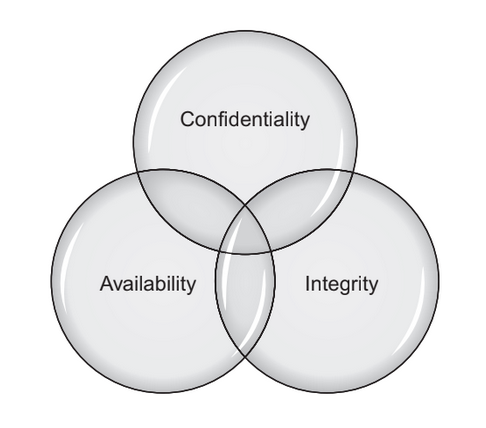
\includegraphics[width=0.5\textwidth]{chapter-2-model-CIA-triad.png}
%   \caption{Model CIA Triad}
% \end{figure}

% \begin{enumerate}[label=\alph*.]
%   \item \textit{Confidentiality}
%   \subitem 
%   \textit{Confidentiality} atau kerahasiaan adalah komponen penting dalam privasi yang berarti kemampuan sistem dalam melindungi data dari pihak yang tidak diizinkan. \textit{Confidentiality} dapat gagal ketika suatu pihak mendapatkan akses terhadap data yang dilindungi, misalnya dengan seseorang mengintip layar yang tertera data tersebut, atau data yang tidak sengaja dikirim lewat email kepada orang yang salah. 

%   \item \textit{Integrity}
%   \subitem
%   \textit{Integrity} atau integritas adalah kemampuan dalam mencegah data dari perubahan yang tidak diizinkan. Perubahan data yang dimaksud dapat berupa diubahnya atau dihapusnya sebagian atau seluruh data yang tidak diizinkan. \textit{Integrity} juga dapat gagal bila terjadi data diizinkan untuk diubah atau dihapus, namun tidak diinginkan. Hal ini berarti diperlukan sebuah mekanisme untuk membatalkan perubahan yang telah dilakukan selain mencegah dari perubahan yang tidak diinginkan.

%   \item \textit{Availability}
%   \subitem
%   \textit{Availability} atau ketersediaan adalah kemampuan untuk mengakses data ketika dibutuhkan. Kehilangan akses terhadap 1 buah data dapat merusak rantai pada sebuah sistem yang memerlukan akses terhadap data tersebut. Kegagalan terhadap \textit{availability} dapat terjadi karena kegagalan listrik, kegagalan sistem operasi, serangan jaringan, sistem yang tersusupi, atau masalah lain.

% \end{enumerate}

% \section{OWASP Top10}
% OWASP atau Open Web Application adalah sebuah komunitas terbuka yang berfokus pada keamanan di internet. OWASP mendedikasikan diri untuk memungkinkan organisasi-organisasi untuk mengembangkan, membeli, dan memelihara aplikasi dan API yang dapat dipercaya. Selain itu, OWASP membuat sebuah daftar 10 resiko kritis teratas yang dapat mengancam keamanan aplikasi web di internet, daftar ini disebut dengan OWASP Top10. Sejak tahun 2021, daftar ini terdiri atas:
% \begin{enumerate}
%   \item A01:2021 – Broken Access Control
%   \item A02-2021 – Cryptographic Failures
%   \item A03-2021 – Injection
%   \item A04-2021 – Insecure Design
%   \item A05-2021 – Security Misconfiguration
%   \item A06-2021 – Vulnerable and Outdated Components
%   \item A07-2021 – Identification and Authentification Failures
%   \item A08-2021 – Software and Data Integrity Failures
%   \item A09-2021 – Security Logging and Monitoring Failures
%   \item A10-2021 – Server-side Request Forgery (SSRF)
% \end{enumerate}

% \section{Privasi Informasi}
% Menurut Dr. Alan F. Westin yang dikutip oleh \textcite{givens2014information}, privasi sebuah klaim oleh individual, grup, atau institusi untuk menentukan sendiri kapan, bagaimana, dan sejauh apa informasi tentang mereka dapat dikomunikasikan kepada pihak lain. Givens meneruskan bahwa privasi informasi adalah subset dari pengertian privasi yang disebutkan oleh Westin. Givens mengutip Peter P. Swire dan Kenesa Ahmad bahwa ada 4 kelas dari privasi, yiatu privasi komunikasi, privasi wilayah, privasi tubuh, dan privasi informasi yang berarti perhatian terhadap pendirian ketentuan-ketentuan yang mengatur pengumpulan dan penanganan dari informasi pribadi, termasuk informasi medis dan finansial.

\chapter{Identifikasi Masalah dan Rancangan Solusi}

\newcommand{\ccnormspacing}{\baselineskip=12pt}
\newcommand{\ccnormspacingcenter}{\centering\arraybackslash\ccnormspacing}

Bab Identifikasi Masalah dan Rancangan Solusi berisi tentang penjelasan analisis permasalahan yang menjadi dasar dari tugas akhir ini. Secara garis besar, proses perancangan solusi akan mengikuti metodologi yang sudah ditetapkan yaitu pendekatan \textit{User-Centered Design} (UCD) menurut ISO 9241-210. Proses yang akan dibahas pada bab ini meliputi perancangan proses desain, identifikasi konteks penggunaan, analisis kebutuhan perangkat lunak, dan perancangan prototipe perangkat lunak. Gambaran alur UCD yang digunakan pada tugas akhir dapat dilihat pada Gambar \ref{fig:diagram_alur_kerja}.

\begin{figure}[h]
  \centering
  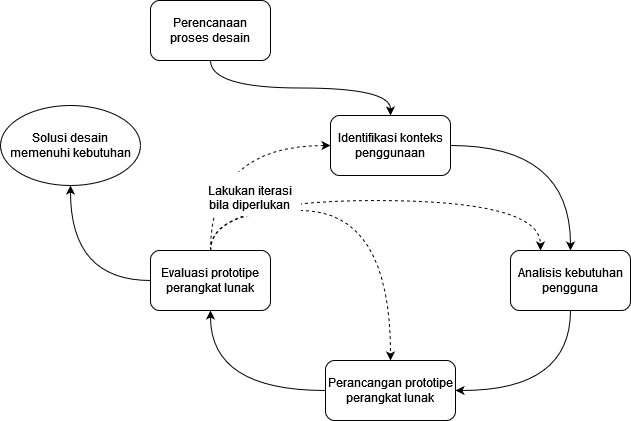
\includegraphics[width=0.8\textwidth]{chapter-1-method.png}
  \caption{Alur Kerja Penelitian}
  \label{fig:diagram_alur_kerja}
\end{figure}

\section{Perancangan Proses Desain}
\label{sec:perancangan_proses_desain}

Pada tahap perancangan proses desain dilakukan persiapan sumber daya yang diperlukan selama proses desain, serta penentuan ruang lingkup permasalahan.

% Sumber daya proses design

Ruang lingkup permasalahan yang ditentukan selama pengerjaan tugas akhir sebagai berikut

\begin{enumerate}
  \item Target Pengguna
  \subitem Target pengguna selama penelitian adalah pengguna \textit{smartphone} berbasis Android di Indonesia dengan rentang umur 18-34 tahun. Rentang usia tersebut adalah usia mayoritas pengguna media sosial di Indonesia. \parencite{mediasosial2020} 
  
  \item Fungsionalitas Aplikasi
  \subitem Lingkup fungsionalitas aplikasi adalah bagaimana desain interaksi yang baru dapat memperbaiki masalah yang ditemukan pada aplikasi Digital Wellbeing saat ini. Fungsionalitas dari aplikasi menyesuaikan dengan analisis hasil yang didapatkan dari riset dan wawancara. 
   
  \item Lingkup Pengembangan Aplikasi
  \subitem Desain interaksi aplikasi pencegah distraksi yang dibuat memiliki bentuk \textit{mobile interface} dengan mewujudkan sebuah prototipe aplikasi dalam \textit{platform Android}. Aplikasi Digital Wellbeing milik Google ditetapkan menjadi garis dasar pengembangan prototipe aplikasi tersebut.

\end{enumerate}

% * =======================================================================
% *   ||  ||  ||  ||  ||  ||  ||  ||  ||  ||  ||  ||  ||  ||  ||  ||  ||
% * =======================================================================


\section{Identifikasi Konteks Penggunaan}
\label{sec:identifikasi_konteks_penggunaan}

Pada tahap ini dilakukan proses analisis pengguna melalui data yang didapatkan dari ulasan pengguna aplikasi Digital Wellbeing dari situs Google Play Store, serta riset dengan metode wawancara. Kemudian akan dilakukan penyusunan persona pengguna dan pengidentifikasian fungsionalitas aplikasi yang akan membantu menentukan kebutuhan dan tujuan pengguna.

\subsection{Riset dan Analisis Pengguna}
\label{subsec:riset_analisis}

Tahap ini bertujuan untuk menganalis target pengguna, sehingga didapatkan data perilaku, masalah, tujuan, dan kebutuhan pengguna aplikasi Digital Wellbeing. Riset dilakukan dengan mengumpulkan data ulasan pengguna aplikasi Digital Wellbeing dari situs Google Play Store \textcite{dwplaystorereviews}. Metode pengumpulan data ini dipilih dengan alasan mengacu pada ISO 9241-210, bahwa informasi yang sudah tersedia dari suatu produk dapat dimanfaatkan untuk melakukan modifikasi atau peningkatan kualitas produk \parencite{iso9241-210:2010}, dalam hal ini informasi berbentuk ulasan pengguna.

Hasil terhadap analisis ulasan pengguna kemudian divalidasi dengan wawasan yang didapat dari wawancara. Karena pada data ulasan pengguna dari Google Play Store tidak terdapat informasi mengenai umur dan perilaku pengguna, wawancara dengan pengguna yang termasuk ke dalam lingkup permasalahan perlu dilakukan juga untuk mendapatkan wawasan mengenai perilaku pengguna. Perilaku pengguna berguna untuk menyusun persona pengguna.

\subsubsection{Ulasan Pengguna}
\label{subsubsec:ulasan_pengguna}

Berdasarkan situs Google Play Store per 13 April 2022, terdapat 609.005 ulasan untuk aplikasi Digital Wellbeing. Untuk menentukan jumlah \textit{sample size}, ditentukan \textit{confidence level} sebesar 95\%. Dikumpulkan data sebanyak 1000 ulasan dari target pengguna yang telah disebutkan pada bab \ref{sec:identifikasi_konteks_penggunaan},  kemudian dikategorikan secara manual, lalu didapatkan 288 ulasan yang dapat digunakan untuk menyusun masalah pengguna, sehingga \textit{sample} data memiliki \textit{margin of error} sebesar 5.78\%.

Pengkategorian ulasan dilakukan secara manual sehingga menghasilkan 11 kategori. Rincian tentang kategori tersebut dapat dilihat pada tabel \ref{tab:daftar_kategori}.

\RaggedLeft
\begin{small}
\begin{longtable}[c]{|W{c}{0.08\textwidth}|>{\ccnormspacing}m{0.72\textwidth}|>{\ccnormspacingcenter}m{0.1\textwidth}|}
  \caption{Daftar Kategori Ulasan}
  \label{tab:daftar_kategori} \\
  \hline \rowcolor[HTML]{A3E5F5} \textbf{ID} & \centering\textbf{Kategori Ulasan} & \textbf{Jumlah Ulasan} \\ \hline \endfirsthead
  \hline \rowcolor[HTML]{A3E5F5} \textbf{ID} & \centering\textbf{Kategori Ulasan} & \textbf{Jumlah Ulasan} \\ \hline \endhead
  
  \hline \endfoot
  
  KU-01    & Kurangnya widget untuk menampilkan data di Home Screen & 63 \\ \hline
  KU-02    & Perlu dikembangkannya fitur laporan penggunaan aplikasi untuk menampilkan data & 47 \\ \hline
  KU-03    & Perlu dikembangkannya fitur Focus Mode dengan menambah keketatan & 47 \\ \hline
  KU-04    & Perlu dikembangkannya kemampuan penjadwalan untuk fitur App Timer dan Focus Mode & 36 \\ \hline
  KU-05    & Kurangnya fitur pengaturan tingkat keketatan untuk fitur-fitur & 29 \\ \hline
  KU-06    & Kurangnya kemampuan penundaan untuk fitur App Timer & 18 \\ \hline
  KU-07    & Perlu dikembangkannya fitur Bedtime Mode dengan menambah keketatan & 12 \\ \hline
  KU-08    & Kurangnya penjelasan atau susunan kata yang dapat memotivasi pengguna untuk memakai fitur-fitur aplikasi & 12 \\ \hline
  KU-09    & Kurangnya fitur pengelompokkan aplikasi & 11 \\ \hline
  KU-10    & Kurangnya fitur pengaturan jam untuk akhir sebuah hari & 7 \\ \hline
  KU-11    & Kurangnya fitur \textit{whitelisting} untuk pembatasan akses aplikasi oleh Focus Mode & 6 \\ \hline
\end{longtable}
\end{small}
\justifying
\FloatBarrier

Adapun sejumlah ulasan yang tidak tergolong dalam kategori dinilai tidak relevan dalam penyusunan masalah pengguna, dengan penjelasan sebagai berikut

\begin{enumerate}
  \item Ulasan yang menilai positif aplikasi tanpa menyebutkan adanya masalah yang ditemukan dari aplikasi
  \item Ulasan yang menilai negatif aplikasi tanpa menyebutkan masalah yang ditemukan dari aplikasi
  \item Ulasan yang menyebutkan adanya bug dari aplikasi, seperti tidak berfungsinya sebuah fitur di perangkat tertentu
  \item Ulasan yang menyebutkan masalah yang tidak termasuk ke dalam batasan tugas akhir
  \item Ulasan yang tidak dapat dimengerti, seperti huruf-huruf yang tersusun secara acak 
  \item Ulasan yang melaporkan bahwa aplikasi tidak dapat dihapus dari perangkat
\end{enumerate}

\subsubsection{Perilaku Pengguna}
Setelah melakukan analisis ulasan pengguna untuk aplikasi Digital Wellbeing, dilakukan wawancara untuk mendapatkan perilaku pengguna, memvalidasi masalah pengguna dari analisis ulasan, serta menemukan masalah lain yang tidak ditemukan dari ulasan. Target berjumlah 5 orang dengan kriteria sebagaimana telah dijelaskan pada subbab \ref{sec:perancangan_proses_desain}. Jumlah tersebut dipilih karena menurut \textcite{nielsenusabilityproblems}, penelitian dengan 5 orang responden sudah cukup untuk menemukan rata-rata 85\% masalah dari desain sebuah produk, dan menambah responden lebih banyak akan mendapatkan wawasan tambahan yang semakin sedikit.

 Data perilaku responden digunakan untuk menyusun persona pengguna, serta membantu menganalisis kebutuhan pengguna terkait aplikasi Digital Wellbeing. Sedangkan hasil validasi ulasan pengguna digunakan untuk  menggali inti masalah yang dikeluhkan. Kedua pengamatan tersebut akan dibahas lebih lanjut dalam analisis masalah, kebutuhan, dan tujuan pengguna. Rancangan pertanyaan dapat dilihat pada Lampiran \ref{chpt:daftar_pertanyaan_wawancara}. Detail pemetaan pengamatan dengan pertanyaan wawancara dapat dilihat pada Tabel \ref{tab:pemetaan_pengamatan_wawancara}

\RaggedLeft
\begin{small}
\begin{longtable}[c]{|>{\ccnormspacing}m{0.72\textwidth}|p{0.2\textwidth}|}
  \caption{Pemetaan Pengamatan dengan Pertanyaan Wawancara}
  \label{tab:pemetaan_pengamatan_wawancara} \\
  \hline \rowcolor[HTML]{A3E5F5} \multicolumn{1}{|c|}{\textbf{Pengamatan}} & \multicolumn{1}{|c|}{\textbf{No. Pertanyaan}} \\ \hline \endfirsthead
  \hline \rowcolor[HTML]{A3E5F5} \multicolumn{1}{|c|}{\textbf{Pengamatan}} & \multicolumn{1}{|c|}{\textbf{No. Pertanyaan}} \\ \hline \endhead

  \hline \endfoot
  
  \rowcolor[HTML]{DCF3FC} \multicolumn{2}{|l|}{\textbf{A. Perilaku Responden}} \\ \hline
  Identitas responden & 1, 2, 3 \\ \hline
  Perilaku penggunaan \textit{smartphone} responden & 4, 5, 6, 7, 8 \\ \hline
  Perilaku responden terkait aplikasi pencegah distraksi & 9, 10, 11, 12 \\ \hline
  Perilaku responden terkait aplikasi \textit{Digital Wellbeing} & 13, 14, 15 \\ \hline
  \rowcolor[HTML]{DCF3FC} \multicolumn{2}{|l|}{\textbf{B. Validasi Ulasan Aplikasi Digital Wellbeing}} \\ \hline
  Validasi masalah kurangnya fitur widget pada Homescreen & 16, 17, 18 \\ \hline
  Validasi masalah pada fitur laporan data penggunaan aplikasi pada \textit{smartphone} & 19 \\ \hline
  Validasi masalah pada fitur Focus Mode & 20, 21 \\ \hline
  Validasi masalah untuk kemampuan penjadwalan pada fitur-fitur & 22, 23, 24 \\ \hline
  Validasi masalah kurangnya fitur pengaturan tingkat keketatan & 25, 26, 27 \\ \hline
  Validasi masalah kurangnya fitur penundaan pada App Timer & 28, 29, 30 \\ \hline
  Validasi masalah pada fitur Bedtime Mode & 31, 32, 33 \\ \hline
  Validasi masalah kurangnya penjelasan dan susunan kata & 34, 35 \\ \hline
  Validasi masalah kurangnya fitur pengelompokkan aplikasi & 36 \\ \hline
  Validasi masalah kurangnya fitur pengaturan jam akhir hari & 37 \\ \hline
  Validasi masalah kurangnya kemampuan \textit{whitelisting} & 38 \\ \hline
\end{longtable}
\end{small}
\justifying
\FloatBarrier

Jumlah responden yang diwawancarai adalah 10 (sepuluh) orang. Data hasil wawancara dapat dilihat pada Lampiran \ref{chpt:hasil_wawancara}. Dari 10 responden, 90\% mengakui tujuan utama dari penggunaan smartphone adalah berkomunikasi melalui aplikasi \textit{messenger}, dengan tujuan sekunder yaitu berinteraksi dengan media sosial atau sebagai sarana hiburan. Ditemukan bahwa 4 dari 10 orang menggunakan \textit{smartphone} sebagai alat utama yang membantu dalam pekerjaan, dengan tujuan untuk berkomunikasi dengan rekan atau klien, menggunakannya sebagai \textit{workstation}, atau mencari ide dan inspirasi.

Dari wawancara, ditemukan bahwa seluruh responden mengakui distraksi terkait dengan \textit{smartphone} lebih banyak berasal dari luar \textit{smartphone} itu sendiri, yaitu dari keinginan diri sendiri menggunakan \textit{smartphone} untuk memenuhi tujuan sekunder mereka. Walaupun hanya 30\% responden yang mengeluhkan notifikasi dari \textit{smartphone} dianggap mendistraksi mereka dari kegiatan utama, 70\% mengakui perlu untuk mencegah distraksi dari notifikasi dengan cara menggunakan aplikasi pencegah distraksi atau mengubah pengaturan notifikasi aplikasinya secara langsung.

Ditemukan juga bahwa rata-rata durasi penggunaan \textit{smartphone} harian keseluruhan responden adalah 6.2 jam per hari, di mana 70\% responden dapat menggunakan \textit{smartphone} selama lebih dari 6 jam sehari. Kedua angka tersebut melebihi rata-rata durasi penggunaan \textit{smartphone} di Indonesia pada tahun 2021 yaitu 5.4 jam per hari \parencite{dataai2022smartphoneindonesia}.  Keseluruhan dari responden menilai skala rata-rata 4 (empat) dari 5 (lima) terhadap durasi penggunaan \textit{smartphone} harian mereka. Di antara seluruh responden, 70\% mengakui butuh bantuan dari sebuah aplikasi pencegah distraksi untuk menurunkan durasi penggunaan tersebut.

Selain untuk mengurangi durasi penggunaan, responden juga memerlukan bantuan sebuah aplikasi untuk melakukan hal lain yang berhubungan dengan perbaikan kebiasaan digital mereka. Ditemukan 50\% responden memerlukan bantuan aplikasi untuk memantau penggunaan \textit{smartphone}, baik secara keseluruhan atau per aplikasi, dalam merencanakan perbaikan digital mereka. Lalu, 80\% dari responden merasa perlu diingatkan tentang tugas / kegiatan yang harus diselesaikan saat mereka menggunakan \textit{smartphone}. Keberadaan sebuah pengingat dapat menyadarkan pengguna terhadap alasan mereka menggunakan aplikasi pencegah distraksi. Selain itu, 50\% dari responden juga menggunakan aplikasi untuk membantu dalam memperbaiki jadwal tidurnya. Mereka mengakui bahwa saat menggunakan \textit{smartphone} sebelum tidur, seringkali mereka tidak menyadari waktu sehingga melewati jadwal tidur mereka.

Wawasan tentang perilaku pengguna yang didapat dapat disusun dalam bentuk variabel-variabel perilaku yang berguna dalam pembentukan persona. \textcite{cooper2014face} menyarankan bahwa dalam menyusun variabel dapat ditemukan perbedaan yang cukup jelas jika fokus kepada tipe-tipe variabel berikut
\begin{enumerate}
  \item Aktivitas, yaitu apa yang dilakukan pengguna dan seberapa sering 
  \item Sikap, yaitu pendapat pengguna tentang domain produk dan teknologi
  \item Kemampuan, yaitu bakat pengguna dan kemampuan untuk belajar
  \item Motivasi, yaitu alasan keterlibatan pengguna pada domain produk 
  \item Keterampilan, yaitu kemampuan pengguna terkait domain produk dan teknologi
\end{enumerate}

Keseluruhan variabel perilaku pengguna dirangkum pada Tabel \ref{tab:perilaku_pengguna}

\RaggedLeft
\begin{small}
\begin{longtable}[c]{|W{c}{0.06\textwidth}|>{\ccnormspacing}m{0.66\textwidth}|>{\ccnormspacingcenter}m{0.175\textwidth}|}
  \caption{Daftar Variabel Perilaku Pengguna}
  \label{tab:perilaku_pengguna} \\
  \hline \rowcolor[HTML]{A3E5F5} \textbf{ID} & \multicolumn{1}{|c|}{\textbf{Variabel Perilaku Pengguna}} & \multicolumn{1}{|c|}{\textbf{Tipe Perilaku}} \\ \hline \endfirsthead
  \hline \rowcolor[HTML]{A3E5F5} \textbf{ID} & \multicolumn{1}{|c|}{\textbf{Variabel Perilaku Pengguna}} & \multicolumn{1}{|c|}{\textbf{Tipe Perilaku}} \\ \hline \endhead
  
  \hline \endfoot
  
  P-01  &  Menggunakan \textit{smartphone} dengan tujuan primer untuk berkomunikasi melalui aplikasi \textit{messenger}  & Aktivitas \\ \hline
  P-02  &  Menggunakan \textit{smartphone} dengan tujuan primer untuk membantu dalam pekerjaan & Aktivitas \\ \hline
  P-03  &  Menggunakan \textit{smartphone} dengan tujuan sekunder untuk berinteraksi lewat media sosial & Aktivitas \\ \hline
  P-04  &  Menggunakan \textit{smartphone} dengan tujuan sekunder sebagai sarana hiburan & Aktivitas \\ \hline
  P-05  &  Menilai skala rata-rata 4 (empat) dari 5 (lima) terhadap durasi penggunaaan \textit{smartphone} harian & Aktivitas \\ \hline
  P-06  &  Merasa sering terdistraksi oleh keinginan diri sendiri untuk menggunakan \textit{smartphone}  & Sikap \\ \hline
  P-07  &  Merasa sering terdistraksi oleh notifikasi dari \textit{smartphone} & Sikap \\ \hline
  P-08  &  Merasa \textit{smartphone} sebaiknya membatasi pengguna seminimal mungkin & Sikap \\ \hline
  P-09  &  Merasa perlu ada sebuah penghargaan jika berhasil mengikuti jadwal pembatasan \textit{smartphone} & Sikap \\ \hline
  P-10  &  Mampu membatasi diri dari menggunakan \textit{smartphone} tanpa bantuan & Kemampuan \\ \hline
  P-11  &  Ingin memblokir notifikasi aplikasi yang dinilai sebagai distraksi & Motivasi \\ \hline
  P-12  &  Ingin mengurangi durasi penggunaan \textit{smartphone} harian & Motivasi \\ \hline
  P-13  &  Ingin memantau kebiasaan penggunaan \textit{smartphone} & Motivasi \\ \hline
  P-14  &  Ingin dibantu mengingatkan diri terhadap tugas / aktivitas yang harus dilakukan & Motivasi \\ \hline
  P-15  &  Ingin mengingatkan diri terhadap jadwal tidur & Motivasi \\ \hline
  P-16  &  Ingin diingatkan ketika terlalu lama menggunakan aplikasi & Motivasi \\ \hline
  P-17  &  Ingin memblokir akses ke aplikasi yang dinilai mendistraksi tanpa menghapusnya & Motivasi \\ \hline
  P-18  &  Mampu mengatur jadwal kegiatan dengan baik sehingga tidak mudah terdistraksi & Keterampilan \\ \hline
  P-19  &  Terbiasa dalam mengoperasikan aplikasi pencegah distraksi pada \textit{smartphone}  & Keterampilan \\ \hline
\end{longtable}
\end{small}
\justifying
\FloatBarrier

\subsubsection{Masalah Pengguna}
\label{subsubsec:masalah_pengguna}

Ditemukan bahwa kategori ulasan yang didapat dari analisis ulasan pengguna cukup bervariasi dengan jumlah yang tersebar. Namun, ulasan pengguna tidak cukup dalam menggambarkan inti dari masalah yang mereka alami. Tahap verifikasi dari wawancara membantu menemukan inti masalah yang dikeluhkan serta gambaran utama dari keseluruhan masalah tersebut. Pengguna mengeluhkan bahwa mereka kurang dapat mendapat gambaran tentang kebiasaan digital yang baik dari aplikasi Digital Wellbeing. Selain itu, pengguna juga kesulitan dalam menggunakan aplikasi Digital Wellbeing secara efisien untuk mencapai tujuan-tujuannya.

Untuk menyelesaikannya, masalah tersebut perlu dipecahkan menjadi masalah-masalah pengguna yang dapat dirincikan. Hal tersebut dilakukan untuk mempermudah penentuan kebutuhan dan tujuan pengguna serta penyusunan solusi. Keseluruhan masalah pengguna dirangkum pada Tabel \ref{tab:daftar_masalah}.

\RaggedLeft
\begin{small}
\begin{longtable}[c]{|W{c}{0.08\textwidth}|>{\ccnormspacing}m{0.6\textwidth}|>{\ccnormspacingcenter}m{0.2\textwidth}|}
  \caption{Daftar Masalah Pengguna}
  \label{tab:daftar_masalah} \\
  \hline \rowcolor[HTML]{A3E5F5}
  \textbf{ID} & \centering\textbf{Masalah Pengguna} & \textbf{Keterkaitan} \\ \hline \endfirsthead
  \hline \rowcolor[HTML]{A3E5F5}
  \textbf{ID} & \centering\textbf{Masalah Pengguna} & \textbf{Keterkaitan} \\ \hline \endhead

  \hline \endfoot

  MP-01  & Pengguna kesulitan dalam melakukan pengaturan fitur-fitur aplikasi Digital Wellbeing secara efisien & KU-01, KU-04, KU-05, KU-09, KU-10, KU-11 \\ \hline
  MP-02  & Pengguna kesulitan dalam menganalisis kebiasaan digital diri lewat aplikasi Digital Wellbeing & KU-02 \\ \hline
  MP-03  & Pengguna merasa fitur-fitur aplikasi Digital Wellbeing kurang ketat dalam membantu memperbaiki kebiasaan digital & KU-03, KU-04, KU-05, KU-06, KU-07 \\ \hline
  MP-04  & Pengguna merasa fitur-fitur aplikasi Digital Wellbeing kurang fleksibel & KU-04, KU-06, KU-09, KU-10 \\ \hline
  MP-05  & Pengguna merasa interaksi dengan aplikasi Digital Wellbeing kurang pribadi & KU-08 \\ \hline
  MP-06  & Pengguna kurang dapat memahami penggunaan fitur-fitur yang disediakan oleh aplikasi Digital Wellbeing & KU-08 \\ \hline
  MP-07  & Pengguna kesulitan dalam mengakses informasi pada fitur-fitur aplikasi Digital Wellbeing & KU-01 \\ \hline
\end{longtable}
\end{small}
\justifying
\FloatBarrier

% $ =====================================================
% $   +  +  +  +  +  +  +  +  +  +  +  +  +  +  +  +  +
% $ =====================================================


\subsection{Persona}
\label{subsec:persona_pengguna}
Setelah dilakukan analisis mengenai perilaku dan masalah pengguna, dilakukan segmentasi pengguna menjadi beberapa kelompok persona. Persona merepresentasikan kelompok-kelompok pengguna dengan karakteristik dan perilaku yang berbeda. Persona berperan menjadi arah pengembangan interaksi aplikasi dan mengurangi kemungkinan mendesain aplikasi untuk semua orang sehingga menghasilkan desain yang tidak disenangi oleh siapapun. \parencite{cooper2014face}

\subsubsection{Pengelompokkan Awal Pengguna}
Tahap awal dalam menyusun persona adalah mengelompokkan pengguna-pengguna berdasarkan perannya. Dari 10 orang partisipan riset wawancara, dikelompokkan menjadi 3 peran berdasarkan kemampuannya dalam membatasi diri dari smartphone tanpa membutuhkan bantuan. Kemampuan ini dianalisis dari data-data yang didapat melalui wawancara, semakin tinggi tingkat kemampuannya berarti pengguna tersebut dapat membatasi dirinya dengan bantuan sesedikit mungkin.

Terdapat pengguna dengan kemampuan tingkat rendah beranggotakan 20\% partisipan, pengguna berkemampuan tingkat sedang sebanyak 30\%, dan pengguna dengan tingkat tinggi sebanyak 50\%. Maka dari itu, pembagian untuk kelompok pengguna adalah sebagai berikut
\begin{enumerate}
  \item Kelompok 1: Pengguna yang sangat memerlukan bantuan untuk membatasi diri dari \textit{smartphone} 
  \item Kelompok 2: Pengguna yang memerlukan bantuan ringan untuk membatasi diri dari \textit{smartphone}
  \item Kelompok 3: Pengguna yang tidak memerlukan bantuan untuk membatasi diri dari \textit{smartphone}
\end{enumerate}

\subsubsection{Pemetaan Kelompok Pengguna dengan Variabel Perilaku}
Setelah dilakukan pengelompokkan pengguna, variabel-variabel perilaku yang telah diidentifikasi pada tahap riset dan analisis pengguna perlu dipetakan ke setiap kelompok pengguna. Hal ini bertujuan untuk mengidentifikasi perilaku dari setiap kelompok untuk kemudian disusun personanya.

Variabel perilaku yang dipetakan ke masing-masing kelompok pengguna akan memiliki jenis nilai yang berbeda. Variabel perilaku seperti P-01 dan P-02 menunjukkan apa saja nilai perilaku yang dipenuhi kelompok pengguna tersebut. Variabel perilaku seperti P-10 dan P-19 menunjukkan rentang atau tingkat perilaku dari kelompok pengguna tersebut. Sedangkan variabel perilaku seperti P-08 dan P-09 menunjukkan apakah pengguna memiliki perilaku tersebut. Hasil dari proses pemetaan dapat dilihat pada Tabel \ref{tab:pemetaan_perilaku}.

\RaggedLeft
\begin{small}
\begin{longtable}[c]{|>{\ccnormspacing}m{0.10\textwidth}|>{\ccnormspacing}m{0.31\textwidth}|>{\ccnormspacingcenter}m{0.145\textwidth}|>{\ccnormspacingcenter}m{0.145\textwidth}|>{\ccnormspacingcenter}m{0.145\textwidth}|}
  \caption{Daftar Pemetaan Kelompok Pengguna dengan Variabel Perilaku}
  \label{tab:pemetaan_perilaku} \\
  \hline \rowcolor[HTML]{A3E5F5}
  \centering\textbf{Variabel Perilaku} & \centering\textbf{Deskripsi Perilaku} & \textbf{Kelompok 1} & \textbf{Kelompok 2} & \textbf{Kelompok 3} \\ \hline \endfirsthead
  \hline \rowcolor[HTML]{A3E5F5}
  \centering\textbf{Variabel Perilaku} & \centering\textbf{Deskripsi Perilaku} & \textbf{Kelompok 1} & \textbf{Kelompok 2} & \textbf{Kelompok 3} \\ \hline \endhead

  \hline \endfoot

  \centering P-10  & Mampu membatasi diri dari menggunakan \textit{smartphone} tanpa bantuan & Rendah & Sedang & Tinggi \\ \hline
  \centering P-01 P-02  & Tujuan primer menggunakan \textit{smartphone} & Komunikasi & Pekerjaan, Komunikasi & Komunikasi, Pekerjaan \\ \hline
  \centering P-03 P-04 & Tujuan sekunder menggunakan \textit{smartphone} & Hiburan, Media sosial & Hiburan, Media sosial & Hiburan, Media sosial \\ \hline
  \centering P-05 & Penilaian durasi penggunaan \textit{smartphone} harian berdasarkan skala 1-5 & 5 & 4 & 3 \\ \hline
  \centering P-06 P-07 & Sumber distraksi terkait \textit{smartphone} & Keinginan diri sendiri, \textit{smartphone}, pihak lain & Keinginan diri sendiri, \textit{smartphone}, pihak lain & Keinginan diri sendiri \\ \hline
  \centering P-18 & Keterampilan dalam menyusun jadwal kegiatan & Rendah & Tinggi & Sedang \\ \hline
  \centering P-19 & Kebiasaan dalam menggunakan aplikasi pencegah distraksi & Tinggi & Sedang & Sedang \\ \hline
  \centering P-08 & Merasa \textit{smartphone} sebaiknya membatasi pengguna seminimal mungkin &   & \textbf{V} & \textbf{V} \\ \hline
  \centering P-09 & Merasa perlu ada sebuah penghargaan jika berhasil mengikuti jadwal pembatasan \textit{smartphone} & \textbf{V} &   &   \\ \hline
  \centering P-11 & Ingin memblokir notifikasi aplikasi yang dinilai sebagai distraksi & \textbf{V} & \textbf{V} & \textbf{V} \\ \hline
  \centering P-12 & Ingin mengurangi durasi penggunaan smartphone harian & \textbf{V} & \textbf{V} & \textbf{V} \\ \hline
  \centering P-13 & Ingin memantau kebiasaan penggunaan smartphone & \textbf{V} & \textbf{V} & \textbf{V} \\ \hline
  \centering P-14 & Ingin dibantu mengingatkan diri terhadap tugas / aktivitas yang harus dilakukan & \textbf{V} & \textbf{V} &   \\ \hline
  \centering P-15 & Ingin mengingatkan diri terhadap jadwal tidur & \textbf{V} & \textbf{V} &   \\ \hline
  \centering P-16 & Ingin diingatkan ketika terlalu lama menggunakan aplikasi & \textbf{V} &   &   \\ \hline
  \centering P-17 & Ingin memblokir akses ke aplikasi yang dinilai mendistraksi tanpa menghapusnya & \textbf{V} &   &   \\ \hline

\end{longtable}
\end{small}
\justifying
\FloatBarrier

\subsubsection{Pemetaan Kelompok Pengguna dengan Masalah Pengguna}
Selain variabel perilaku, masalah pengguna pun perlu dipetakan dengan kelompok pengguna yang telah dibuat. Hal ini dilakukan untuk mengenali masalah yang dirasakan oleh kelompok pengguna spesifik, dan juga membantu dalam menyusun persona.

Ditemukan bahwa ketiga kelompok pengguna mengalami sebagian besar dari masalah pengguna yang ada. Masalah pengguna MP-03 di mana aplikasi Digital Wellbeing dinilai kurang ketat tidak dirasakan oleh kelompok pengguna 3 karena tingginya kemampuan dalam membatasi diri dari smartphone tanpa membutuhkan bantuan. Di sisi lain, masalah MP-04 tentang fleksibilitas aplikasi tidak dirasakan oleh kelompok pengguna 1 karena perilakunya yang menunjukkan kebutuhan atas keketatan tinggi dari aplikasi dalam membatasi penggunaan smartphone. Selain itu, akibat keterampilan kelompok pengguna 1 dalam menggunakan aplikasi pencegah distraksi, mereka tidak mengalami masalah MP-06 karena mereka sudah cukup mengerti fitur-fitur yang digunakan. Hasil dari proses pemetaan dapat dilihat pada Tabel \ref{tab:pemetaan_masalah}.

\RaggedLeft
\begin{small}
\begin{longtable}[c]{|>{\ccnormspacing}m{0.08\textwidth}|>{\ccnormspacing}m{0.31\textwidth}|>{\ccnormspacingcenter}m{0.145\textwidth}|>{\ccnormspacingcenter}m{0.145\textwidth}|>{\ccnormspacingcenter}m{0.145\textwidth}|}
  \caption{Daftar Pemetaan Kelompok Pengguna dengan Masalah Pengguna}
  \label{tab:pemetaan_masalah} \\
  \hline \rowcolor[HTML]{A3E5F5}
  \centering\textbf{ID} & \centering\textbf{Deskripsi Masalah} & \textbf{Kelompok 1} & \textbf{Kelompok 2} & \textbf{Kelompok 3} \\ \hline \endfirsthead
  \hline \rowcolor[HTML]{A3E5F5}
  \centering\textbf{ID} & \centering\textbf{Deskripsi Masalah} & \textbf{Kelompok 1} & \textbf{Kelompok 2} & \textbf{Kelompok 3} \\ \hline \endhead

  \hline \endfoot

  \centering MP-01 & Pengguna kesulitan dalam melakukan pengaturan fitur-fitur aplikasi Digital Wellbeing secara efisien & \textbf{V} & \textbf{V} & \textbf{V} \\ \hline
  \centering MP-02 & Pengguna kesulitan dalam menganalisis kebiasaan digital diri lewat aplikasi Digital Wellbeing & \textbf{V} & \textbf{V} & \textbf{V} \\ \hline
  \centering MP-03 & Pengguna merasa fitur-fitur aplikasi Digital Wellbeing kurang ketat dalam membantu memperbaiki kebiasaan digital & \textbf{V} & \textbf{V} &  \\ \hline
  \centering MP-04 & Pengguna merasa fungsionalitas fitur-fitur aplikasi Digital Wellbeing kurang fleksibel &  & \textbf{V} & \textbf{V} \\ \hline
  \centering MP-05 & Pengguna merasa interaksi dengan aplikasi Digital Wellbeing kurang pribadi & \textbf{V} & \textbf{V} & \textbf{V} \\ \hline
  \centering MP-06 & Pengguna kurang dapat memahami penggunaan fitur-fitur yang disediakan oleh aplikasi Digital Wellbeing &  & \textbf{V} & \textbf{V} \\ \hline
  \centering MP-07 & Pengguna kesulitan dalam mengakses informasi pada fitur-fitur aplikasi Digital Wellbeing & \textbf{V} & \textbf{V} & \textbf{V} \\ \hline

\end{longtable}
\end{small}
\justifying
\FloatBarrier

\subsubsection{Penyusunan Karakteristik Persona}
Setelah dilakukan pemetaan kelompok pengguna terhadap variabel perilaku dan masalah, kelompok pengguna tersebut dapat disusun menjadi persona yang utuh dengan diberikan identitas dan karakter dalam bentuk sebuah narasi. Di dalam narasi tersebut, garis besar hasil pemetaan juga perlu disebutkan ulang. Hal-hal tersebut dapat membuat persona terasa hidup sehingga mempermudah proses penentuan kebutuhan dan tujuan pengguna, serta pembuatan solusi desain.

\newpage
Berikut adalah hasil penyusunan karakteristik persona untuk ketiga kelompok pengguna

\begin{enumerate}
  \item Persona 1: Nico
  \subitem Nico adalah seorang mahasiswa berumur 21 tahun yang sedang menjalani semester akhir di universitasnya. Nico mengerjakan tugas akhir pada laptopnya, namun ia merasa mudah terdistraksi oleh \textit{smartphone}nya, baik dari keinginannya untuk memeriksa media sosial atau permainan, maupun notifikasi yang sering muncul. Oleh karena itu, Nico menggunakan aplikasi Digital Wellbeing untuk memblokir akses ke aplikasi yang ia rasa mendistraksi serta mematikan notifikasinya. Namun terkadang Nico membuka blokirnya terlalu sering sehingga dia merasa adanya fitur dari Digital Wellbeing tidak berpengaruh dalam membantunya mencegah distraksi dari \textit{smartphone}-nya. Nico merasa butuh bantuan yang cukup besar dalam mengendalikan dirinya terkait \textit{smartphone} karena ia sering menyadari bahwa dirinya terlalu sering menggunakan \textit{smartphone}, melupakan tugasnya, dan jadwal tidurnya pun terganggu.

  \item Persona 2: Maya
  \subitem Maya adalah seorang pegawai swasta berumur 28 tahun. Dalam kesehariannya, Maya menggunakan \textit{smartphone} untuk berkomunikasi dengan rekan kerjanya, membantu dalam pekerjaannya, dan sebagai hiburan di jam istirahat. Maya sering terdistraksi di jam kerjanya oleh notifikasi atau keinginannya untuk memeriksa \textit{smartphone}, sehingga menggunakan aplikasi Digital Wellbeing untuk memblokirnya. Maya menemukan fitur-fitur menarik lain yang ia rasa dapat membantu mencegah distraksi, dan menganalisa serta memperbaiki kebiasaan penggunaan \textit{smartphone}nya. Namun Maya merasa bahwa beberapa fitur dari Digital Wellbeing kurang fleksibel untuk menyesuaikan dengan jadwal kerjanya yang bervariasi, seperti kurangnya kemampuan membuat jadwal lebih dari satu. Maya juga merasa pengalaman yang dirasakan kurang cukup personal untuk cukup memotivasinya karena pesan pengingat yang ia dapatkan terlalu membosankan.

  \item Persona 3: Nathan
  \subitem Nathan adalah seorang lulusan baru dan pekerja yang berumur 23 tahun. Dia terbiasa dalam mengatur jadwal pekerjaannya, dan sesekali menyelipkan jadwal untuk beristirahat. Ia melakukan sebagian besar pekerjaannya menggunakan \textit{smartphone}, seperti berkomunikasi, mengatur jadwal, dan menulis catatan. Nathan sesekali merasa bahwa dirinya memeriksa media sosial di \textit{smartphone} di waktu yang tidak tepat di saat jadwal kerjanya. Maka Nathan menggunakan fitur Focus Mode dari Digital Wellbeing untuk mengingatkan dirinya jika akan bermain \textit{smartphone} di jam kerjanya dan memblokir notifikasi dari aplikasi-aplikasi yang dianggap mendistraksi. Namun, Nathan tidak menggunakan fitur lain dari Digital Wellbeing karena ia merasa tidak perlu bantuan cukup banyak, tampilan dari aplikasi tidak cukup menarik, dan fitur-fitur yang ada tidak memiliki deskripsi yang jelas atau pengaturan yang cukup mudah.

\end{enumerate}

\subsubsection{Pemilihan Tipe Persona}
Dari persona-persona yang telah disusun, perlu dipilih sebuah persona primer. Persona primer akan dijadikan target utama atau panduan dalam membuat desain solusi. Persona primer yang dipilih harus dipertimbangkan agar tidak mengecewakan persona-persona lainnya. Dalam hal ini, persona 2, Maya, akan dijadikan sebagai persona primer. Namun dipilih juga persona 1, Nico, sebagai persona sekunder agar desain solusi yang dibuat tetap mampu memenuhi kebutuhannya.

Keputusan ini diambil melihat pertimbangan bahwa salah satu masalah terbesar dari aplikasi Digital Wellbeing adalah sulitnya pengguna dalam menggunakan aplikasi secara efisien untuk mencapai tujuan-tujuannya. Masalah tersebut tercerminkan dari masalah-masalah yang dikeluhkan oleh persona Maya dan persona lainnya. Dalam hal itu, solusi yang didesain untuk persona Maya diharapkan dapat menyelesaikan masalah-masalah yang dialami persona lain. Di sisi lain, kebutuhan persona Nico atas bantuan untuk membatasinya dari smartphone perlu dipertimbangkan dalam solusi desain, tanpa mengganggu desain yang ditujukan untuk persona primer.

% $ =====================================================
% $   +  +  +  +  +  +  +  +  +  +  +  +  +  +  +  +  +
% $ =====================================================


\subsection{Analisis Fungsionalitas Aplikasi}
\label{subsec:analisis_fungsionalitas}

% TODO lengkapin fungsionalitas aplikasi pencegah distraksi yang umum

Dalam mengidentifikasi konteks penggunaan produk, penting untuk mengerti lingkungan sistem dari produk tersebut. Fungsionalitas dari aplikasi Digital Wellbeing dapat langsung dari aplikasinya. Keseluruhan fungsionalitasnya dapat telah dijabarkan dalam Tabel \ref{tab:daftar_fungsionalitas_app_dw}.
% > Dalam mengidentifikasi konteks penggunaan produk, penting untuk mengerti lingkungan sistem dari produk tersebut. Untuk aplikasi Digital Wellbeing, perlu diidentifikasi fungsionalitas dari aplikasi pencegah distraksi pada umumnya untuk membantu mengidentifikasi kebutuhan pengguna. Dalam Tabel \ref{tab:daftar_fungsionalitas_app_dw} terdapat fungsionalitas dari aplikasi Digital Wellbeing yang sudah diterapkan.
% Sementara dalam Tabel \ref{daftar_fungsionalitas_app_umum} terdapat fungsionalitas yang belum diterapkan dalam aplikasi Digital Wellbeing yang ditemukan dalam aplikasi pencegah distraksi lain yang telah dipelajari sebagai bagian dari studi literatur Bab \ref{studi_kasus_aplikasi}.

\RaggedLeft
\begin{small}
\begin{longtable}[c]{|W{c}{0.08\textwidth}|>{\ccnormspacing}m{0.82\textwidth}|}
  \caption{Daftar Fungsionalitas Aplikasi Digital Wellbeing}
  \label{tab:daftar_fungsionalitas_app_dw} \\
  \hline \rowcolor[HTML]{A3E5F5} \textbf{ID} & \multicolumn{1}{|c|}{\textbf{Fungsionalitas}} \\ \hline \endfirsthead
  \hline \rowcolor[HTML]{A3E5F5} \textbf{ID} & \multicolumn{1}{|c|}{\textbf{Fungsionalitas}} \\ \hline \endhead
  
  \hline \endfoot
  
  FD-01  &  Aplikasi dapat melacak penggunaan harian dari \textit{smartphone} atau suatu aplikasi, dari sisi durasi penggunaan, jumlah pembukaan, dan notifikasi yang diterima \\ \hline
  FD-02  &  Aplikasi dapat menampilkan laporan penggunaan \textit{smartphone} atau suatu aplikasi dalam bentuk grafik dan daftar \\ \hline
  FD-03  &  Pengguna dapat menyetel batas waktu per hari akses suatu aplikasi \\ \hline
  FD-04  &  Aplikasi dapat memberikan notifikasi terkait batas waktu akses suatu aplikasi \\ \hline
  FD-05  &  Aplikasi dapat memblokir akses terhadap suatu aplikasi \\ \hline
  FD-06  &  Aplikasi dapat memblokir notifikasi yang dikirim suatu aplikasi \\ \hline
  FD-07  &  Pengguna dapat mengatur jadwal aktivasi pemblokiran akses untuk aplikasi yang dipilih \\ \hline
  FD-08  &  Pengguna dapat menunda pemblokiran akses sebuah aplikasi secara sementara \\ \hline
  FD-09  &  Pengguna dapat mengatur jadwal aktivasi mode waktu tidur \textit{smartphone} \\ \hline
  FD-10  &  Pengguna dapat menunda sementara aktivasi mode tidur \\ \hline
  FD-11  &  Pengguna dapat membuka pengaturan notifikasi aplikasi \\ \hline
\end{longtable}
\end{small}
\justifying
\FloatBarrier

\subsection{Analisis Kebutuhan dan Tujuan Pengguna}
\label{subsec:analisis_kebutuhan_tujuan}

Bagian dari identifikasi konteks penggunaan ini akan menganalisis tentang kebutuhan serta tujuan dari pengguna mengenai aplikasi Digital Wellbeing dan aplikasi pencegah distraksi secara umum, dibantu dengan data dari perilaku dan persona pengguna, masalah pengguna, dan fungsionalitas aplikasi. Keduanya akan berguna dalam merancang perbaikan desain interaksi yang diperlukan dari aplikasi Digital Wellbeing, terutama untuk menyusun \textit{usability goals} dan \textit{user experience goals}.

\subsubsection{Kebutuhan Pengguna}
\label{subsubsec:kebutuhan_pengguna}

Kebutuhan pengguna adalah hal apa saja yang diperlukan pengguna untuk mencapai tujuannya dalam memakai aplikasi Digital Wellbeing. Analisis kebutuhan pengguna melibatkan masalah pengguna serta perilaku pengguna yang telah dibahas sebelumnya. Penjelasan kebutuhan pengguna dirangkum di dalam Tabel \ref{tab:daftar_kebutuhan}.

\RaggedLeft
\begin{small}
\begin{longtable}[c]{|W{c}{0.07\textwidth}|>{\ccnormspacing}m{0.67\textwidth}|>{\ccnormspacingcenter}m{0.17\textwidth}|}
  \caption{Daftar Kebutuhan Pengguna}
  \label{tab:daftar_kebutuhan} \\
  \hline \rowcolor[HTML]{A3E5F5}
  \textbf{ID} & \centering\textbf{Kebutuhan Pengguna} & \textbf{Keterkaitan} \\ \hline \endfirsthead
  \hline \rowcolor[HTML]{A3E5F5}
  \textbf{ID} & \centering\textbf{Kebutuhan Pengguna} & \textbf{Keterkaitan} \\ \hline \endhead

  \hline \endfoot

  K-01  & Pengalaman pengaturan fitur yang lebih efisien dengan kemampuan seperti pencarian dan pengelompokan aplikasi & MP-01 \\ \hline
  K-02  & Widget untuk mengakses data serta melakukan pengaturan terhadap fitur-fitur lewat Homescreen & MP-01, MP-07 \\ \hline
  K-03  & Fitur rekomendasi untuk memberikan informasi tentang kebiasaan digital yang baik dan aksi yang dapat dilakukan & MP-02, P-05, P-06 \\ \hline
  K-04  & Laporan penggunaan \textit{smartphone} dengan rentang waktu lebih banyak dan ringkasan informasi seperti rata-rata penggunaan & MP-02, P-06 \\ \hline
  K-05  & Pengaturan tingkat keketatan untuk kemampuan tertentu dari fitur-fitur & MP-03, P-04 \\ \hline
  K-06  & Kemampuan penguncian pengaturan untuk mencegah pengubahan oleh pengguna & MP-03, P-04, P-05 \\ \hline
  K-07  & Fitur penjadwalan dengan kemampuan menambah lebih dari satu jadwal aktivasi fitur & MP-04, P-08 \\ \hline
  K-08  & Kemampuan penundaan pada restriksi yang diterapkan oleh fitur-fitur & MP-04 \\ \hline
  K-09  & Kemampuan pengaturan pesan untuk melakukan personalisasi pesan-pesan pengingat dari fitur-fitur & MP-05, P-07 \\ \hline
  K-10  & Tampilan aplikasi yang lebih menarik dengan deskripsi fitur yang lebih jelas & MP-06 \\ \hline
\end{longtable}
\end{small}
\justifying
\FloatBarrier

\subsubsection{Tujuan dan Kegiatan Pengguna}
\label{subsubsec:tujuan_kegiatan_pengguna}

Dengan ditentukannya kebutuhan pengguna, maka dapat dianalisis tujuan yang ingin dicapai oleh pengguna. Dalam mencapai tujuan-tujuan tersebut, maka perlu ditentukan kegiatan yang harus dilakukan oleh pengguna. Analisis tujuan dan kegiatan pengguna dilakukan dengan mengkaitkan kebutuhan pengguna dan perilaku pengguna. Hasil analisis dirangkum pada Tabel \ref{tab:daftar_tujuan_kegiatan}.

\newlength{\cccolgoal}
\setlength{\cccolgoal}{0.3\textwidth}

\newlength{\cccolneed}
\setlength{\cccolneed}{0.13\textwidth}

\newcommand{\ccgoal}[2]{\multirow{#1}{\cccolgoal}{\linespread{1}\selectfont #2}}
\newcommand{\ccneed}[2]{\multirow{#1}{\cccolneed}{\centering\linespread{1}\selectfont #2}}
\newcommand{\ccline}{\hhline{|-|~|-|~|}}


\RaggedLeft
\begin{small}
\begin{longtable}[c]{|W{c}{0.07\textwidth}|>{\ccnormspacing}m{\cccolgoal}|>{\ccnormspacing}m{0.38\textwidth}|>{\ccnormspacingcenter}m{\cccolneed}|}
  \caption{Daftar Tujuan dan Kegiatan Pengguna}
  \label{tab:daftar_tujuan_kegiatan} \\
  \hline \rowcolor[HTML]{A3E5F5}
  \textbf{ID} & \centering\textbf{Tujuan Pengguna} & \centering\textbf{Kegiatan Pengguna} & \textbf{Kebutuhan} \\ \hline \endfirsthead
  \hline \rowcolor[HTML]{A3E5F5}
  \textbf{ID} & \centering\textbf{Tujuan Pengguna} & \centering\textbf{Kegiatan Pengguna} & \textbf{Kebutuhan} \\ \hline \endhead

  \hline \endfoot

  UT-01 & & Mengunci pengaturan pada waktu tertentu & \\ \ccline
  UT-02 & & Membatasi istirahat yang dapat diambil pada fitur Focus Mode & \\ \ccline
  UT-03 & \ccgoal{-5}{Membatasi diri dari melonggarkan pengaturan} & Memilih tingkat keketatan dari fitur-fitur & \ccneed{-5}{P-03, K-05, K-06}\\ \hline
  
  UT-04 & & Membuat jadwal aktivasi fitur pemblokiran akses aplikasi & \\ \ccline
  UT-05 & \ccgoal{-3}{Mencegah distraksi dari smartphone di waktu tertentu} & Memilih aplikasi yang diblokir aksesnya & \ccneed{-3}{P-04, K-01, K-07}\\ \hline
  
  UT-06 & & Memasang batas waktu penggunaan harian aplikasi & \\ \ccline
  UT-07 & & Melihat sisa waktu penggunaan aplikasi lewat widget & \\ \ccline
  UT-08 & \ccgoal{-5}{Membatasi waktu penggunaan smartphone harian} & Melihat total waktu penggunaan smartphone lewat widget & \ccneed{-5}{P-05, K-02, K-01}\\ \hline
  
  UT-09 & & Mengakses laporan penggunaan smartphone & \\ \ccline
  UT-10 & & Memilih rentang waktu laporan penggunaan smartphone & \\ \ccline
  UT-11 & \ccgoal{-5}{Menganalisis kebiasaan penggunaan smartphone} & Melihat rekomendasi kebiasaan penggunaan smartphone yang baik & \ccneed{-5}{P-06, K-03, K-04}\\ \hline
  
  UT-12 & & Memasang pesan pengingat harian & \\ \ccline
  UT-13 & \ccgoal{-3}{Mengingatkan diri terhadap aktivitas utama yang seharusnya dilakukan} & Mengatur frekuensi notifikasi fitur pengingat  & \ccneed{-3}{P-07, K-09}\\ \hline
  
  UT-14 & & Mengatur jadwal aktivasi fitur Bedtime Mode & \\ \ccline
  UT-15 & \ccgoal{-3}{Membantu mengatur kebiasaan tidur yang sehat} & Membatasi aplikasi yang dapat diakses di jadwal tidur & \ccneed{-3}{P-08, K-05}\\ \hline
  
  UT-16 & & Mengambil waktu istirahat dari Focus Mode & \\ \ccline
  UT-17 & & Menunda aktivasi Bedtime Mode & \\ \ccline
  UT-18 & \ccgoal{-4}{Mengambil istirahat sejenak dari restriksi aplikasi} & Memperpanjang waktu penggunaan aplikasi yang diblokir oleh App Timer & \ccneed{-4}{K-08}\\ \hline

\end{longtable}
\end{small}
\justifying
\FloatBarrier

% * =======================================================================
% *   ||  ||  ||  ||  ||  ||  ||  ||  ||  ||  ||  ||  ||  ||  ||  ||  ||
% * =======================================================================



\section{Analisis Kebutuhan Perangkat Lunak}

% Proses perancangan solusi mengacu kepada metode \textit{User-Centered Design} sesuai dengan standar ISO 9241-210, di mana pada tahap perancangan desain interaksi untuk memenuhi kebutuhan pengguna akan disertai dengan prototipe aplikasi. Gambar \ref{fig:diagram_alur_kerja} menjelaskan tentang alur kerja penelitian yang dilakukan.

% \begin{figure}[h]
%   \centering
%   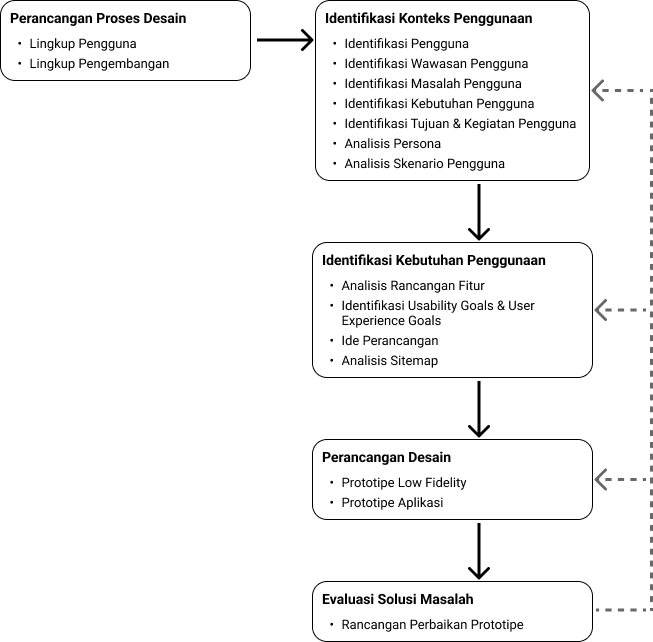
\includegraphics[width=0.8\textwidth]{chapter-3-alur-penelitian.png}
%   \caption{Alur Kerja Penelitian}
%   \label{fig:diagram_alur_kerja}
% \end{figure}

% \subsection{Perancangan Proses Desain}
% Ruang lingkup yang ditentukan pada penelitian ini adalah sebagai berikut

% \begin{enumerate}
%   \item Lingkup Pengguna
%   \subitem Target pengguna dari penelitian ini adalah masyarakat Indonesia yang pernah menggunakan atau memiliki ketertarikan terhadap aplikasi pencegah distraksi. Rentang usia dari target pengguna tidak dibatasi, namun difokuskan kepada golongan \textit{millenials} dengan rentang usia 18-30 tahun.
%   \item Lingkup Pengembangan
%   \subitem Desain interaksi aplikasi pencegah distraksi yang dibuat memiliki bentuk \textit{mobile interface} dengan mewujudkan sebuah prototipe aplikasi dalam \textit{platform Android}. Aplikasi Digital Wellbeing milik Google ditetapkan menjadi garis dasar pengembangan prototipe aplikasi tersebut.
% \end{enumerate}


% \subsection{Identifikasi Konteks Penggunaan}

% Pada tahap ini dilakukan analisis hasil riset penggunaanalisis terhadap hasil riset yang


% \subsection{Identifikasi Kebutuhan Pengguna}


% \subsection{Perancangan Desain}


% \subsection{Evaluasi Solusi Masalah}



% % Ketiga solusi yang telah diuraikan pada subbab \ref{sec:analisis_solusi} akan diimplementasikan dalam prototipe aplikasi, beserta fitur-fitur lain pada Digital Wellbeing yang akan mendukung solusi tersebut. Prototipe aplikasi ini akan diimpementasikan pada \textit{platform} Android. Secara garis besar, proses perancangan prototipe aplikasi akan menggunakan pendekatan \textit{user-centered design} (UCD).

% Seperti yang telah disebutkan pada subbab \ref{sec:metodologi}, metodologi yang digunakan dalam pengerjaan Tugas Akhir ini akan menggunakan pendekatan UCD. Dengan maksud mengikuti prosesnya, maka langkah selanjutnya yang akan dilakukan adalah mengumpulkan data. Pengumpulan data akan dilakukan dengan menyebarkan form secara online serta melakukan wawancara dengan responden yang bersedia untuk bekerja sama lebih lanjut. Proses ini akan dilaksanakan pada periode pengerjaan Tugas Akhir 2. Pengumpulan data ini bertujuan untuk melakukan validasi terhadap permasalahan yang sudah dianalisis, dan juga tidak menutup kemungkinan untuk menemukan permasalahan desain interaksi lain dari masukan pengguna.

% Setelah melakukan pengumpulan data, akan dilakukan analisis terhadap masukan yang didapat untuk mejadi kebutuhan perangkat lunak. Hasil analisis juga akan memvalidasi analisis masalah dan solusi yang didapat dari observasi penulis pada subbab \ref{sec:analisis_masalah} dan \ref{sec:analisis_solusi}.

% Kebutuhan perangkat lunak yang telah disusun akan diimplementasi dalam bentuk prototipe \textit{low-fidelity} terlebih dahulu. Setelah dilakukan evaluasi, maka implementasi akan dilanjutkan dalam bentuk prototipe \textit{high-fidelity}. Setelah menjalani evaluasi, maka perancangan prototipe aplikasi akan dikerjakan. Prototipe aplikasi diharapkan akan menghasilkan data dengan kualitas yang lebih tinggi pada saat evaluasi dibandingkan saat menggunakan prototipe \textit{low-fidelity} atau \textit{high-fidelity}. Hasil evaluasi juga akan menentukan apakah aplikasi akan menjalani proses iterasi atau diimplementasi lebih lanjut.

% \blindtext
\chapter{Implementasi dan Pengujian Prototipe}

Bab Implementasi dan Pengujian Prototipe berisi tentang lanjutan dari metodologi \textit{User-Centered Design}, yaitu tahap perancangan serta evaluasi prototipe perangkat lunak. Kedua tahap tersebut dilakukan iterasi sesuai dengan kebutuhan. Perancangan dan evaluasi akan dilakukan pada \textit{low-fidelity prototype} berbentuk \textit{wireframe} dan \textit{high-fidelity prototype} berbentuk prototipe \textit{mobile application} pada perangkat Android. Bagian perancangan prototipe menjelaskan tentang proses implementasi dari prototipe, sedangkan bagian evaluasi akan menjelaskan tentang proses pengujian prototipe yang berisi skenario dan hasil pengujian yang telah dicocokan dengan \textit{usability goals} dan \textit{user experience goals} yang sudah ditentukan sebelumnya. 

\section{Pengembangan Prototipe \textit{Low-Fidelity}}
\blindtext

\section{Pengujian Prototipe \textit{Low-Fidelity}}
\blindtext

\section{Pengembangan Prototipe \textit{High-Fidelity}}
\blindtext

\section{Pengujian Prototipe \textit{High-Fidelity}}
\blindtext
% \chapter{Kesimpulan dan Saran}

Bab Kesimpulan dan Saran menjelaskan tentang bagian akhir dari penelitian dan merupakan penutup dari laporan Tugas Akhir ini. Bab ini membahas tentang kesimpulan yang berisi ketercapaian tujuan penelitian terkait dengan rumusan masalah yang diselesaikan pada tugas akhir. Bab ini juga membahas tentang saran mengenai hal-hal yang dapat dilakukan untuk pengembangan selanjutnya.

\section{Kesimpulan}
Penelitian tugas akhir ini menghasilkan sebuah prototipe \textit{high-fidelity} aplikasi pencegah distraksi. Berdasarkan hasil analisis yang didapatkan, berikut adalah kesimpulan yang diambil

\begin{enumerate}
  \item Desain interaksi yang baik untuk sebuah aplikasi pencegah distraksi memprioritaskan \textit{usability goals} efisien untuk digunakan (\textit{efficiency}) dan mudah untuk dipelajari (\textit{learnability}), serta memiliki \textit{user experience goals} \textit{helpful} dan \textit{motivating}. Prototipe \textit{high-fidelity} aplikasi dinilai sudah baik dalam mencapai \textit{goals} tersebut, dilihat dari hasil analisis masukan pengguna pada \textit{usability testing}.
    \begin{enumerate}[label=\alph*.]
      \item Pengguna merasa bahwa aplikasi sudah cukup efisien untuk digunakan, melihat penilaian untuk metrik pengukuran \textit{System Usability Scale} (SUS) memiliki skor rata-rata 91,5 dari nilai maksimal 100, yang termasuk ke dalam kategori A atau di atas \textit{Excellent}. 
      
      \item Pengguna merasa bahwa aplikasi mudah untuk dipelajari, melihat penilaian untuk metrik pengukuran \textit{Single Ease Question} (SEQ) memiliki skor rata-rata 6,86 dari nilai maksimal 7.
      
      \item Pengguna merasa terbantu dalam menggunakan aplikasi, melihat penilaian untuk metrik pengukuran \textit{Intrinsic Motivation Inventory} (IMI) subskala \textit{Value/Usefulness} memiliki skor rata-rata 6,86 dari nilai maksimal 7.
      
      \item Pengguna merasa termotivasi dari menggunakan aplikasi, melihat penilaian untuk metrik pengukuran \textit{Intrinsic Motivation Inventory} (IMI) subskala \textit{Interest/Enjoyment} memiliki skor rata-rata 6,2 dari nilai maksimal 7, serta untuk subskala \textit{Pressure/Tension} memiliki skor rata-rata 1,36.
        
    \end{enumerate}
    
  \item kesimpulan
   
\end{enumerate}

\section{Saran}
Pada implementasi prototipe \textit{high-fidelity} aplikasi pencegah distraksi ini, masih banyak hal yang dapat ditingkatkan dan dikembangkan lebih lanjut. Maka dari itu, berikut adalah beberapa saran yang dapat dilakukan dalam pengembangan selanjutnya.

\begin{enumerate}
  \item Proses pengumpulan data untuk mengidentifikasi masalah pada tugas akhir ini masih menggunakan data dari ulasan aplikasi dari Google Play Store. Maka dari itu, pengumpulan data dapat ditingkatkan dengan melakukan penyebaran form kepada orang-orang yang termasuk ke dalam lingkup pengguna.
  \item Skenario pengujian dapat dilengkapi dengan menyertakan pengujian terhadap komponen-komponen yang hanya dapat diinteraksi dari prototipe aplikasi yang dapat berjalan, seperti notifikasi aplikasi serta pemblokiran penggunaan aplikasi yang dinilai mendistraksi.
\end{enumerate}

%----------------------------------------------------------------%

% Daftar pustaka
\printbibliography
% \blankpage

% Setting judul lampiran
\titlespacing*{\chapter}{0pt}{0pt}{0pt}
\titlespacing*{\section}{0pt}{0pt}{*1}

% Setting judul anak lampiran
\titleformat*{\section}{\bfseries}

% Index
\appendix
\chapter{Contoh Judul Lampiran}
\section{Contoh Judul Anak Lampiran}
Here is my appendix content...
\chapter{Analisis \textit{Web Scraping} Ulasan Pengguna Aplikasi Digital Wellbeing}
\label{chpt:web_scraping}

google-play-scraper versi 1.0.3 (\url{https://pypi.org/project/google-play-scraper/}).

\chapter{Daftar Pertanyaan Wawancara}
\label{chpt:daftar_pertanyaan_wawancara}

\newcommand{\apcsubrow}[1]{\rowcolor[HTML]{DCF3FC} \multicolumn{2}{|l|}{\textbf{#1}}}
\newcommand{\apcsubsubrow}[1]{\rowcolor[HTML]{E8E8E8} \multicolumn{2}{|l|}{\textbf{#1}}}

\RaggedLeft
% \label{tab:daftar_pertanyaan_wawancara}
\begin{footnotesize}
\begin{longtable}[c]{|p{0.04\textwidth}|>{\baselineskip=15pt}m{0.85\textwidth}|}
  \hline \rowcolor[HTML]{A3E5F5} \multicolumn{1}{|c|}{\textbf{No.}} & \multicolumn{1}{|c|}{\textbf{Pertanyaan}} \\ \hline \endfirsthead
  \hline \rowcolor[HTML]{A3E5F5} \multicolumn{1}{|c|}{\textbf{No.}} & \multicolumn{1}{|c|}{\textbf{Pertanyaan}} \\ \hline \endhead

  \hline \endfoot
  
  \apcsubrow{A. Perilaku Responden} \\ \hline
  
  \apcsubsubrow{Identitas Responden} \\ \hline
  1. & Jenis Kelamin Responden \\ \hline
  2. & Usia Responden \\ \hline
  3. & Pekerjaan Responden \\ \hline
  
  \apcsubsubrow{Perilaku Penggunaan \textit{Smartphone} Responden} \\ \hline
  4. & Apa tujuan responden dalam menggunakan \textit{smartphone}? (Diurutkan berdasarkan prioritas)  \\ \hline
  5. & Bentuk distraksi apa saja yang dialami terkait dengan smartphone?  \\ \hline
  6. & Seberapa sering responden menggunakan \textit{smartphone} dalam sehari? (Dalam hitungan jam)  \\ \hline
  7. & Dalam skala 1 sampai 5, dengan 1 sangat jarang dan 5 sangat sering, berapa Anda menilai jumlah penggunaan harian \textit{smartphone} Anda?  \\ \hline
  8. & Dalam skala 1 sampai 5, dengan 1 sangat sedikit dan 5 sangat banyak, berapa Anda menilai jumlah notifikasi yang diterima dari \textit{smartphone} Anda yang merupakan distraksi?  \\ \hline
  
  \apcsubsubrow{Perilaku Responden Terkait Aplikasi Pencegah Distraksi} \\ \hline
  9. & Apa nama aplikasi pencegah distraksi yang pernah Anda gunakan?  \\ \hline
  10. & Apa jenis fitur aplikasi pencegah distraksi yang ingin Anda gunakan?  \\ \hline
  11. & Masalah apa yang Anda temukan dari aplikasi pencegah distraksi yang pernah digunakan?  \\ \hline
  12. & Fitur atau kemampuan lain apa yang Anda inginkan dari sebuah aplikasi pencegah distraksi?  \\ \hline
  
  \apcsubsubrow{Perilaku Responden Terkait Aplikasi Digital Wellbeing} \\ \hline
  13. & Apa tujuan Anda dalam menggunakan aplikasi Digital Wellbeing?  \\ \hline
  14. & Masalah apa yang Anda temukan selama menggunakan aplikasi Digital Wellbeing?  \\ \hline
  15. & Fitur atau kemampuan lain apa yang Anda ingikan dari aplikasi Digital Wellbeing?  \\ \hline
  
  % ================================================
  
  \apcsubrow{B. Verifikasi Ulasan Aplikasi Digital Wellbeing} \\ \hline
  
  \apcsubsubrow{Verifikasi masalah kurangnya fitur widget pada Homescreen} \\ \hline
  16. & Bagaimana pendapat Anda tentang \textit{widget} yang menyediakan fungsionalitas dari fitur App Timer? \\ \hline
  17. & Bagaimana pendapat Anda tentang \textit{widget} yang menyediakan fungsionalitas dari fitur Focus Mode? \\ \hline
  18. & Bagaimana pendapat Anda tentang \textit{widget} yang menyediakan fungsionalitas dari fitur Bedtime Mode? \\ \hline
  
  \apcsubsubrow{Verifikasi masalah pada fitur laporan data penggunaan aplikasi} \\ \hline
  19. & Bagaimana pendapat Anda tentang pengembangan kemampuan dari grafik laporan pemakaian \textit{smartphone} atau aplikasi? \\ \hline
  
  \apcsubsubrow{Verifikasi masalah pada fitur Focus Mode} \\ \hline
  20. & Apakah Anda merasa fungsionalitas fitur Focus Mode pada \textit{notification bar} perlu dikembangkan dari segi keketatan? \\ \hline
  21. & Bagaimana pendapat Anda tentang fungsionalitas umum dari fitur Focus Mode dari segi keketatan? \\ \hline
  
  \apcsubsubrow{Verifikasi masalah untuk kemampuan penjadwalan pada fitur-fitur} \\ \hline
  22. & Bagaimana pendapat Anda tentang kemampuan untuk membuat jadwal lebih banyak untuk fitur App Timer? \\ \hline
  23. & Bagaimana pendapat Anda tentang kemampuan untuk membuat jadwal lebih banyak untuk fitur Focus Mode? \\ \hline
  24. & Bagaimana pendapat Anda tentang kemampuan untuk membuat jadwal App Timer yang berlangsung selama 1 minggu melainkan 1 hari? \\ \hline
  
  \apcsubsubrow{Verifikasi masalah kurangnya fitur pengaturan tingkat keketatan} \\ \hline
  25. & Bagaimana pendapat Anda tentang pengaturan untuk mengubah tingkat keketatan dari fitur-fitur dalam aplikasi? \\ \hline
  26. & Bagaimana pendapat Anda tentang kemampuan untuk mengunci pengaturan terhadap fitur-fitur? \\ \hline
  27. & Bagaimana pendapat Anda tentang mempersulit kemampuan untuk mengubah pengaturan terhadap fitur App Timer? \\ \hline
  
  
  \apcsubsubrow{Verifikasi masalah kurangnya fitur penundaan pada App Timer} \\ \hline
  28. & Bagaimana pendapat Anda tentang kemampuan \textit{reminder notification} terhadap sisa batas waktu dari aplikasi yang diatur oleh App Timer? \\ \hline
  29. & Bagaimana pendapat Anda tentang kemampuan untuk mengunci pengaturan terhadap fitur-fitur? \\ \hline
  30. & Bagaimana pendapat Anda tentang fitur indikator lama penggunaan aplikasi yang diatur dalam App Timer pada \textit{notification bar}? \\ \hline
  
  \apcsubsubrow{Verifikasi masalah pada fitur Bedtime Mode} \\ \hline
  31. & Bagaimana pendapat Anda tentang kemampuan untuk membatasi akses untuk aplikasi yang dipilih pengguna untuk mendukung fitur Bedtime Mode? \\ \hline
  32. & Bagaimana pendapat Anda tentang kemampuan untuk melarang perubahan jadwal jika fitur Bedtime Mode sedang aktif? \\ \hline
  33. & Bagaimana pendapat Anda tentang kemampuan untuk membatasi penundaan aktivasi fitur Bedtime Mode? \\ \hline
  
  \apcsubsubrow{Verifikasi masalah kurangnya penjelasan dan susunan kata} \\ \hline
  34. & Bagaimana pendapat Anda tentang kejelasan dalam deskripsi fitur-fitur aplikasi? \\ \hline
  35. & Bagaimana pendapat Anda tentang kemampuan untuk menambah pesan dalam \textit{reminder} yang diberikan oleh fitur-fitur? \\ \hline
  
  \apcsubsubrow{Verifikasi masalah kurangnya fitur pengelompokkan aplikasi} \\ \hline
  36. & Bagaimana pendapat Anda tentang kemampuan mengelompokkan aplikasi-aplikasi oleh pengguna untuk mempermudah pengaturan pada fitur Focus Mode atau App Timer? \\ \hline 
  
  \apcsubsubrow{Verifikasi masalah kurangnya fitur pengaturan jam akhir hari} \\ \hline
  37. & Bagaimana pendapat Anda tentang kemampuan untuk mengubah jam akhir dari sebuah hari? (Contoh: Mengubah akhir hari dari jam 12 malam menjadi jam 1 malam) \\ \hline
  
  \apcsubsubrow{Verifikasi masalah kurangnya kemampuan \textit{whitelisting}} \\ \hline
  38. & Bagaimana pendapat Anda tentang kemampuan untuk memilih aplikasi pada fitur Focus Mode dengan metode \textit{whitelisting}? \\ \hline
 
\end{longtable}
\end{footnotesize}
\justifying

\FloatBarrier
\chapter{Skenario Pengujian Prototipe \textit{Low-Fidelity}}
\label{chpt:skenario_lofi}

Setelah setiap pengerjaan skenario, partisipan akan diberikan pertanyaan mengenai skenario dan tugas yang telah mereka kerjakan. Pertanyaan ini berguna untuk mengevaluasi alur prototipe, informasi yang terdapat pada prototipe, serta mencari saran atau kritik dari partisipan. Pertanyaan-pertanyaannya adalah sebagai berikut

\begin{enumerate}
  \item Apa tanggapan Anda mengenai alur tampilan untuk menyelesaikan task tersebut?
  \item Apakah informasi pada tampilan cukup untuk membantu menyelesaikan task tersebut?
  \item Apakah ada masukan / saran mengenai tampilan dari halaman yang dilalui?
\end{enumerate}

\RaggedLeft
\begin{small}
\begin{longtable}[c]{|>{\ccnormspacing}m{0.19\textwidth}|>{\ccnormspacing}p{0.73\textwidth}|}
  
  \hline
  \rowcolor[HTML]{A3E5F5} \multicolumn{2}{|l|}{\textbf{Skenario Pengujian 1}} \\ \hline
  Kaitan Skenario Pengguna & SP-02 \\ \hline
  Tujuan & Mengukur pemahaman pengguna dalam menganalisis data penggunaan \textit{smartphone} \\ \hline
  Skenario & Pengguna ingin melihat data penggunaan \textit{smartphone} harian secara keseluruhan. \\ \hline
  Task & Lihat data penggunaan \textit{smartphone} \\ \hline
  Pra kondisi & Pengguna berada di Halaman Main Menu \\ \hline

  \rowcolor[HTML]{A3E5F5} \multicolumn{2}{|l|}{\textbf{Skenario Pengujian 2}} \\ \hline
  Kaitan Skenario Pengguna & SP-03 \\ \hline
  Tujuan & Mengukur pemahaman pengguna dalam membuat sebuah App Group \\ \hline
  Skenario & Pengguna ingin mengelompokkan aplikasi-aplikasi ke dalam sebuah grup. \\ \hline
  Task & Kelompokan aplikasi-aplikasi ke dalam sebuah kategori \\ \hline
  Pra kondisi & Pengguna berada di Halaman Dashboard \\ \hline

  \rowcolor[HTML]{A3E5F5} \multicolumn{2}{|l|}{\textbf{Skenario Pengujian 3}} \\ \hline
  Kaitan Skenario Pengguna & SP-02 \\ \hline
  Tujuan & Mengukur pemahaman pengguna dalam menganalisis data penggunaan satu buah aplikasi \\ \hline
  Skenario & Pengguna sudah melihat data penggunaan smartphone. Pengguna ingin melihat data penggunaan untuk hanya sebuah aplikasi. \\ \hline
  Task & Lihat data penggunaan dari sebuah aplikasi \\ \hline
  Pra kondisi & Pengguna berada di Halaman Dashboard \\ \hline

  \rowcolor[HTML]{A3E5F5} \multicolumn{2}{|l|}{\textbf{Skenario Pengujian 4}} \\ \hline
  Kaitan Skenario Pengguna & SP-02 \\ \hline
  Tujuan & Mengukur pemahaman pengguna dalam menganalisis data penggunaan App Group \\ \hline
  Skenario & Pengguna ingin melihat data penggunaan App Group yang sudah dibuat. \\ \hline
  Task & Lihat data penggunaan dari kategori aplikasi yang sudah dibuat \\ \hline
  Pra kondisi & Pengguna berada di Halaman Dashboard \\ \hline

  \rowcolor[HTML]{A3E5F5} \multicolumn{2}{|l|}{\textbf{Skenario Pengujian 5}} \\ \hline
  Kaitan Skenario Pengguna & SP-03 \\ \hline
  Tujuan & Mengukur pemahaman pengguna dalam memasang App Timer pada sebuah aplikasi \\ \hline
  Skenario & Pengguna ingin membatasi waktu penggunaan sebuah aplikasi. \\ \hline
  Task & Batasi waktu penggunaan dari sebuah aplikasi \\ \hline
  Pra kondisi & Pengguna berada di Halaman Main Menu \\ \hline

  \rowcolor[HTML]{A3E5F5} \multicolumn{2}{|l|}{\textbf{Skenario Pengujian 6}} \\ \hline
  Kaitan Skenario Pengguna & SP-05 \\ \hline
  Tujuan & Mengukur pemahaman pengguna dalam menunda aktivasi App Timer \\ \hline
  Skenario & Pengguna butuh waktu tambahan untuk menggunakan aplikasi yang batas waktunya telah habis. \\ \hline
  Task & Tunda pemblokiran untuk aplikasi yang batas waktu penggunaannya sudah habis \\ \hline
  Pra kondisi & Pengguna berada di Halaman Main Menu \\ \hline

  \rowcolor[HTML]{A3E5F5} \multicolumn{2}{|l|}{\textbf{Skenario Pengujian 7}} \\ \hline
  Kaitan Skenario Pengguna & SP-04 \\ \hline
  Tujuan & Mengukur pemahaman pengguna dalam menambah jadwal Focus Mode \\ \hline
  Skenario & Pengguna ingin fokus pada pekerjaannya di jam kerja. Pengguna ingin memblokir beberapa aplikasi di jam kerjanya. \\ \hline
  Task & Buat jadwal pemblokiran aplikasi-aplikasi mendistraksi sesuai dengan jam kerja \\ \hline
  Pra kondisi & Pengguna berada di Halaman Main Menu \\ \hline

  \rowcolor[HTML]{A3E5F5} \multicolumn{2}{|l|}{\textbf{Skenario Pengujian 8}} \\ \hline
  Kaitan Skenario Pengguna & SP-05 \\ \hline
  Tujuan & Mengukur pemahaman pengguna dalam menunda aktivasi Fokus Mode \\ \hline
  Skenario & Pengguna ingin beristirahat dari kerjanya sejenak. Pengguna ingin menggunakan aplikasi yang diblokir secara sementara. \\ \hline
  Task & Tunda pemblokiran aplikasi yang sudah dipasang sebelumnya \\ \hline
  Pra kondisi & Pengguna berada di Halaman Main Menu \\ \hline
  
  \rowcolor[HTML]{A3E5F5} \multicolumn{2}{|l|}{\textbf{Skenario Pengujian 9}} \\ \hline
  Kaitan Skenario Pengguna & SP-01 \\ \hline
  Tujuan & Mengukur pemahaman pengguna dalam menentukan Daily Goal \\ \hline
  Skenario & Pengguna memiliki sebuah target yang harus dipenuhi hari ini. Pengguna ingin mengingatkan diri terhadap capaian tersebut. \\ \hline
  Task & Pasang pengingat untuk capaian yang harus dipenuhi hari ini \\ \hline
  Pra kondisi & Pengguna berada di Halaman Main Menu \\ \hline
  
  \rowcolor[HTML]{A3E5F5} \multicolumn{2}{|l|}{\textbf{Skenario Pengujian 10}} \\ \hline
  Kaitan Skenario Pengguna & SP-01 \\ \hline
  Tujuan & Mengukur pemahaman pengguna dalam memanfaatkan Smartphone Usage Evaluation \\ \hline
  Skenario & Pengguna ingin diberikan evaluasi harian tentang penggunaan \textit{smartphone}-nya pada hari tersebut. \\ \hline
  Task & Pasang pengingat di akhir hari untuk memberikan evaluasi penggunaan \textit{smartphone} dan goal yang telah ditentukan \\ \hline
  Pra kondisi & Pengguna berada di Halaman Daily Goal \\ \hline
  
  \rowcolor[HTML]{A3E5F5} \multicolumn{2}{|l|}{\textbf{Skenario Pengujian 11}} \\ \hline
  Kaitan Skenario Pengguna & SP-06 \\ \hline
  Tujuan & Mengukur pemahaman pengguna dalam mengatur jadwal Bedtime Mode \\ \hline
  Skenario & Pengguna ingin memperbaiki jam tidurnya. Pengguna ingin mengurangi penggunaan \textit{smartphone} di saat jam tidur. \\ \hline
  Task & Aturlah sebuah jadwal agar \textit{smartphone} dapat masuk ke mode tidur di saat jam tidur. \\ \hline
  Pra kondisi & Pengguna berada di Halaman Main Menu \\ \hline

  \rowcolor[HTML]{A3E5F5} \multicolumn{2}{|l|}{\textbf{Skenario Pengujian 12}} \\ \hline
  Kaitan Skenario Pengguna & SP-02 \\ \hline
  Tujuan & Mengukur pemahaman pengguna tentang widget Dashboard \\ \hline
  Skenario & Pengguna ingin melihat pengunaan \textit{smartphone}-nya hari ini tanpa masuk ke aplikasi Digital Wellbeing \\ \hline
  Task & Lihat data penggunaan \textit{smartphone} hari ini dari Homescreen \\ \hline
  Pra kondisi & Pengguna berada di Homescreen \textit{smartphone} \\ \hline

  \rowcolor[HTML]{A3E5F5} \multicolumn{2}{|l|}{\textbf{Skenario Pengujian 13}} \\ \hline
  Kaitan Skenario Pengguna & SP-02 \\ \hline
  Tujuan & Mengukur pemahaman pengguna tentang widget App Timer \\ \hline
  Skenario & Pengguna ingin melihat sisa waktu pengunaan aplikasi yang dibatasi App Timer tanpa masuk ke aplikasi Digital Wellbeing \\ \hline
  Task & Lihat data sisa waktu penggunaan aplikasi dari Homescreen \\ \hline
  Pra kondisi & Pengguna berada di Homescreen \textit{smartphone} \\ \hline
  
  \rowcolor[HTML]{A3E5F5} \multicolumn{2}{|l|}{\textbf{Skenario Pengujian 14}} \\ \hline
  Kaitan Skenario Pengguna & SP-02 \\ \hline
  Tujuan & Mengukur pemahaman pengguna tentang widget Focus Mode \\ \hline
  Skenario & Pengguna ingin membatasi akses ke aplikasi yang mendistraksi tanpa masuk ke aplikasi Digital Wellbeing \\ \hline
  Task & Batasi akses ke aplikasi yang mendistraski dari Homescreen \\ \hline
  Pra kondisi & Pengguna berada di Homescreen \textit{smartphone} \\ \hline

\end{longtable}
\end{small}


\chapter{Hasil Pengujian Prototipe \textit{Low-Fidelity}}
\label{chpt:hasil_test_lofi}

% Partisipan Ad
\RaggedLeft
\begin{footnotesize}
\begin{longtable}[c]{|>{\ccnormspacingcenter}m{0.11\textwidth}|>{\ccnormspacing}p{0.3\textwidth}|>{\ccnormspacing}p{0.2\textwidth}|>{\ccnormspacing}p{0.25\textwidth}|}

  \hline \rowcolor[HTML]{A3E5F5}
  \multicolumn{4}{|l|}{\textbf{Partisipan 1}} \\
  \hline \rowcolor[HTML]{DCF3FC}
  \textbf{Skenario Pengujian} & \multicolumn{1}{c|}{\textbf{Tanggapan Alur}} & \multicolumn{1}{c|}{\textbf{Tanggapan Informasi}} & \multicolumn{1}{c|}{\textbf{Kritik \& Saran}} \\ \hline \endfirsthead
  
  \hline \rowcolor[HTML]{A3E5F5}
  \multicolumn{4}{|l|}{\textbf{Partisipan 1}} \\
  \hline \rowcolor[HTML]{DCF3FC}
  \textbf{Skenario Pengujian} & \multicolumn{1}{c|}{\textbf{Tanggapan Alur}} & \multicolumn{1}{c|}{\textbf{Tanggapan Informasi}} & \multicolumn{1}{c|}{\textbf{Kritik \& Saran}} \\ \hline \endhead
  \hline \endfoot

  1 & Cukup jelas & Cukup datanya & - \\ \hline
  2 & Cukup jelas & Tombol Add App Group perlu dibedakan dengan yang lain & - \\ \hline
  3 & Cukup jelas & Cukup jelas & - \\ \hline
  4 & Cukup jelas & Kurang jelas antara tambah grup dengan grup yg sudah ada & - \\ \hline
  5 & Cukup jelas & Cukup lengkap & Radio button kurang jelas nyala atau mati \\ \hline
  6 & Cukup jelas & Turn off for now jadi for turn off for today biar jelas & - \\ \hline
  7 & Add a schedule dipindah ke atas, supaya saat banyak bisa tetep keliatan & Mudah dipahami & - \\ \hline
  8 & Alur sudah jelas & Informasi cukup & - \\ \hline
  9 & Cukup jelas & Cukup jelas & - \\ \hline
  10 & Cukup jelas & Cukup jelas & Posisinya agak ke bawah jadi kurang terlihat \\ \hline
  11 & Cukup sederhana & Cukup jelas & - \\ \hline
  12 & Bisa redirect ke Dashboard dan app & Cukup & - \\ \hline
  13 & Bisa redirect ke halaman App Timer & Cukup & - \\ \hline
  14 & Cukup sederhana & Cukup & - \\ \hline

\end{longtable}
\end{footnotesize}
 
% Partisipan J
\RaggedLeft
\begin{footnotesize}
\begin{longtable}[c]{|>{\ccnormspacingcenter}m{0.11\textwidth}|>{\ccnormspacing}p{0.3\textwidth}|>{\ccnormspacing}p{0.2\textwidth}|>{\ccnormspacing}p{0.25\textwidth}|}

  \hline \rowcolor[HTML]{A3E5F5}
  \multicolumn{4}{|l|}{\textbf{Partisipan 2}} \\
  \hline \rowcolor[HTML]{DCF3FC}
  \textbf{Skenario Pengujian} & \multicolumn{1}{c|}{\textbf{Tanggapan Alur}} & \multicolumn{1}{c|}{\textbf{Tanggapan Informasi}} & \multicolumn{1}{c|}{\textbf{Kritik \& Saran}} \\ \hline \endfirsthead
  
  \hline \rowcolor[HTML]{A3E5F5}
  \multicolumn{4}{|l|}{\textbf{Partisipan 2}} \\
  \hline \rowcolor[HTML]{DCF3FC}
  \textbf{Skenario Pengujian} & \multicolumn{1}{c|}{\textbf{Tanggapan Alur}} & \multicolumn{1}{c|}{\textbf{Tanggapan Informasi}} & \multicolumn{1}{c|}{\textbf{Kritik \& Saran}} \\ \hline \endhead
  \hline \endfoot

  1 & Cukup terus terang, tidak ribet & Cukup lengkap, ada hari ada grafik melengkapi & - \\ \hline
  2 & Cukup terus terang & Cukup informatif & - \\ \hline
  3 & Alurnya mudah & Informasi mirip dengan Dashboard & - \\ \hline
  4 & Alurnya mudah & Informasi mirip dengan Dashboard & - \\ \hline
  5 & Alurnya mudah untuk dimengerti & Halaman akhir perlu ada tombol konfirmasi & - \\ \hline
  6 & Cukup mudah untuk menunda & Perlu ada feedback kalau udah didelay & - \\ \hline
  7 & Cukup jelas & Tampilan daftar jadwal sederhana, fitur penjadwalan cukup informatif & - \\ \hline
  8 & Cukup sederhana & Feedback dan pemberitahuan membantu & - \\ \hline
  9 & Cukup jelas untuk menambah goal & Cukup & - \\ \hline
  10 & Alurnya cukup jelas & Cukup & - \\ \hline
  11 & Alurnya cukup simple & Perlu penjelasan di while charging, perlu feedback kalau set & - \\ \hline
  12 & Bagus bisa navigasi langsung ke aplikasi hanya dengan menekan widget & Ringkas tapi cukup & - \\ \hline
  13 & Bagus bisa navigas langsung ke aplikasi hanya dengan menekan widget & Cukup ringkas & - \\ \hline
  14 & Navigasi ke Focus Mode membantu & Tampilan minimalis tapi cukup untuk widget & - \\ \hline

\end{longtable}
\end{footnotesize}

% Partisipan H
\RaggedLeft
\begin{footnotesize}
\begin{longtable}[c]{|>{\ccnormspacingcenter}m{0.11\textwidth}|>{\ccnormspacing}p{0.3\textwidth}|>{\ccnormspacing}p{0.2\textwidth}|>{\ccnormspacing}p{0.25\textwidth}|}

  \hline \rowcolor[HTML]{A3E5F5}
  \multicolumn{4}{|l|}{\textbf{Partisipan 3}} \\
  \hline \rowcolor[HTML]{DCF3FC}
  \textbf{Skenario Pengujian} & \multicolumn{1}{c|}{\textbf{Tanggapan Alur}} & \multicolumn{1}{c|}{\textbf{Tanggapan Informasi}} & \multicolumn{1}{c|}{\textbf{Kritik \& Saran}} \\ \hline \endfirsthead
  
  \hline \rowcolor[HTML]{A3E5F5}
  \multicolumn{4}{|l|}{\textbf{Partisipan 3}} \\
  \hline \rowcolor[HTML]{DCF3FC}
  \textbf{Skenario Pengujian} & \multicolumn{1}{c|}{\textbf{Tanggapan Alur}} & \multicolumn{1}{c|}{\textbf{Tanggapan Informasi}} & \multicolumn{1}{c|}{\textbf{Kritik \& Saran}} \\ \hline \endhead
  \hline \endfoot

  1 & Cukup terus terang, tidak ada yang mengganggu & Cukup sederhana dan memenuhi kebutuhan & - \\ \hline
  2 & Cukup jelas & Penjelasannya bagus & - \\ \hline
  3 & Cukup sederhana dan terus terang & Tampilan mirip dengan dashboard, cukup familiar & - \\ \hline
  4 & Cukup sederhana, mirip dengan Dashboard & Cukup simple dan familiar & - \\ \hline
  5 & Cukup jelas & Cukup memenuhi kebutuhan & - \\ \hline
  6 & Cukup mudah & Cukup sederhana & - \\ \hline
  7 & Cukup jelas & Penjelasan membantu & - \\ \hline
  8 & Cukup terus terang & Cukup & - \\ \hline
  9 & Cukup jelas & Cukup jelas & Deskripsi di halaman pengenalan sedikit kekecilan dan kepanjangan \\ \hline
  10 & Cukup terus terang & Cukup jelas, deskripsinya jelas & - \\ \hline
  11 & Cukup jelas & Cukup sederhana & - \\ \hline
  12 & Cukup berguna & Cukup sederhana & - \\ \hline
  13 & Cukup berguna & Progress bar membantu & - \\ \hline
  14 & Alurnya praktis dan membantu & Cukup sederhana & - \\ \hline

\end{longtable}
\end{footnotesize}
 

% Partisipan An
\RaggedLeft
\begin{footnotesize}
\begin{longtable}[c]{|>{\ccnormspacingcenter}m{0.11\textwidth}|>{\ccnormspacing}p{0.3\textwidth}|>{\ccnormspacing}p{0.2\textwidth}|>{\ccnormspacing}p{0.25\textwidth}|}

  \hline \rowcolor[HTML]{A3E5F5}
  \multicolumn{4}{|l|}{\textbf{Partisipan 4}} \\
  \hline \rowcolor[HTML]{DCF3FC}
  \textbf{Skenario Pengujian} & \multicolumn{1}{c|}{\textbf{Tanggapan Alur}} & \multicolumn{1}{c|}{\textbf{Tanggapan Informasi}} & \multicolumn{1}{c|}{\textbf{Kritik \& Saran}} \\ \hline \endfirsthead
  
  \hline \rowcolor[HTML]{A3E5F5}
  \multicolumn{4}{|l|}{\textbf{Partisipan 4}} \\
  \hline \rowcolor[HTML]{DCF3FC}
  \textbf{Skenario Pengujian} & \multicolumn{1}{c|}{\textbf{Tanggapan Alur}} & \multicolumn{1}{c|}{\textbf{Tanggapan Informasi}} & \multicolumn{1}{c|}{\textbf{Kritik \& Saran}} \\ \hline \endhead
  \hline \endfoot

  1 & Cukup jelas & Cukup detail, sesuai kebutuhan & - \\ \hline
  2 & Cukup jelas & Oke & - \\ \hline
  3 & Bisa dikenali dengan baik & Oke, cukup familiar & - \\ \hline
  4 & Cukup jelas & Bagus, jadi bisa melihat data beberapa aplikasi yang segrup sekaligus & - \\ \hline
  5 & Kurang tombol konfirmasi & Sudah cukup, namun tampilan sedikit kurang familiar, fitur reminder susah dipelajari & Fitur reminder perlu dicoba \\ \hline
  6 & Sudah cukup & Sudah cukup & Ingin ada opsi untuk delay limit dari notifikasi pengingat \\ \hline
  7 & Sudah cukup & Sudah cukup & - \\ \hline
  8 & Sudah oke & Sudah cukup & - \\ \hline
  9 & Sudah oke & Sudah cukup & - \\ \hline
  10 & Efisien & Cukup bagus & - \\ \hline
  11 & Sudah ok & Cukup oke & - \\ \hline
  12 & Sudah ok & Cukup mewakili fitur utama & - \\ \hline
  13 & Sudah jelas & Cukup mewakili fitur utama & - \\ \hline
  14 & Sangat membantu & Cukup jelas dan mewakili fitur utama & - \\ \hline

\end{longtable}
\end{footnotesize}
 
% Partisipan G
\RaggedLeft
\begin{footnotesize}
\begin{longtable}[c]{|>{\ccnormspacingcenter}m{0.11\textwidth}|>{\ccnormspacing}p{0.3\textwidth}|>{\ccnormspacing}p{0.2\textwidth}|>{\ccnormspacing}p{0.25\textwidth}|}

  \hline \rowcolor[HTML]{A3E5F5}
  \multicolumn{4}{|l|}{\textbf{Partisipan 5}} \\
  \hline \rowcolor[HTML]{DCF3FC}
  \textbf{Skenario Pengujian} & \multicolumn{1}{c|}{\textbf{Tanggapan Alur}} & \multicolumn{1}{c|}{\textbf{Tanggapan Informasi}} & \multicolumn{1}{c|}{\textbf{Kritik \& Saran}} \\ \hline \endfirsthead
  
  \hline \rowcolor[HTML]{A3E5F5}
  \multicolumn{4}{|l|}{\textbf{Partisipan 5}} \\
  \hline \rowcolor[HTML]{DCF3FC}
  \textbf{Skenario Pengujian} & \multicolumn{1}{c|}{\textbf{Tanggapan Alur}} & \multicolumn{1}{c|}{\textbf{Tanggapan Informasi}} & \multicolumn{1}{c|}{\textbf{Kritik \& Saran}} \\ \hline \endhead
  \hline \endfoot

  1 & Cukup jelas, langsung terlihat semua & Informasinya lengkap & - \\ \hline
  2 & Cukup jelas & Cukup oke, kalau bisa ada suggestion bisa lebih bagus & - \\ \hline
  3 & Sudah oke & Cukup jelas, tampilannya sama dengan Dashboard & - \\ \hline
  4 & Tidak ada masalah, shortcut membantu & Cukup detail & - \\ \hline
  5 & Kurang tombol untuk ok & Sudah cukup & - \\ \hline
  6 & Tidak masalah & Ingin ada tampilan App Group di App Timer & - \\ \hline
  7 & Sudah cukup & Ingin bisa memilih aplikasi umum yg mendistraksi, yang bisa diblokir secara manual tanpa jadwal & - \\ \hline
  8 & Sudah cukup & Sudah cukup & - \\ \hline
  9 & Sudah oke & Kurang mengerti sistem reminder dan penggunaannya & Perlu penjelasan lebih di reminder yg bisa pop up bersama on off \\ \hline
  10 & Sudah oke & Sudah oke & - \\ \hline
  11 & Sudah oke & Perlu penjelasan di While Charging & - \\ \hline
  12 & Cukup jelas & Cukup jelas & - \\ \hline
  13 & Cukup jelas & Sudah cukup jelas & - \\ \hline
  14 & Sangat membantu & Cukup jelas & - \\ \hline

\end{longtable}
\end{footnotesize}
\justifying
\FloatBarrier
% \hline \rowcolor[HTML]{A3E5F5}
  % \multicolumn{4}{|c|}{\textbf{Partisipan 1}} \\
  % \hline \rowcolor[HTML]{DCF3FC}
  % \apdheadcell{Skenario Pengujian} & \apdheadcell{Tanggapan Alur} & \apdheadcell{Tanggapan Informasi} & \apdheadcell{Kritik \& Saran} \\ \hline \endfirsthead
\chapter{Skenario Pengujian Prototipe \textit{High-Fidelity} Iterasi Pertama}
\label{chpt:skenario_hifi1}

\RaggedLeft
\begin{small}
\begin{longtable}[c]{|>{\ccnormspacing}m{0.19\textwidth}|>{\ccnormspacing}p{0.73\textwidth}|}
  
  \hline
  \rowcolor[HTML]{A3E5F5} \multicolumn{2}{|l|}{\textbf{Skenario Pengujian 1}} \\ \hline
  Kaitan Skenario Pengguna & SP-02 \\ \hline
  Tujuan & Mengukur pemahaman pengguna dalam menganalisis data penggunaan \textit{smartphone} \\ \hline
  Skenario & Pengguna ingin melihat data penggunaan \textit{smartphone} harian secara keseluruhan. \\ \hline
  Task & Lihat data penggunaan \textit{smartphone} \\ \hline
  Pra kondisi & Pengguna berada di Halaman Main Menu \\ \hline

  \rowcolor[HTML]{A3E5F5} \multicolumn{2}{|l|}{\textbf{Skenario Pengujian 2}} \\ \hline
  Kaitan Skenario Pengguna & SP-03 \\ \hline
  Tujuan & Mengukur pemahaman pengguna dalam membuat sebuah App Group \\ \hline
  Skenario & Pengguna ingin mengelompokkan aplikasi-aplikasi ke dalam sebuah grup. \\ \hline
  Task & Kelompokan aplikasi-aplikasi ke dalam sebuah kategori \\ \hline
  Pra kondisi & Pengguna berada di Halaman Dashboard \\ \hline

  \rowcolor[HTML]{A3E5F5} \multicolumn{2}{|l|}{\textbf{Skenario Pengujian 3}} \\ \hline
  Kaitan Skenario Pengguna & SP-02 \\ \hline
  Tujuan & Mengukur pemahaman pengguna dalam menganalisis data penggunaan satu buah aplikasi \\ \hline
  Skenario & Pengguna sudah melihat data penggunaan smartphone. Pengguna ingin melihat data penggunaan untuk hanya sebuah aplikasi. \\ \hline
  Task & Lihat data penggunaan dari sebuah aplikasi \\ \hline
  Pra kondisi & Pengguna berada di Halaman Dashboard \\ \hline

  \rowcolor[HTML]{A3E5F5} \multicolumn{2}{|l|}{\textbf{Skenario Pengujian 4}} \\ \hline
  Kaitan Skenario Pengguna & SP-02 \\ \hline
  Tujuan & Mengukur pemahaman pengguna dalam menganalisis data penggunaan App Group \\ \hline
  Skenario & Pengguna ingin melihat data penggunaan App Group yang sudah dibuat. \\ \hline
  Task & Lihat data penggunaan dari kategori aplikasi yang sudah dibuat \\ \hline
  Pra kondisi & Pengguna berada di Halaman Dashboard \\ \hline

  \rowcolor[HTML]{A3E5F5} \multicolumn{2}{|l|}{\textbf{Skenario Pengujian 5}} \\ \hline
  Kaitan Skenario Pengguna & SP-03 \\ \hline
  Tujuan & Mengukur pemahaman pengguna dalam memasang App Timer pada sebuah aplikasi \\ \hline
  Skenario & Pengguna ingin membatasi waktu penggunaan sebuah aplikasi. \\ \hline
  Task & Batasi waktu penggunaan dari sebuah aplikasi \\ \hline
  Pra kondisi & Pengguna berada di Halaman Main Menu \\ \hline

  \rowcolor[HTML]{A3E5F5} \multicolumn{2}{|l|}{\textbf{Skenario Pengujian 6}} \\ \hline
  Kaitan Skenario Pengguna & SP-05 \\ \hline
  Tujuan & Mengukur pemahaman pengguna dalam menunda aktivasi App Timer \\ \hline
  Skenario & Pengguna butuh waktu tambahan untuk menggunakan aplikasi yang batas waktunya telah habis. \\ \hline
  Task & Tunda pemblokiran untuk aplikasi yang batas waktu penggunaannya sudah habis \\ \hline
  Pra kondisi & Pengguna berada di Halaman Main Menu \\ \hline

  \rowcolor[HTML]{A3E5F5} \multicolumn{2}{|l|}{\textbf{Skenario Pengujian 7}} \\ \hline
  Kaitan Skenario Pengguna & SP-04 \\ \hline
  Tujuan & Mengukur pemahaman pengguna dalam menambah jadwal Focus Mode \\ \hline
  Skenario & Pengguna ingin fokus pada pekerjaannya di jam kerja. Pengguna ingin memblokir beberapa aplikasi di jam kerjanya. \\ \hline
  Task & Buat jadwal pemblokiran aplikasi-aplikasi mendistraksi sesuai dengan jam kerja \\ \hline
  Pra kondisi & Pengguna berada di Halaman Main Menu \\ \hline

  \rowcolor[HTML]{A3E5F5} \multicolumn{2}{|l|}{\textbf{Skenario Pengujian 8}} \\ \hline
  Kaitan Skenario Pengguna & SP-05 \\ \hline
  Tujuan & Mengukur pemahaman pengguna dalam menunda aktivasi Focus Mode \\ \hline
  Skenario & Pengguna ingin beristirahat dari kerjanya sejenak. Pengguna ingin menggunakan aplikasi yang diblokir secara sementara. \\ \hline
  Task & Tunda pemblokiran aplikasi yang sudah dipasang sebelumnya \\ \hline
  Pra kondisi & Pengguna berada di Halaman Main Menu \\ \hline

  \rowcolor[HTML]{A3E5F5} \multicolumn{2}{|l|}{\textbf{Skenario Pengujian 9}} \\ \hline
  Kaitan Skenario Pengguna & SP-05 \\ \hline
  Tujuan & Mengukur pemahaman pengguna dalam mematikan Focus Mode untuk hari tersebut \\ \hline
  Skenario & Pengguna sudah selesai dengan kegiatannya. Pengguna ingin mematikan Focus Mode hanya untuk hari ini. \\ \hline
  Task & Matikan jadwal Focus Mode untuk hari ini \\ \hline
  Pra kondisi & Pengguna berada di Halaman Main Menu \\ \hline
  
  \rowcolor[HTML]{A3E5F5} \multicolumn{2}{|l|}{\textbf{Skenario Pengujian 10}} \\ \hline
  Kaitan Skenario Pengguna & SP-01 \\ \hline
  Tujuan & Mengukur pemahaman pengguna dalam menentukan Daily Goal \\ \hline
  Skenario & Pengguna memiliki sebuah target yang harus dipenuhi hari ini. Pengguna ingin mengingatkan diri terhadap capaian tersebut. \\ \hline
  Task & Pasang pengingat untuk capaian yang harus dipenuhi hari ini \\ \hline
  Pra kondisi & Pengguna berada di Halaman Main Menu \\ \hline
  
  \rowcolor[HTML]{A3E5F5} \multicolumn{2}{|l|}{\textbf{Skenario Pengujian 11}} \\ \hline
  Kaitan Skenario Pengguna & SP-01 \\ \hline
  Tujuan & Mengukur pemahaman pengguna dalam memanfaatkan Smartphone Usage Evaluation \\ \hline
  Skenario & Pengguna ingin diberikan evaluasi harian tentang penggunaan \textit{smartphone}-nya pada hari tersebut. \\ \hline
  Task & Pasang pengingat di akhir hari untuk memberikan evaluasi penggunaan \textit{smartphone} dan goal yang telah ditentukan \\ \hline
  Pra kondisi & Pengguna berada di Halaman Daily Goal \\ \hline
  
  \rowcolor[HTML]{A3E5F5} \multicolumn{2}{|l|}{\textbf{Skenario Pengujian 12}} \\ \hline
  Kaitan Skenario Pengguna & SP-06 \\ \hline
  Tujuan & Mengukur pemahaman pengguna dalam mengatur jadwal Bedtime Mode \\ \hline
  Skenario & Pengguna ingin memperbaiki jam tidurnya. Pengguna ingin mengurangi penggunaan \textit{smartphone} di saat jam tidur. \\ \hline
  Task & Aturlah sebuah jadwal agar \textit{smartphone} dapat masuk ke mode tidur di saat jam tidur. \\ \hline
  Pra kondisi & Pengguna berada di Halaman Main Menu \\ \hline

  \rowcolor[HTML]{A3E5F5} \multicolumn{2}{|l|}{\textbf{Skenario Pengujian 13}} \\ \hline
  Kaitan Skenario Pengguna & SP-02 \\ \hline
  Tujuan & Mengukur pemahaman pengguna tentang widget Dashboard \\ \hline
  Skenario & Pengguna ingin melihat pengunaan \textit{smartphone}-nya hari ini tanpa masuk ke aplikasi Digital Wellbeing \\ \hline
  Task & Lihat data penggunaan \textit{smartphone} hari ini dari Homescreen \\ \hline
  Pra kondisi & Pengguna berada di Homescreen \textit{smartphone} \\ \hline

  \rowcolor[HTML]{A3E5F5} \multicolumn{2}{|l|}{\textbf{Skenario Pengujian 14}} \\ \hline
  Kaitan Skenario Pengguna & SP-02 \\ \hline
  Tujuan & Mengukur pemahaman pengguna tentang widget App Timer \\ \hline
  Skenario & Pengguna ingin melihat sisa waktu pengunaan aplikasi yang dibatasi App Timer tanpa masuk ke aplikasi Digital Wellbeing \\ \hline
  Task & Lihat data sisa waktu penggunaan aplikasi dari Homescreen \\ \hline
  Pra kondisi & Pengguna berada di Homescreen \textit{smartphone} \\ \hline
  
  \rowcolor[HTML]{A3E5F5} \multicolumn{2}{|l|}{\textbf{Skenario Pengujian 15}} \\ \hline
  Kaitan Skenario Pengguna & SP-02 \\ \hline
  Tujuan & Mengukur pemahaman pengguna tentang widget Focus Mode \\ \hline
  Skenario & Pengguna ingin membatasi akses ke aplikasi yang mendistraksi tanpa masuk ke aplikasi Digital Wellbeing \\ \hline
  Task & Batasi akses ke aplikasi yang mendistraksi dari Homescreen \\ \hline
  Pra kondisi & Pengguna berada di Homescreen \textit{smartphone} \\ \hline

\end{longtable}
\end{small}
\justifying
\FloatBarrier

\chapter{Rancangan \textit{Usability Testing} Prototipe \textit{High-Fidelity}}
\label{chpt:testing_hifi}

% Vars
\newlength{\coln}
\setlength{\coln}{0.02\textwidth}

% Functions
\newcommand{\apghead}[1]{\cellcolor[HTML]{A3E5F5}\textbf{#1}}
\newcommand{\apgheadcell}[1]{\multicolumn{1}{c|}{\apghead{#1}}}

\newcommand{\borderblue}{\arrayrulecolor[HTML]{A3E5F5}}
\newcommand{\borderblack}{\arrayrulecolor{black}}


\section{Aktivitas Pengujian}
Skenario dan \textit{task} pengujian mengacu pada Lampiran \ref{chpt:skenario_hifi1}.

\section{\textit{Post-task Questions}}

Setiap menyelesaikan sebuah task, partisian diminta untuk memberikan kesan terhadap \textit{task} yang dilakukan. Selain itu, dikumpulkan data-data berikut

\subsection{\textit{Single Ease Question} (SEQ)}

Setiap menyelesaikan sebuah \textit{task}, diberikan sebuah pertanyaan dengan \textit{likert scale} dari 1 sampai dengan 7, di mana 1 menunjukkan \textit{task} sangat sulit dan 7 menunjukkan \textit{task} sangat mudah. Tujuan pertanyaan ini adalah untuk mengukur tingkat kemudahan fitur untuk dipelajari dan digunakan pengguna. (\textit{learnability}). Selain itu, dicatat apakah berhasil dalam menyelesaikan \textit{task}-nya atau tidak. Pertanyaan yang ditanyakan adalah:

\begin{itemize}
  \item Bagaimana tingkat kemudahan yang Anda rasakan dalam melakukan task ini?
\end{itemize}


% \subsection{Pengukuran waktu pengerjaan task}
% Untuk setiap \textit{task}, dilakukan pengukuran waktu pengerjaan dari partisipan. Hal ini dilakukan untuk mengukur \textit{efficiency} dari fitur-fitur prototipe aplikasi. 


\section{\textit{Post-test questions}}

\subsection{\textit{System Usability Scale} (SUS)}
\label{subsec:sus}
Beri tanda centang pada nilai 1 sampai dengan 5. Nilai 1 menunjukkan Anda sangat tidak setuju dengan pernyataan, sedangkan nilai 5 menunjukkan Anda sangat setuju. Tujuan dari pertanyaan ini adalah untuk menguji \textit{usability} dari aplikasi.

\RaggedLeft
\begin{footnotesize}
\begin{longtable}[c]{|m{0.04\textwidth}|>{\baselineskip=8pt}m{0.57\textwidth}|>{\baselineskip=8pt}p{\coln}|>{\baselineskip=8pt}p{\coln}|>{\baselineskip=8pt}p{\coln}|>{\baselineskip=8pt}p{\coln}|>{\baselineskip=8pt}p{\coln}|}
  
  \hline
  
  \apghead{} & \apghead{} & \multicolumn{5}{c|}{\apghead{Nilai}} \\ \hhline{|>{\borderblue}->{\borderblack}|>{\borderblue}->{\borderblack}|*5{-}|}
  \rowcolor[HTML]{A3E5F5} \multicolumn{1}{|c|}{\multirow{-2}{*}{\apghead{No.}}} & \multicolumn{1}{c|}{\multirow{-2}{*}{\apghead{Pertanyaan}}} & \apgheadcell{1} & \apgheadcell{2} & \apgheadcell{3} & \apgheadcell{4} & \apgheadcell{5} \\ \hline
  \endfirsthead
  
  \hline
  \apghead{} & \apghead{} & \multicolumn{5}{c|}{\apghead{Nilai}} \\ \hhline{|>{\borderblue}->{\borderblack}|>{\borderblue}->{\borderblack}|*5{-}|}  
  \rowcolor[HTML]{A3E5F5} \multicolumn{1}{|c|}{\multirow{-2}{*}{\apghead{No.}}} & \multicolumn{1}{c|}{\multirow{-2}{*}{\apghead{Pertanyaan}}} & \apgheadcell{1} & \apgheadcell{2} & \apgheadcell{3} & \apgheadcell{4} & \apgheadcell{5} \\ \hline
  \endhead
  \hline \endfoot
  
  1. &  Saya rasa saya akan sering menggunakan aplikasi ini &  &  &  &  &  \\ \hline
  2. &  Saya rasa aplikasi ini terlalu rumit, padahal bisa lebih disederhanakan &  &  &  &  &  \\ \hline
  3. &  Saya rasa aplikasi mudah untuk digunakan  &  &  &  &  &  \\ \hline
  4. &  Saya rasa saya membutuhkan bantuan dari orang teknis untuk dapat menggunakan aplikasi ini  &  &  &  &  &  \\ \hline
  5. &  Saya menemukan bahwa terdapat berbagai macam fungsi yang terintegrasi dengan baik dalam aplikasi ini  &  &  &  &  &  \\ \hline
  6. &  Saya rasa terdapat banyak hal yang tidak konsisten pada aplikasi ini  &  &  &  &  &  \\ \hline
  7. &  Saya rasa mayoritas pengguna akan belajar menggunakan aplikasi ini dengan cepat  &  &  &  &  &  \\ \hline
  8. &  Saya menemukan bahwa aplikasi ini sangat tidak praktis &  &  &  &  &  \\ \hline
  9. &  Saya sangat percaya diri dalam menggunakan aplikasi ini  &  &  &  &  &  \\ \hline
  10. &  Saya harus belajar banyak hal terlebih dahulu sebelum saya dapat menggunakan aplikasi ini  &  &  &  &  &  \\ \hline


\end{longtable}
\end{footnotesize}
\justifying

\subsection{\textit{Intrinsic Motivation Inventory} (IMI)}
\label{subsec:imi}
Beri tanda centang pada nilai 1 sampai dengan 7. Nilai 1 menunjukkan Anda sangat tidak setuju dengan pernyataan, sedangkan nilai 7 menunjukkan Anda sangat setuju. Tujuan dari pertanyaan ini adalah untuk menguji aspek \textit{user experience} dari aplikasi, yaitu \textit{helpful} dan \textit{motivating}.
 

\RaggedLeft
\begin{footnotesize}
\begin{longtable}[c]{|m{0.04\textwidth}|>{\baselineskip=8pt}m{0.45\textwidth}|>{\baselineskip=8pt}p{\coln}|>{\baselineskip=8pt}p{\coln}|>{\baselineskip=8pt}p{\coln}|>{\baselineskip=8pt}p{\coln}|>{\baselineskip=8pt}p{\coln}|>{\baselineskip=8pt}p{\coln}|>{\baselineskip=8pt}p{\coln}|}
  
  \hline
  
  \apghead{} & \apghead{} & \multicolumn{7}{c|}{\apghead{Nilai}} \\ \hhline{|>{\borderblue}->{\borderblack}|>{\borderblue}->{\borderblack}|*7{-}|}
  \rowcolor[HTML]{A3E5F5} \multicolumn{1}{|c|}{\multirow{-2}{*}{\apghead{No.}}} & \multicolumn{1}{c|}{\multirow{-2}{*}{\apghead{Pertanyaan}}} & \apgheadcell{1} & \apgheadcell{2} & \apgheadcell{3} & \apgheadcell{4} & \apgheadcell{5} & \apgheadcell{6} & \apgheadcell{7} \\ \hline
  \endfirsthead
  
  \hline
  \apghead{} & \apghead{} & \multicolumn{7}{c|}{\apghead{Nilai}} \\ \hhline{|>{\borderblue}->{\borderblack}|>{\borderblue}->{\borderblack}|*7{-}|}  
  \rowcolor[HTML]{A3E5F5} \multicolumn{1}{|c|}{\multirow{-2}{*}{\apghead{No.}}} & \multicolumn{1}{c|}{\multirow{-2}{*}{\apghead{Pertanyaan}}} & \apgheadcell{1} & \apgheadcell{2} & \apgheadcell{3} & \apgheadcell{4} & \apgheadcell{5} & \apgheadcell{6} & \apgheadcell{7} \\ \hline
  \endhead
  \hline \endfoot
  
  \rowcolor[HTML]{DCF3FC} \multicolumn{9}{|l|}{\textbf{\textit{Value / Usefulness}}} \\ \hline
  1. & Saya merasa mengatur aplikasi \textit{Digital Wellbeing} berharga bagi saya &  &  &  &  &  &  &  \\ \hline
  2. & Saya pikir dengan mengatur penjadwalan pemblokiran aplikasi dapat berguna untuk membantu saya mencegah distraksi dari smartphone  &  &  &  &  &  &  &  \\ \hline
  3. & Saya rasa aplikasi ini penting untuk digunakan karena dapat membantu saya untuk mencegah distraksi dari smartphone  &  &  &  &  &  &  &  \\ \hline
  4. & Saya bersedia melakukan perbaikan kebiasaan digital lagi karena memberikan nilai bagi saya  &  &  &  &  &  &  &  \\ \hline
  5. & Saya pikir dengan mengatur fitur-fitur pada aplikasi ini dapat membantu saya mencegah distraksi dari smartphone  &  &  &  &  &  &  &  \\ \hline
  6. & Saya percaya memperbaiki kebiasaan digital dapat bermanfaat bagi saya  &  &  &  &  &  &  &  \\ \hline
  7. & Saya pikir memperbaiki kebiasaan digital adalah kegiatan yang penting  &  &  &  &  &  &  &  \\ \hline
  
  \rowcolor[HTML]{DCF3FC} \multicolumn{9}{|l|}{\textbf{\textit{Interest / Enjoyment}}} \\ \hline
  1. & Saya sangat menikmati memperbaiki kebiasaan digital dengan aplikasi ini  &  &  &  &  &  &  &  \\ \hline
  2. & Memperbaiki kebiasaan digital menyenangkan untuk dilakukan  &  &  &  &  &  &  &  \\ \hline
  3. & Saya pikir memperbaiki kebiasaan digital adalah kegiatan yang membosankan  &  &  &  &  &  &  &  \\ \hline
  4. & Memperbaiki kebiasaan digital tidak menarik perhatian saya  &  &  &  &  &  &  &  \\ \hline
  5. & Saya dapat mendeskripsikan memperbaiki kebiasaan digital sebagai sangat menarik  &  &  &  &  &  &  &  \\ \hline
  6. & Saya rasa mengatur aplikasi \textit{Digital Wellbeing} cukup menyenangkan &  &  &  &  &  &  &  \\ \hline
  7. & Ketika saya melakukan pencegahan distraksi, saya memikirkan betapa saya menikmatinya  &  &  &  &  &  &  &  \\ \hline
  
  \rowcolor[HTML]{DCF3FC} \multicolumn{9}{|l|}{\textbf{\textit{Pressure / Tension}}} \\ \hline
  1. & Saya tidak merasa gugup sama sekali selama memperbaiki kebiasaan digital &  &  &  &  &  &  &  \\ \hline
  2. & Saya merasa sangat tegang selama memperbaiki kebiasaan digital  &  &  &  &  &  &  &  \\ \hline
  3. & Saya merasa santai selama memperbaiki kebiasaan digital  &  &  &  &  &  &  &  \\ \hline
  4. & Saya merasa cemas selama memperbaiki kebiasaan digital  &  &  &  &  &  &  &  \\ \hline
  5. & Saya merasa tertekan selama memperbaiki kebiasaan digital  &  &  &  &  &  &  &  \\ \hline


\end{longtable}
\end{footnotesize}
\justifying
\chapter{Hasil \textit{Usability Testing} Prototipe \textit{High-Fidelity} Iterasi Pertama}
\label{chpt:hasil_test_hifi1}

\section{Rangkuman Hasil SUS}
Jumlah partisipan adalah 5 orang.
Pertanyaan kuesioner SUS mengacu pada Lampiran \ref{subsec:sus}.

\begin{figure}[h]
  \centering
  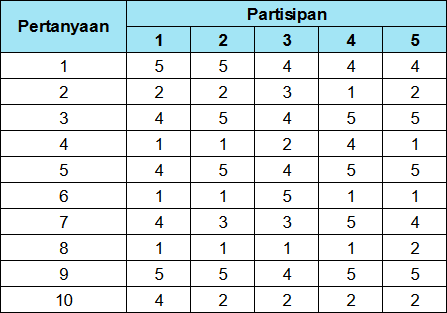
\includegraphics[width=0.7\textwidth]{hifi/chart-sus.png}
\end{figure}


\section{Konversi Penghitungan Skor SUS dan SEQ}
Berikut adalah hasil konversi perhitungan skor SUS dan skor SEQ. Daftar \textit{task} mengacu pada Lampiran \ref{chpt:skenario_hifi1}.

\begin{figure}[h]
  \centering
  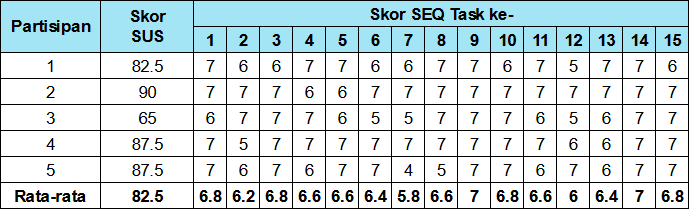
\includegraphics[width=\textwidth]{hifi/chart-sus-seq.png}
\end{figure}

% \section{Waktu Penyelesaian Task}
% \normalsize

% Berikut adalah rangkuman waktu yang diperlukan setiap partisipan untuk menyelesaikan \textit{task} yang diberikan. Daftar \textit{task} mengacu pada Lampiran \ref{chpt:skenario_hifi1}.

% \begin{figure}[h]
%   \centering
%   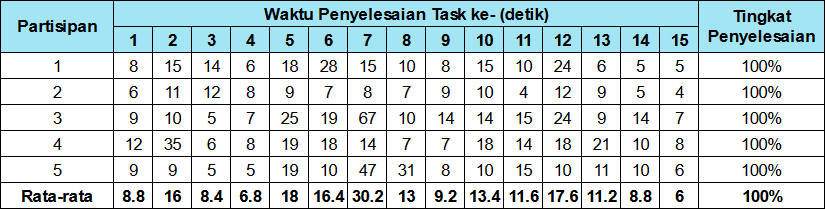
\includegraphics[width=\textwidth]{hifi/chart-penyelesaian.png}
% \end{figure}

\newpage

\section{Konversi Perhitungan Skor IMI}
Berikut adalah rata-rata nilai 3 sub skala \textit{Intrinsic Motivation Inventory}. Daftar pertanyaan pada setiap sub skala IMI mengacu pada Lampiran \ref{subsec:imi}.

\begin{figure}[h]
  \centering
  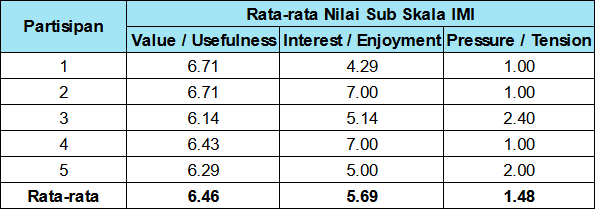
\includegraphics[width=0.95\textwidth]{hifi/chart-imi.png}
\end{figure}

\end{document}
